
% Cal Poly Thesis
% 
% based on UC Thesis format
%
% modified by Mark Barry 2/07.
%




\documentclass[12pt]{ucthesis}

\newif\ifpdf
\ifx\pdfoutput\undefined
    \pdffalse % we are not running PDFLaTeX
\else
\pdfoutput=1 % we are running PDFLaTeX
\pdftrue \fi

\usepackage{url}
\ifpdf

    \usepackage[pdftex]{graphicx}
    % Update title and author below...
    \usepackage[pdftex,plainpages=false,breaklinks=true,colorlinks=true,urlcolor=blue,citecolor=blue,%
                                       linkcolor=blue,bookmarks=true,bookmarksopen=true,%
                                       bookmarksopenlevel=3,pdfstartview=FitV,
                                       pdfauthor={!!Author goes here!!},
                                       pdftitle={!!Title goes here!!},
                                       pdfkeywords={thesis, masters, cal poly}
                                       ]{hyperref}
    %Options with pdfstartview are FitV, FitB and FitH
    \pdfcompresslevel=1

\else
    \usepackage{graphicx}
\fi

\usepackage{amssymb}
\usepackage{amsmath}
\usepackage[letterpaper]{geometry}
\usepackage[overload]{textcase}
\usepackage{color}

\definecolor{cppCommentGreen}{rgb}{0, 0.4, 0}

\usepackage{listings}
\lstset{
                language=C++,
                basicstyle=\scriptsize\ttfamily,
                keywordstyle=\color{blue}\ttfamily,
                stringstyle=\color{red}\ttfamily,
                commentstyle=\color{cppCommentGreen}\ttfamily,
                morecomment=[l][\color{magenta}]{\#}
                frame=single
                keepspaces=true
                tabsize=4
                numbers=left
                numberstyle=\scriptsize
                numbersep=5pt
}

\bibliographystyle{abbrv}

\setlength{\parindent}{0.25in} \setlength{\parskip}{6pt}

\geometry{verbose,nohead,tmargin=1.25in,bmargin=1in,lmargin=1.5in,rmargin=1.3in}

\setcounter{tocdepth}{2}


% Different font in captions (single-spaced, bold) ------------
\newcommand{\captionfonts}{\small\bf\ssp}

\makeatletter  % Allow the use of @ in command names
\long\def\@makecaption#1#2{%
  \vskip\abovecaptionskip
  \sbox\@tempboxa{{\captionfonts #1: #2}}%
  \ifdim \wd\@tempboxa >\hsize
    {\captionfonts #1: #2\par}
  \else
    \hbox to\hsize{\hfil\box\@tempboxa\hfil}%
  \fi
  \vskip\belowcaptionskip}
\makeatother   % Cancel the effect of \makeatletter
% ---------------------------------------




\begin{document}

% Declarations for Front Matter

% Update fields below!
\title{Real Time Visibility Culling With Hardware Occlusion Queries and Uniform Grids}
\author{Ilya Seletsky}
\degreemonth{June} \degreeyear{2013} \degree{Master of Science}
\defensemonth{June} \defenseyear{2013}
\numberofmembers{3} \chair{Zo\"{e} Wood, Ph.D.} \othermemberA{Foaad Khosmood, Ph.D.} \othermemberB{Aaron Keen, Ph.D.} \field{Computer Science} \campus{San Luis Obispo}
\copyrightyears{seven}	%What does this mean?

\maketitle

\begin{frontmatter}

% Custom made for Cal Poly (by Mark Barry, modified by Andrew Tsui).
\copyrightpage

% Custom made for Cal Poly (by Andrew Tsui).
\committeemembershippage

\begin{abstract}

Culling out non-visible portions of 3D scenes is important for rendering large complex worlds at an interactive frame rate.
Past 3D engines used static prebaked visibility data which was generated using complex algorithms.
Hardware Occlusion Queries are a modern feature that allows engines to determine if objects are invisible on the fly.
This allows for fully dynamic destructible and editable environments as opposed to static prebaked environments of the past.
This paper presents an algorithm that uses Hardware Occlusion Queries to cull fully dynamic scenes in real time.
This algorithm is relatively simple in comparison to other real time occlusion culling techniques, making it possible for the average developer to render large detailed scenes.
It also requires very little work from the artists who design the scenes since no portals, occluders, or other special objects need to be used.

\end{abstract}

%\begin{acknowledgements}

%   Thank you...

%\end{acknowledgements}


\tableofcontents


\listoftables

\listoffigures

\end{frontmatter}

\pagestyle{plain}




\renewcommand{\baselinestretch}{1.66}


% ------------- Main chapters here --------------------





\chapter{Introduction}
\label{intro}

\section{Real Time Graphics}
\label{real-time-graphics}

Real time computer graphics are needed for CAD applications, simulations, video games, and even for just displaying the user interface of an operating system.
Computer graphics can be non-real time, for example when doing CGI for a movie.
Each frame can take hours to render, and the result is a very photorealistic image that looks like it is part of the movie itself.
Millions of frames are generated only for each still frame to be visible for a fraction of a second until the next frame to give the illusion of motion.
Real time graphics also display a frame for only a fraction of a second but are rendered on the fly right as the user is controlling the application.
This means the computer only has 33.33 milliseconds if trying to render at 30 frames per second (FPS).
Most computer monitors update at 60 Hz so real time graphics typically strive for 60 FPS giving an even smoother experience, and this means the computer now only has 16.66 milliseconds to render a frame.
Maintining a smooth, also known as interactive, framerate is important for ensuring the user has a good experience controlling the application.\cite{Interactive}

Real time graphics are a challenge because a scene may need to be rendered with the quality that looks as close to non-real time graphics as possible like the scene from Battlefield 3 in figure \ref{fig:bf3}.
Many calculations need to be performed to produce the resulting geometry and lighting for a frame.
Photorealistic real time graphics get away with many shortcuts to look as real as possible.
The result may not be completely realistic and does not simulate the physics of light as accurately as non-real time graphics, but the resulting image still looks good.
It is possible to have non-photo realistic graphics as well like the character from Borderlands 2 in figure \ref{fig:borderlands2}, but those too require a large amount of processing power.

\begin{figure}
\begin{center}

\includegraphics[width=\textwidth]{Images/BF3.jpg}
\captionfonts
\caption[Battlefield 3]{The photorealistic real time graphics of Battlefield 3. (TODO: make these images side by side and figure out how to cite them)}
\label{fig:bf3}

\includegraphics[width=\textwidth]{Images/Borderlands_2.png}
\captionfonts
\caption[Borderlands 2]{The comic book style of Borderlands 2.}
\label{fig:borderlands2}
\end{center}
\end{figure}

\section{The Power of Graphics Processing Units}
\label{gpu}
Computers have dedicated Graphics Processing Units(GPU) to help with rendering these images.
Modern GPUs are built to perform a single operation on large amounts of data in parallel, which makes them useful for non-graphics applications as well with the help of tools like CUDA.\cite{FermiArch}
The graphics pipeline of current GPUs is built to work with triangles.\cite{d3d11-pipeline}
Geometry is represented by a series of vertices making up the triangles.
The GPU then puts the geometry through various stages where all of the vertices are transformed from 3D world space to 2D screen space, and are then rasterized to the screen.
There are large amounts of vertices and large amounts of pixels to be rasterized.
The GPU runs a single algorithm at a time on these large amounts of data in parallel.
This is why modern hardware can render many triangles with relative ease.
For example, the dPVS paper has one scene displaying approximately 180,000 triangles at about 68 FPS.\cite{dpvs}

\section{Visibility Culling}
\label{visibility-culling}

Modern graphics hardware is becoming better and better at rendering large detailed environments in real time.
Games like Rage by idSoftware, Battlefield 3 by Dice, Crysis by Crytek, and Just Cause 2 by Avalanche Studios, have maps on an large scale with drawing distances of several kilometers.
These kinds of environments are achievable by avoiding drawing as much of the world as possible.\cite{heir-occ-map, large-occluders, Vis-Computations-Densely-Occluded, Portal-culling, Cryengine-culling-explained, Portals-mirrors, dpvs, cryengine3, culling-bf, CHC, CHCpp}
This is the job of a visibility culling algorithm.
The scene is viewed through a virtual camera.
Objects visible to the camera fit within the frustum as shown in figure \ref{fig:frustum}.
It is relatively easy to avoid drawing portions of the scene that are not in the camera's field of view with view frustum culling by checking if the object is inside this frustum.
(TODO: cite: http://www.lighthouse3d.com/tutorials/view-frustum-culling/)
If a camera is looking at a wall or a mountain in the distance, it is also best to avoid drawing the objects behind them.
Figuring out that objects are behind other objects in real time is a challenge but can save many unnecessary draw calls to the GPU.

\begin{figure}
\begin{center}
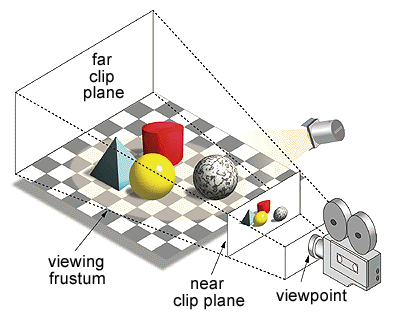
\includegraphics[width=0.5\textwidth]{Images/frustum.png}
\captionfonts
\caption[View Frustum]{A camera and its view frustum. A frustum is a pyramid with its top cut off. Objects within the frustum are visible.(TODO cite:http://www.pcmag.com/encyclopedia/term/61771/viewing-frustum)}
\label{fig:frustum}
\end{center}
\end{figure}

A visibility culling algorithm should do its best to determine which objects are not visible to the camera.
The algorithm may generate some false positives and determine that a few objects are visible when they really are not.
Since the GPU is able to render geometry very quickly, a few extra objects will just cause a negligible performance drop.\cite{large-occluders}
The visual quality starts to suffer if objects go missing that should actually be there, so false negatives on visibility should be avoided.
Most of the visibility culling work happens on the CPU while the GPU does all the rendering.
If the CPU is doing too much work finding which objects the GPU should not render, the performance may be worse than if there is no occlusion culling algorithm in the first place.
A good algorithm must strike the perfect balance where the CPU is not working too hard but is still saving the GPU a lot of work, giving a considerable performance increase.

\section{Dynamic Environments}
\label{dynamic-environments}

Static environments of the past used prebaking steps to compute expensive operations such as lighting and visibility.
Nowadays more is possible with fully destructible environments and WYSIWYG level editors built right into the game.
Environments can be made out of modular set pieces and put together like lego blocks.
Figures \ref{fig:hangar-view} and \ref{fig:hangar-peices} show an example.
A wall, column, railing, ladder, or tree may be reused many times in the level, saving artists a lot of work as well as keeping memory down due to loading in one resource and reusing it many times.

\begin{figure}
\begin{center}
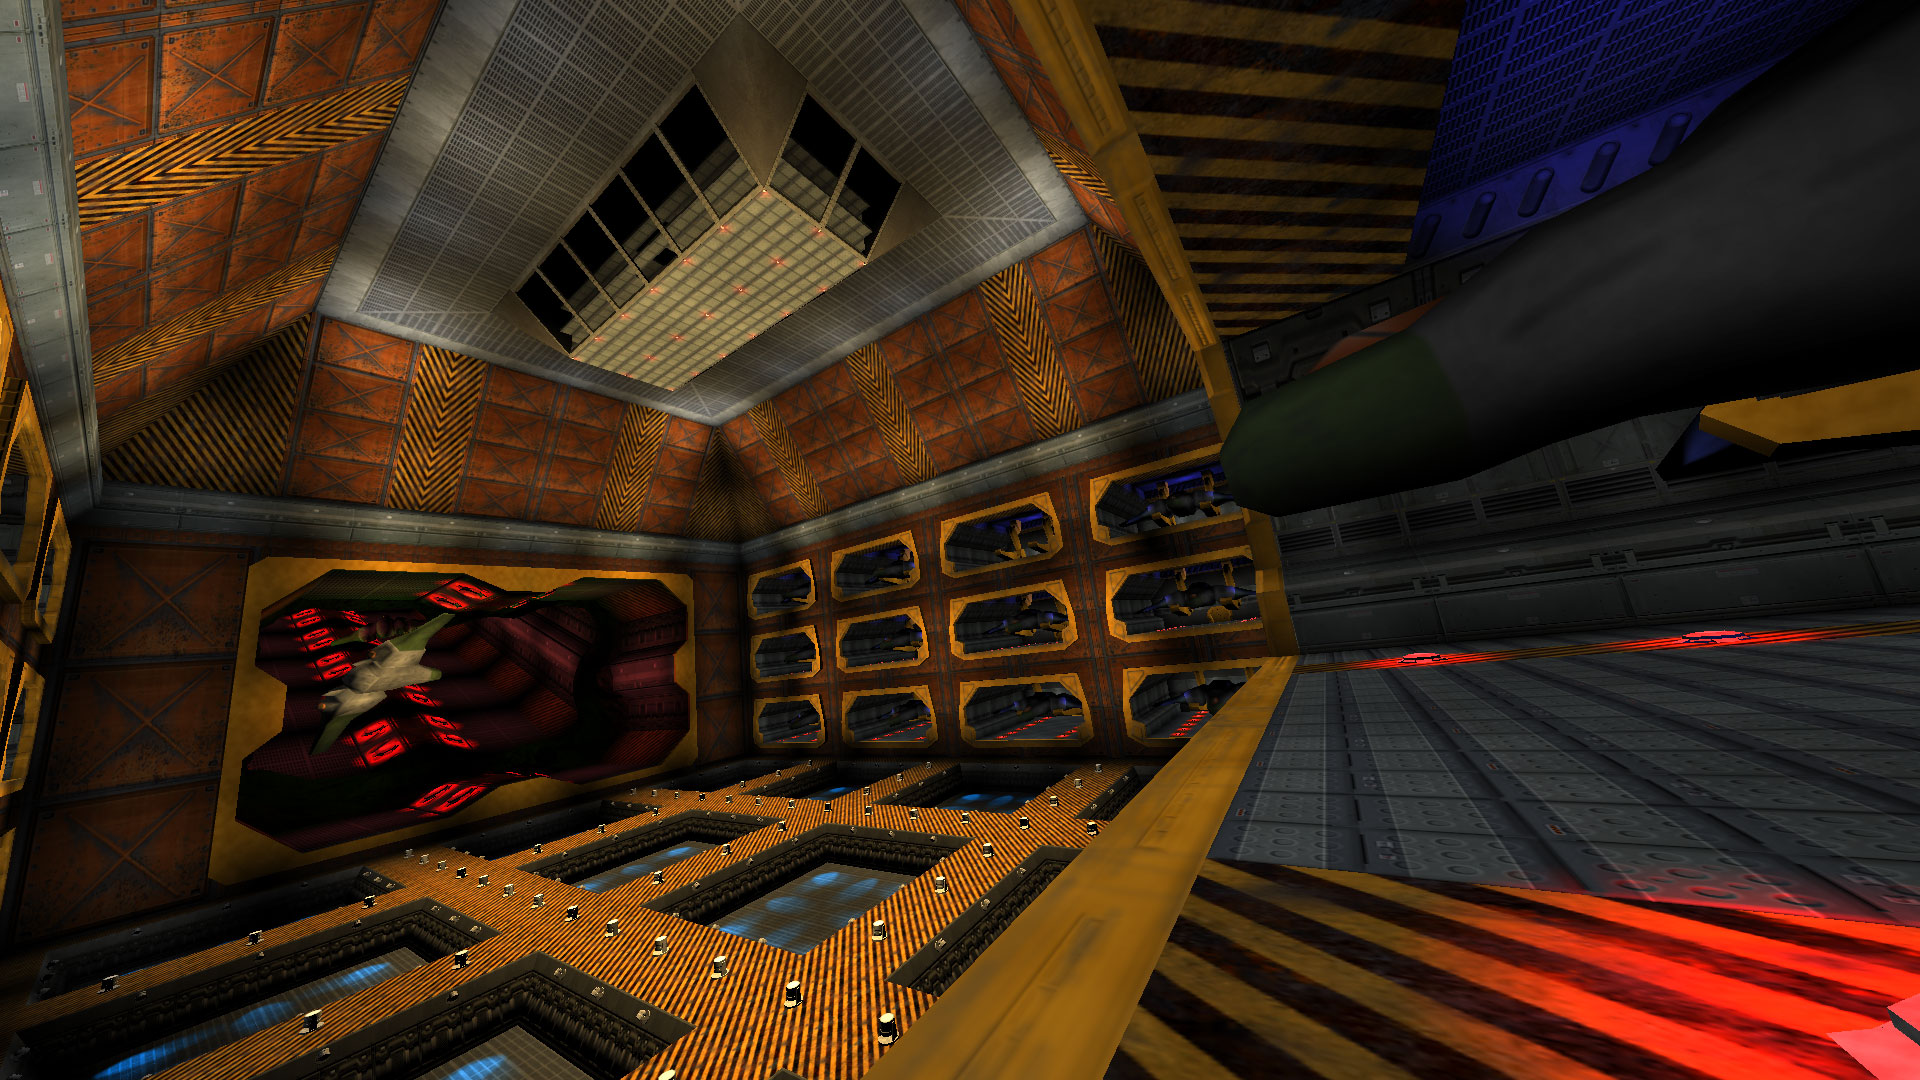
\includegraphics[width=\textwidth]{Images/Hangar.jpg}
\captionfonts
\caption[Hangar]{A view of the Hangar in the environment made for this project.}
\label{fig:hangar-view}
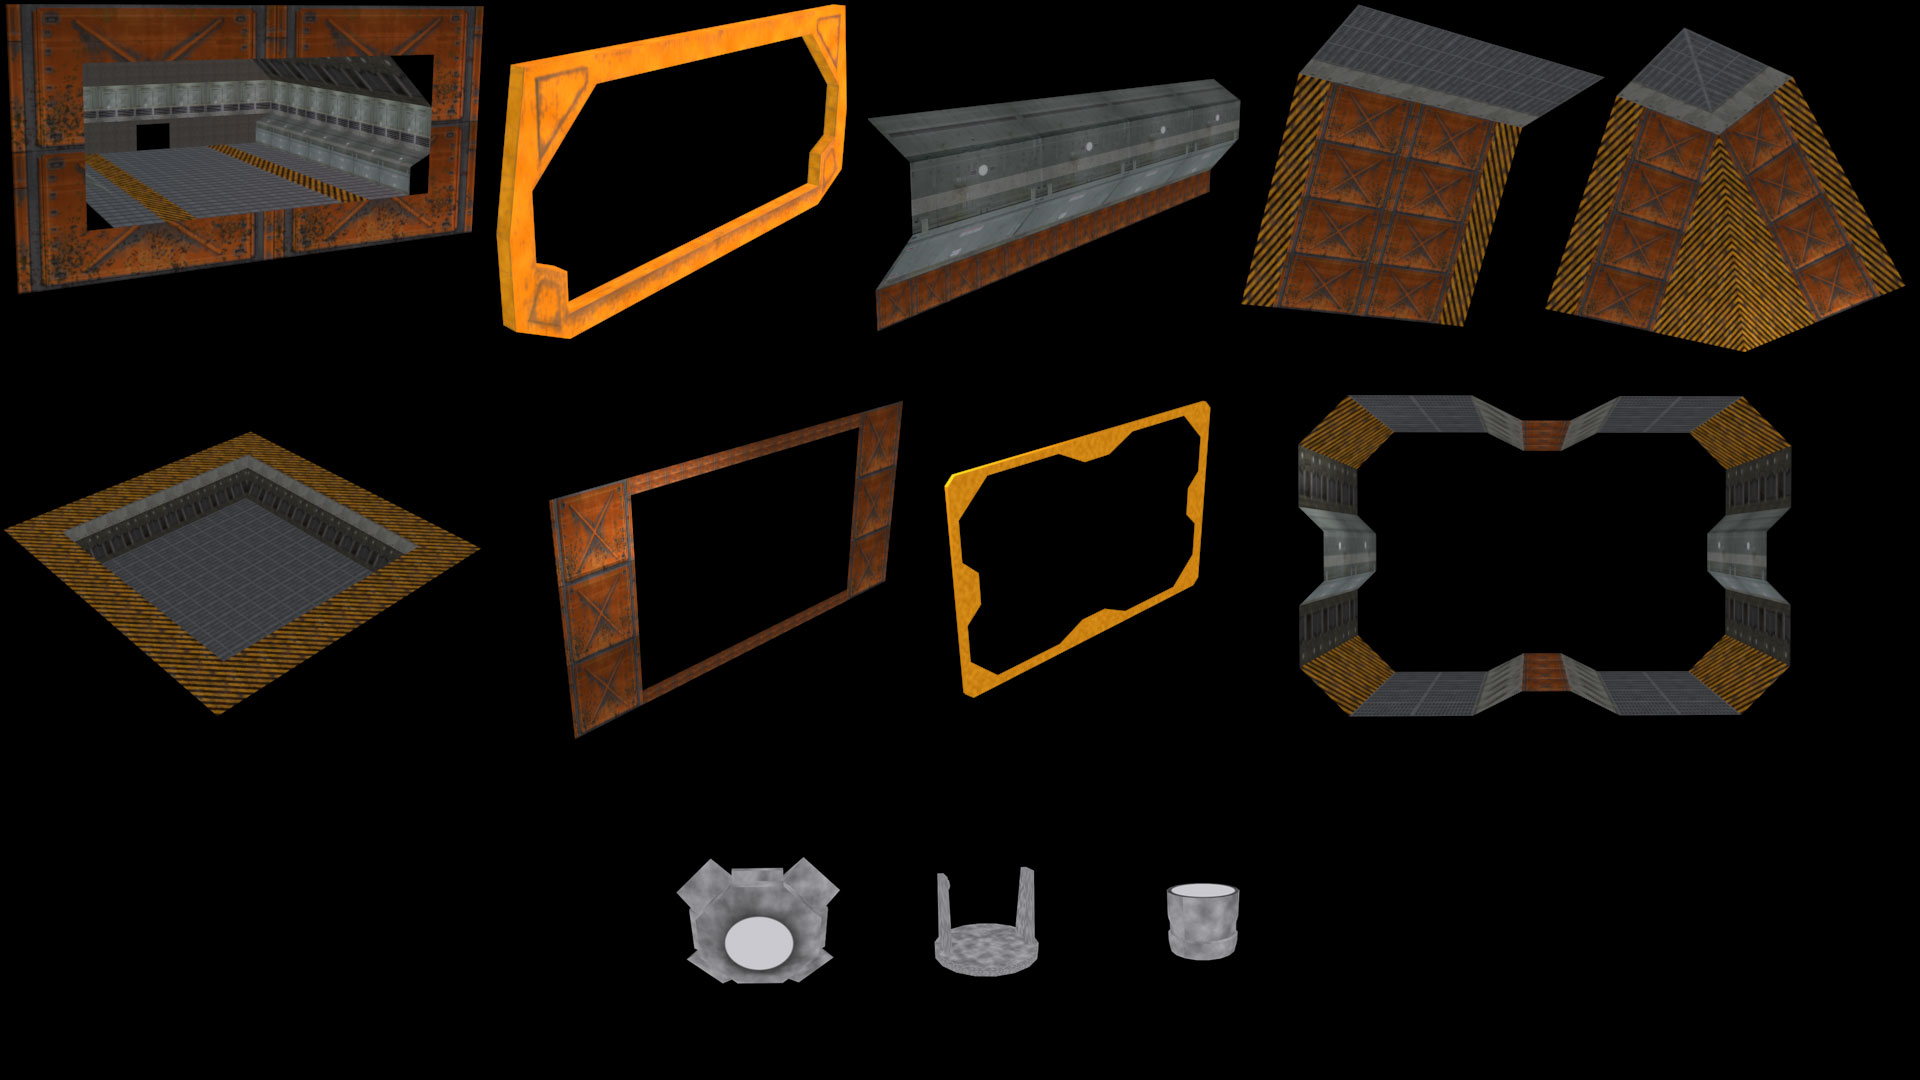
\includegraphics[width=\textwidth]{Images/Peices.jpg}
\captionfonts
\caption[Hangar Modular Pieces]{Some of the modular pieces that make up the hangar.}
\label{fig:hangar-peices}
\end{center}
\end{figure}

While designing levels, the artists would work with these objects by throwing in new ones, moving them around, and deleting them.
The level editor's performance can be greatly increased if it uses a real time visibility culling  algorithm.
In a game with destructible environments, these same objects can now be moved around and destroyed on the fly.
With all of this happening, visibility data needs to update automatically and in real time.
In fact, the level editor can be either built right into the game or just use the same 3D engine that that game uses.
This lets artists see exactly how the environment looks as if they were currently playing the game.

\section{Artist Placed Hint Objects}
\label{artist-placed-hint-objects}

Sometimes an algorithm can not figure out the best way to perform visibility culling in every situation so artists need to place hint objects.
Hint objects allow an engine to avoid making calculations since the information is given by the designer.
This creates a lot of extra work for the artists and can be really tedious.
Artists now need to be educated on the technical inner workings of the engine so they can place the hint objects in the best way.
Even then, artists may still not do it the best way.

Portals are objects that are placed in windows and doorways linking different rooms or zones of an indoor environment.\cite{Vis-Computations-Densely-Occluded, Doom3-source-review, Portal-culling}
They help the engine render objects only visible to the camera through the portal geometry and not through the walls.
They are effective in static environments where the artists know a door or window will always be around.
However if someone takes a rocket launcher and blows up a hole in a wall, there is no artist placed portal there to help the engine.
The engine will not necessarily be smart enough to know how to best place a portal there since any kind of arbitrary destruction can take place.
The zones divided by portals are often static as well and the engine would need to somehow figure out how to create new zones on the fly.
Portals can also be very tedious for the level designers to keep track of as they are constantly iterating on the design of a level.

Occluder geometry is also often used in modern game engines.
Modelers can make a low detail version of a mesh as shown in figure \ref{fig:occluder-geometry}.\cite{culling-bf}
The engine can then do ray intersection tests against all triangles in this mesh to test if some object is behind the geometry.\cite{Cryengine-culling-explained}
Engines that do software occlusion culling render these meshes CPU side rather than rendering the detailed geometry the GPU powered hardware occlusion queries would render.
Making these low resolution meshes that are used specifically for occlusion culling creates extra work for modelers.
If an object is destructible, the low resolution mesh must somehow be deformable along with the high resolution mesh it represents.

\begin{figure}
\begin{center}
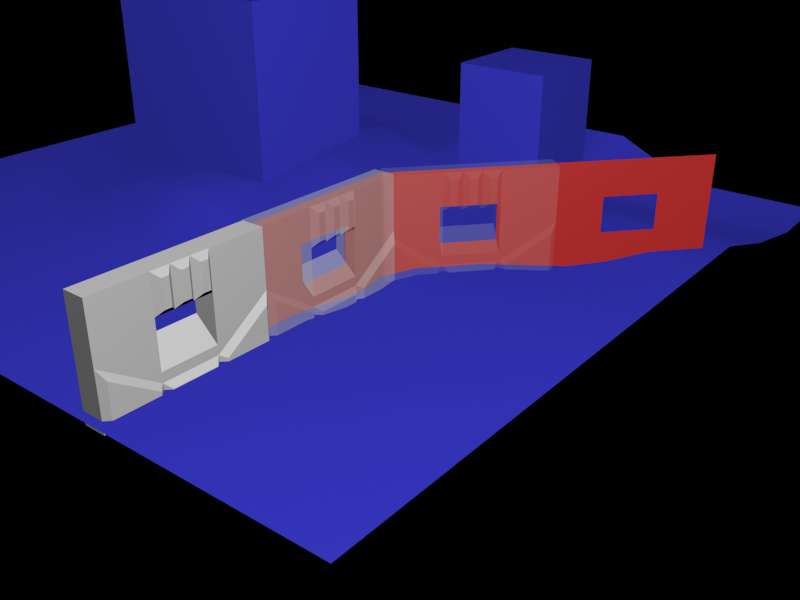
\includegraphics[width=0.75\textwidth]{Images/OccluderGeomFig.jpg}
\captionfonts
\caption[Occluder Geometry]{The detailed wall and its associated low detail occluder geometry shown in red.}
\label{fig:occluder-geometry}
\end{center}
\end{figure}

\section{Our Contribution}
\label{our-contribution}
This paper presents a simple high performing visibility culling algorithm that any 3D engine can integrate.
It allows rendering of large outdoor worlds that are seamlessly combined with detailed indoor architecture.
It requires hardware that supports occlusion queries which allow the GPU to report how many pixels of an object are not occluded by other objects.\cite{GpuGem-Queries}

This algorithm avoids the added complexity of a software rasterizer.
Similar algorithms use software occlusion queries in order to avoid the delay when retrieving hardware occlusion query results.\cite{culling-bf}
This would require software rasterizers to be written that run on the CPU instead of making use of the hardware that performs this task far more efficiently.
The paper also presents a method for combining the use of queries with effective render state sorting.

There is very minimal artist intervention required when designing environments using this algorithm.
The high detail objects that are rendered are also automatically occluding parts of the environment without the need for artists to manually tweak things with portals or special occluding geometry.

A front to back view frustum scene traversal algorithm is presented in order to make the query results optimal.
If the objects in front are drawn before the objects behind, the objects behind can be tested against those already drawn objects.
This reduces false positives in visibility tests because objects in back aren't mistakenly determined to be visible if the objects in front are processed first.

\chapter{Background}
\label{background}

This section provides an overview of computer graphics concepts relevant to this paper.
First, we describe how software interfaces with the GPU in Section \ref{3d-graphics-api}.
Sections \ref{z-buffer-and-depth-test} and \ref{other-tests} describe tests that are part of the graphics pipeline for preventing pixels from being written to the screen.
Next, the application of the pipeline's tests for use in Hardware Occlusion Queries is explained in section \ref{hardware-occlusion-queries}.
Section \ref{spatial-data-structures} is an overview of spatial data structures that are essential in most graphics algorithms.

\section{3D Graphics API}
\label{3d-graphics-api}

There are many Application Programming Interfaces (APIs) for allowing software to interface with the graphics pipeline.
The pipeline may be running in software on the CPU or hardware accelerated by the GPU.
The APIs allow software to change states in the graphics pipeline and to issue draw calls.
Two widely used APIs on personal computers are OpenGL and Direct 3D.\cite{about-openGL, about-direct3D}
The APIs may be different but the computer graphics concepts remain the same.
The project in this paper was built with OpenGL but is portable to Direct3D.

\subsection{OpenGL}
\label{openGl}

OpenGL is a cross platform standard for rendering 3D graphics maintained by the Khronos group.\cite{about-openGL}
OpenGL APIs are available on many systems such as Windows, Linux, and MacOS.
OpenGL ES is the mobile version bringing 3D graphics to iPhone and Android devices.\cite{ios-glEs, android-glEs}

\subsection{Direct3D}
\label{direct3d}

Direct3D is part of Microsoft's DirectX package.\cite{about-direct3D}
It is available on platforms such as Windows, Xbox, and Windows 8 phones.
At the time of this writing, DirectX 11 is the latest version and has some features that make it easier for multithreaded applications to issue draw calls in parallel.\cite{d3d11-parallel}

\section{Z Buffer and Depth Test}
\label{z-buffer-and-depth-test}

The z buffer is allocated along with the Frame Buffer where the image is rendered.
A depth value gets computed for each fragment, which corresponds to a pixel of a triangle as it gets rasterized by the graphics hardware.
The early z test happens right before the work of the fragment shader where the color of the pixel gets computed and written.\cite{d3d11-pipeline}
The graphics hardware compares the depth value of the fragment about to be written with the value already written.
By default, OpenGL is set to allow a fragment to pass if the new value is less than the current value.\cite{gl-depth-func}
This test is used for solid geometry only, which usually makes up most of the geometry in the scene.
This means solid polygons do not need to be presorted by depth to have the scene look correct.
The depth test is also essential for hardware occlusion queries which will be described later.

\begin{figure}
\begin{center}
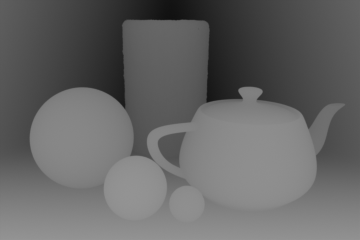
\includegraphics[width=0.5\textwidth]{Images/Z_buffer.png}
\captionfonts
\caption[Z Buffer]{Example of a Z Buffer}
\label{fig:z-buffer}
\end{center}
\end{figure}

\section{Other Tests}
\label{other-tests}

There are a few other tests done by the graphics pipeline that can eliminate a fragment.\cite{GpuGem-Occlusion}
The scissor test allows rectangle on the render target to be set.
Anything outside the scissor rectangle is not rasterized.
The stencil test uses a buffer similar to the z buffer.\cite{d3d11-pipeline}
Values can be rasterized to the stencil buffer and tested in some way.
The alpha test prevents a fragment from being rendered if the alpha, also known as opacity, portion of the color is below a certain threshold.
These tests, along with the previously mentioned depth test, can be enabled or disabled depending on what is needed for a draw call.

\section{Hardware Occlusion Queries}
\label{hardware-occlusion-queries}

The hardware occlusion query is a relatively new feature that is essential to this paper.
The query measures how many fragments have passed for a set of draw calls.
The fragments must pass all tests of the graphics pipeline described in Sections \ref{z-buffer-and-depth-test} and \ref{other-tests} to contribute to the query results.

A possible use of a hardware occlusion query is to first render an object's bounding box.
The box is composed of only 12 triangles so it has very little impact on performance.
The box should be rendered during a query with color and depth writing disabled.
This means the box will never affect the final image, but it will still go through the full pipeline.
The depth test should be enabled so fragments of the box can be rejected if other objects already rendered are occluding the box.
Objects in the scene should be rendered front to back so occludees in back are tested against the occluders in front.

After testing with the invisible bounding box, retreive the results of the query.
If any fragments of the box passed, the real object is probably visible.
Now color writing and depth writing should be enabled as the real object is rendered.
With depth writing enabled, the object is written to the z buffer and can now serve as an occluder for more objects that are behind it.

\subsection{CPU Stalls}
\label{cpu-stalls}

The approach just described negatively affects performance.
The problem with hardware occlusion queries is their results may not be ready to read back when expected.\cite{GpuGem-Occlusion, GpuGem-Queries, CHC, CHCpp}
The GPU has its own memory and processor.
Data must travel across a bus on the motherboard between the CPU and GPU.
Draw calls issued by the CPU are non-blocking and are stored in a buffer for the GPU to execute whenever it gets around to it.
However, retreiving a value back from the GPU can cause a stall since the applicaiton must wait a few milliseconds for the data to travel across the bus.
The query result may be available about 3 to 4 frames later.
When there are thousands of objects to draw, the stalls add up.
The challenge with using hardware occlusion queries is finding a way to effectively use them in later frames to reduce CPU stalls but still save the GPU from drawing too many unnecessary objects.

\subsection{Conditonal Rendering}
\label{conditional-rendering}

Conditional rendering allows the results of a query to be used in the same frame.
The GPU knows the results of a query after a draw call since the data is local and does not need to travel across the bus.
The CPU still issues all potentially unnecessary draw calls but the GPU ignores them if the draw call depends on the results of a query.
If hardware support for conditional rendering is not available, it is forced to run in software and and causes a drop in performance.
This does not prevent unnecessary traversals of portions of the scene by the CPU that may be invisible.
It is simply a way to tell the GPU to ignore an already issed draw call.

\section{Spatial Data Structures}
\label{spatial-data-structures}

Spatial data structures accelerate spatial queries by reducing the search space.
View Frustum Culling described earlier is an example of a spatial query that finds objects in the scene that are within the bounds of the frustum.
Another example is to find all objects within a radius or axis aligned bounding box.
Many spatial data structures exist, each with their own pros and cons.
The right structure should be chosen depending on the application.
Chapter \ref{related-work} provides an overview of other visibility culling techniques and what spatial data structures were chosen.

The uniform grid is one of the simplest structures.
It provides a uniform subdivision of space.
Objects have a bounding box, and are binned into cells of the grid that overlap with the bounding box.\cite{culling-bf, applications-spatial, chess}
Querying for objects in the grid simply requires indexing into cells of the grid which intersect with the spatial query.
This is an optimal structure for cases when objects are evenly distributed in the world.
This could be an issue if the scene has hundreds of objects in one cell while the rest of the cells have very sparse amounts of objects.
Querying within the bounds of that cell would not reduce the search space by very much.

A spatial hash is similar to a grid but allows the scene to not be constrained within predefined bounds.
The hash has buckets just like a grid has cells, but multiple cells can hash to one bucket.
For example, if the grid is allocated to hold 5 by 5 cells, grid cell (1, 3) would hash to the same bucket as (6, 3).
A standard grid would not be able to handle cell (6, 3) since that is outside of the grid.

The quad tree is a heirarchical datastructure that handles unevenly distributed objects better.\cite{applications-spatial}
It distributes the objects by progressively dividing each cell into four smaller cells until each cell has a small enough number of objects for the application.
Since it is structured as a tree, many cells get filtered out along the traversal before reaching the leaf cells.
Once a path down a traversal is not taken, all child nodes in the heirarchy are automatically ignored.
This helps filter out many more potential objects than a grid earlier on in the search.
Octrees are a 3D extension of quadtrees and divide each cell into 8 children rather than 4.
This can be extended to other dimensions beyond that as well, to help with problems mapped to multiple dimensions.\cite{applications-spatial}

Bounding volume heirarchies are another common heirarchical structure.\cite{BVH}
This organizes the scene by having each node be a bounding box that contains the bounding boxes of all of its children.
The leaves in the tree contain the objects themselves.
As the tree is traversed, the bounding box of the query is used to determine what set of children to follow if their bounding box also intersects the query object.
A well balanced tree structure gives the best overall performance.
This kind of structure allows any arbitrary scene layout while grids and quadtrees are constrained to hold the scene within predefined bounds.

K-D trees recursively divide up a space into two halves with axis aligned planes.\cite{Vis-Computations-Densely-Occluded, Doom3-source-review}
They can look a bit similarly to Octrees in some situations.
The space is divided in a way that evenly distributes the geometry between the two planes, handling the poorer distribution of Octrees and Uniform Grids.
Binary Space Partitioning trees are similar except they divide space with arbitrary planes.
The final result is an even better distribution of geometry that results in a more balanced tree, but the algorithm for computing the tree is more time consuming.

\chapter{Related Work}
\label{related-work}

Visibility Culling has been performed with a variety of methods over the last decades.
Many clever tricks have been found that take advantage of certain assumptions about a scene, sometimes limiting what kinds of scenes are possible.
Keeping a scene static while performing a walkthrough of an indoor area is common.\cite{Vis-Computations-Densely-Occluded, Portals-mirrors, Doom3-source-review}
Some software-based occlusion culling solutions have been used as well in order to avoid the CPU stalls of hardware occlusion queries.\cite{spliter, culling-bf}

One visibility culling algorithm uses mathematical properties of convex polyhedral objects to determine visibility on the fly.\cite{large-occluders}
Coorg and Teller find objects in the scene that serve as large occluders, and avoid testing against smaller objects that would not serve as effective occluders.
Since the environments are made of collections of convex geometry, it is possible to compute separating and supporting planes from pairs of objects and compute whether or not one object is occluding another.
The algorithm was developed at a time when the z buffer may be unavailable or done slowly in software, so this algorithm was able to avoid relying on the z buffer.

Portal culling, which was mentioned earlier, is effective for indoor environments but not as effective in outdoor environments.\cite{Portals-mirrors}
If the environment is subdivided into zones, only geometry in zones that are determined to be visible gets rendered.
The camera's initial view frustum gets computed.
The geometry in the zone the camera is located is then rendered.
If the geometry of a portal is visible to the camera, a new smaller view frustum spawns off that simulates the view through the portal into the adjacent zone.
The scene's zones are traversed this way until no more portals are determined to be visible.

\begin{figure}
\begin{center}
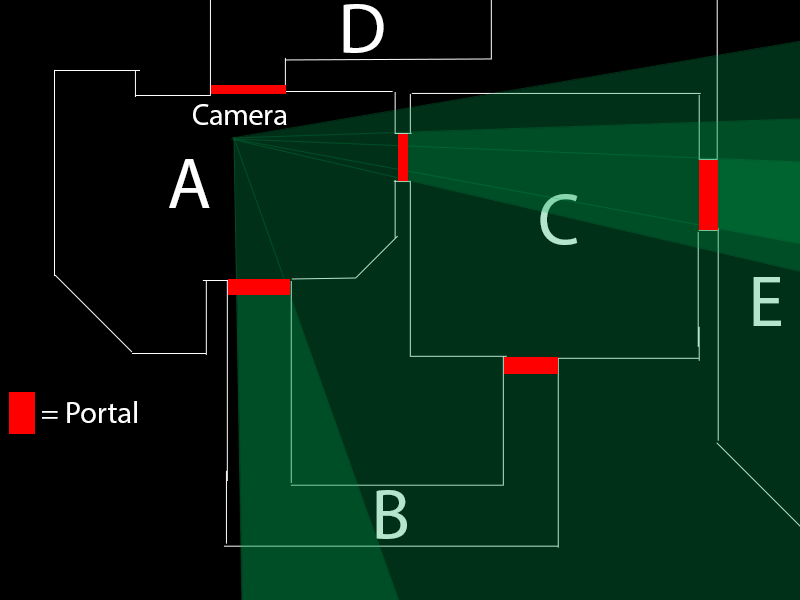
\includegraphics[width=0.75\textwidth]{Images/Portal-Culling.png}
\captionfonts
\caption[Portal Culling]{An example of portal culling at work.  Zones A, B, C, and E are rendered.}
\label{fig:portal-culling}
\end{center}
\end{figure}

Teller finds another way to compute visibility in environments made of convex polyhedral geometry.\cite{Vis-Computations-Densely-Occluded}
This time the scene is preprocessed ahead of time with his algorithm.
The algorithm is applied in id Software's idTech 4 engine used in games like Doom 3 and Quake 4.\cite{Doom3-source-review}
Areas of the environment are subdivided and stored in a BSP tree.
Portals need to be placed by the level designers in crucial areas like doorways and windows to allow the algorithm to compute zones.
The algorithm finds mini areas and they are joined into zones with a flood filling algorithm.
Solid geometry and artist placed portals determine the bounds of zones.
Without artist placed portals, Doom 3 renders the entire level rather than only visible rooms.
In 1992, this algorithm was said to take hours of CPU time, but was able to store the processed scene in a fraction of the space.
Id software's previous titles, Quake 1 through 3, used to run a similar algorithm offline in a separate utility.
Artists made levels in a separate tool and converted the levels to a format loadable by the game.
Doom 3 can now run this algorithm right before loading a level and the process is built right into the game.
This way the game can ship with the levels in their editable form for people to look at with the built in map editor.

Zang, Manocha, Hudson, and Hoff have developed an algorithm that uses a heirarchy of occlusion maps.\cite{heir-occ-map}
Occlusion maps are similar to the z buffer.
In this algorithm a heirarchy of buffers is created, which are similar to the z buffer at different levels of detail.
Occluders are rendered to this buffer.
Occludees then are tested against the right buffer depending on how big they are on the screen by testing and rasterizing a bounding rectangle.
An algorithm similar to this was applied in Ubisoft's Splinter Cell Conviction.\cite{spliter}
They were able to acheive about 20,000 queries every frame on the Xbox 360.

The Frostbite 2 Engine developed by Dice is a great example of modern occlusion culling.\cite{culling-bf}
This engine effectively supports destructible environments in both indoor and outdoor settings as shown in the game Battlefield 3.
It shows off the capabilities of modern high end hardware as well as managing to run on dated hardware with a lower spec profile.
Typically hierarchical data structures such as Octrees, Bounding Volume Hierarchies, or BSP Trees are used for 3D scene management.\cite{CHC, CHCpp, GpuGem-Queries, dpvs}
However, the developers of Battlefield 3 found they were able to push more performance with a uniform grid.
Modern parallel computing architectures handle the linear arrays of a grid much better than the branch heavy traversal of the hierarchical structures.\cite{culling-bf}
The lack of branching creates predictable data access that is cache coherent and allows variaous parallel algorithms to operate more efficiently.
The visibility culling algorithm relies on artist generated low detail large occluder geometry that is rasterized software-side to a low resolution depth buffer.
This requires a software rasterizer capable of rendering arbitrary geometry to be implemented.
Objects such as tanks or soldiers have their bounding rectangle tested against this buffer similarly to how a hardware occlusion query would operate before being queued up for the hardware to render.

\begin{figure}
\begin{center}
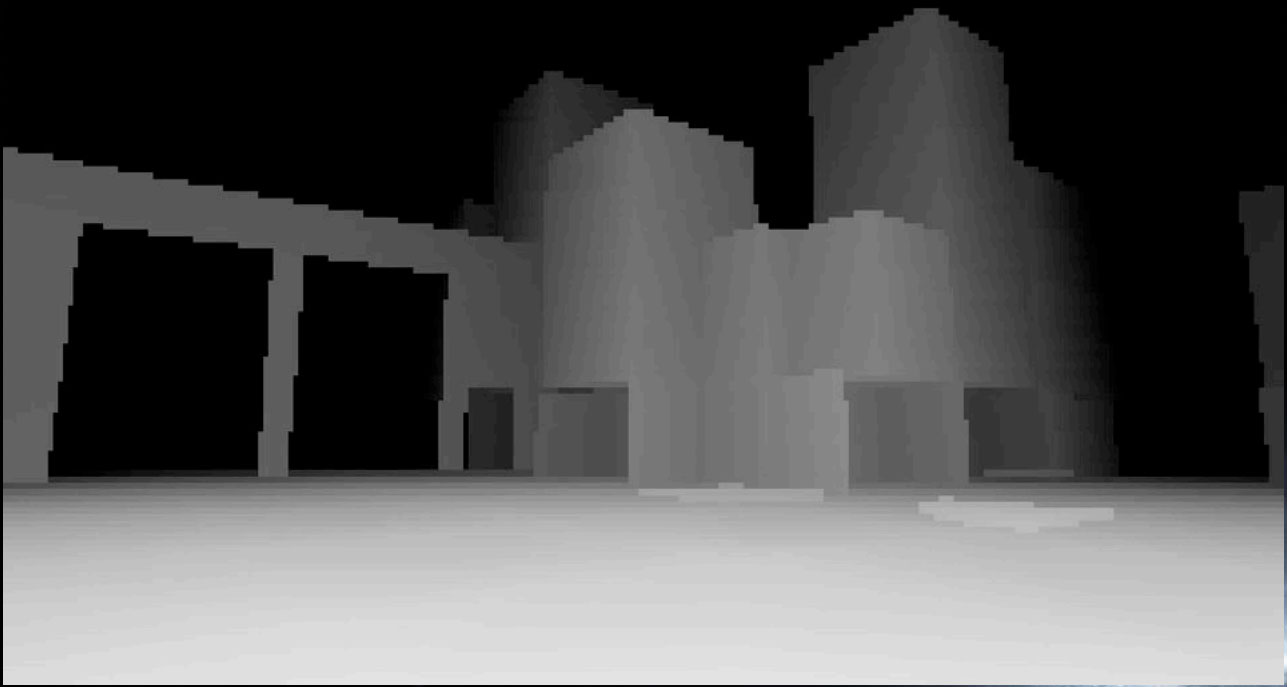
\includegraphics[width=0.75\textwidth]{Images/Bf3Buffer.jpg}
\captionfonts
\caption[Software Z Buffer Buffer]{The low resolution software z buffer from a scene in Battlefield 3. (TODO: cite Culling the battlefield pres)}
\label{fig:softare-z}
\end{center}
\end{figure}

CryENGINE 3, used for games like Crysis 2 and Farcry 3, is another modern game engine capable of rendering large indoor and outdoor environments effectively.\cite{cryengine3, Cryengine-culling-explained}
Cryengine uses what is called a coverage buffer but avoids implementing a full arbitrary geometry rasterizer by reading back the z buffer from the hardware and using it in later frames.
As the camera moves around, the coverage buffer needs to be adjusted to correspond more closely to how the current frame looks.
Cryengine reprojects the buffer with the transform of the current camera and then fills in any holes.
After this, like Frostbite 2, objects' bounding rectangles are rasterized and tested against the contents of the coverage buffer.
Cryengine also allows for use of portals and occlusion geometry that they refer to as antiportals to further augment the visibulity culling algorithm.

\begin{figure}
\begin{center}
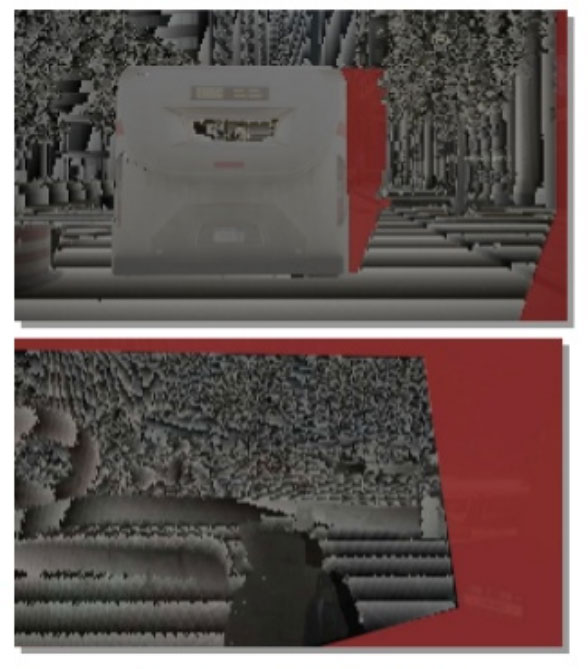
\includegraphics[width=0.5\textwidth]{Images/CryCoverage.jpg}
\captionfonts
\caption[Cry Engine Coverage Buffer]{The coverage buffer used in CryENGINE 3.  The red portions are the holes after reprojecting from previous frames to the current camera angle. (TODO: cite Secrets of Cryengine 3 Pres)}
\label{fig:cry-coverage}
\end{center}
\end{figure}

The dPVS algorithm developed by Aila and Miettenen is another similar algorithm capable of rendering large dynamic environments.\cite{dpvs}
Their system allows for a combination of various occlusion culling algorithms such as portals and queries.
The scene is organized by a K-D tree.
This data structure is normally used best in static environments, but this algorithm is able to effectively recompute the structure on the fly.
They too use a coverage buffer for occlusion queries where the sillhouettes of objects are rasterized.
Queries are then run against this coverage buffer.

The Coherent Heirarchical Culling algorithm uses the same hardware occlusion queries that this paper uses.\cite{CHC, CHCpp}
This algorithm allows a scene managed by a Bounding Volume Heirarchy to effectively use queries.
Temporal coherence is taken advantage of, meaning the results of queries from previous frames are not likely to change.
As the tree of the bounding volume heirarchy is traversed, the visibility results of nodes are used in later frames.
Since this is a heirarchy, entire portions of the scene can be culled out for a number of frames.
They make no mention on whether or not objects noticeably pop in late with this algorithm.

\chapter{Visbility Culling Algorithm}
\label{visibility-culling-algorithm}

In this chapter, we describe the steps in the visibility culling algorithm. (TODO: write this paragraph when I'm done revising the chapter)

\section{Algorithm Overview}
\label{algorithm-overview}

This algorithm stores the scene in a uniform grid.
A grid is easy to keep updated with the contents of a fully dynamic scene.
Objects that move around can use their Axis Aligned Bounding Box to determine which cells they need to be tracked in.
A grid's structure does not need to be recomputed as the scene changes in real time like the other static structures would.
There is no branching as the structure is traversed, making it easier to process the scene in one pass with occlusion queries.
The results of visibility changes in a heirarchical structure would take a few extra frames to propagate, possibly increasing the likelyhood of noticeable popping artifacts.

Figure \ref{fig:algorithm-00} shows a top view of a full scene and the field of view of a camera that is looking at the scene.
The grid cells that intersect the camera's view frustum are traversed in front to back order relative to the camera.
For each cell that gets traversed, an occlusion query is issued.
Color and depth write are disabled and just the box of the cell is rendered.

\begin{figure}
\begin{center}
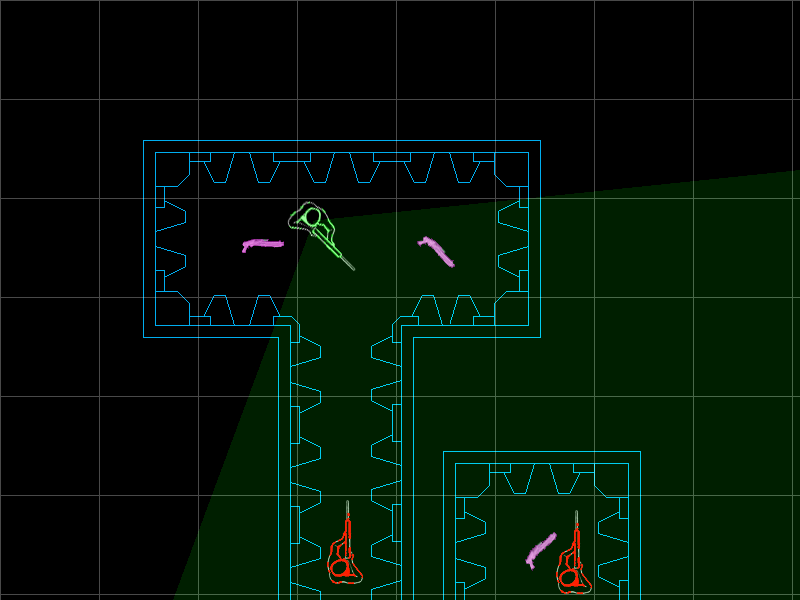
\includegraphics[width=0.75\textwidth]{Images/sceneAlgorithm/00.png}
\captionfonts
\caption[A Scene]{The overall scene partitioned by a uniform grid.  The green cone represents the camera's field of view.}
\label{fig:algorithm-00}
\end{center}
\end{figure}

If the cell is marked visible in a previous frame, the cell's objects are now rendered with depth write only but color write turned off.
This way objects are put into the z buffer to occlude cells farther back but none of the expensive lighting and shading calculations are performed.
The cell's objects are also queued up to later be rendered in full color.
Figure \ref{fig:algorithm-01} shows a moment in time during the frustum traversal and Figure \ref{fig:algorithm-02} shows a fully traversed scene.

\begin{figure}
\begin{center}
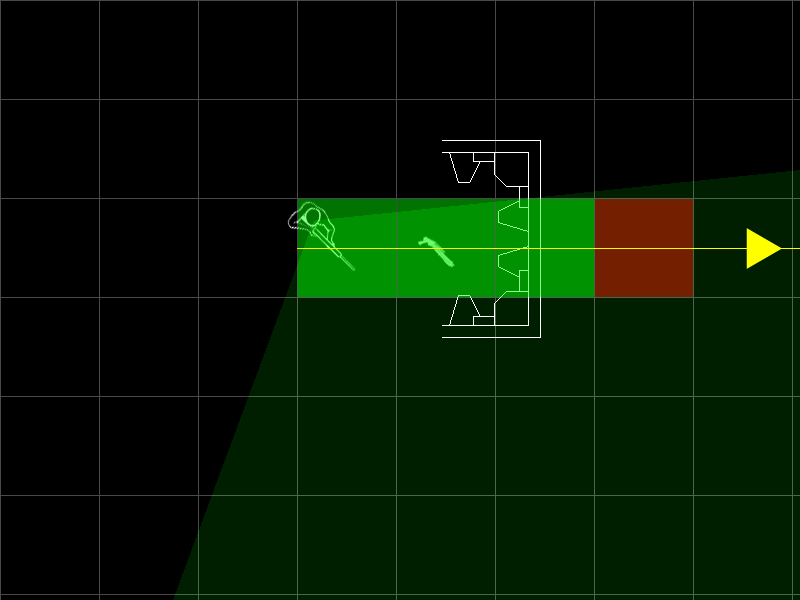
\includegraphics[width=0.75\textwidth]{Images/sceneAlgorithm/01.png}
\captionfonts
\caption[Traversing The Camera View]{A moment in time.  The objects are white to show that they are only rendered to the depth buffer at this stage.  The cells of the grid within the camera's view are being traversed.  Green represents cells visible to the camera.  Red represents occluded cells.}
\label{fig:algorithm-01}
\end{center}
\end{figure}

Now that the scene is fully traversed and all objects that are from visible cells are queued up, they get rendered with color write on.
Figure \ref{fig:algorithm-03} shows a full color scene with objects being rendered only if their cells were determined to be visible.

\begin{figure}
\begin{center}
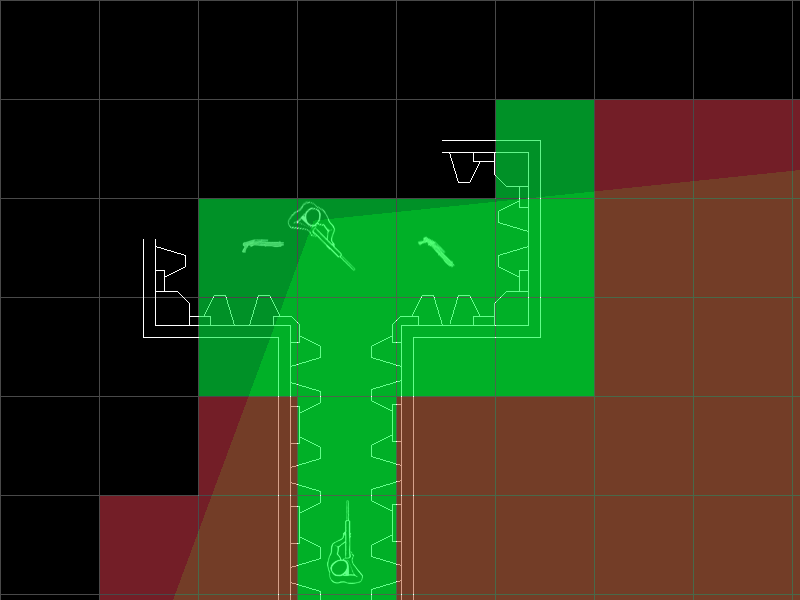
\includegraphics[width=0.75\textwidth]{Images/sceneAlgorithm/02.png}
\captionfonts
\caption[Traversed Camera View]{The scene fully traversed.}
\label{fig:algorithm-02}
\end{center}
\end{figure}

\begin{figure}
\begin{center}
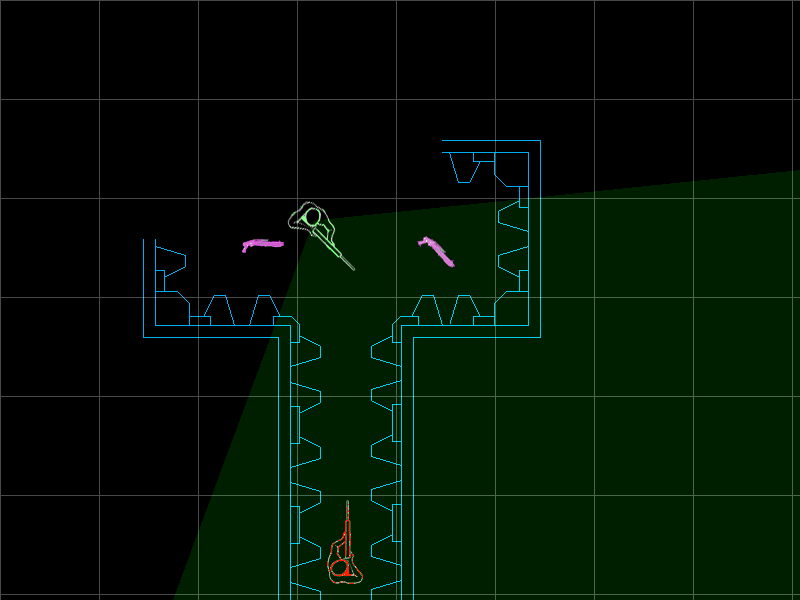
\includegraphics[width=0.75\textwidth]{Images/sceneAlgorithm/03.png}
\captionfonts
\caption[Rendered Scene]{The scene is now rendered in full color.}
\label{fig:algorithm-03}
\end{center}
\end{figure}

\section{Grid View Frustum Culling}
\label{grid-view-frustum-culling}

\subsection{Overview}
\label{Overview}
The view frustum culling occurs on the grid cells only, rather than on each individual object in the scene.
This allows all objects grouped in a cell to be culled out at once rather than making the CPU check every object individually.
If a cell is right at the border of the view frustum and a few objects inside the cell aren not in the frustum, it is not a problem to have the GPU needlessly render them.
The work done by the CPU checking all objects in a cell will cause a higher performance drop than having the GPU draw a few wasted objects.
This algorithm allows for large scenes with fine enough grids that there will usually be very few wasted objects compared to the immense number of objects that do get rendered.
The space should be subdivided by the grid in a way that renders as few wasted objects as possible.
This applies to the occlusion culling as well.
For example, if the camera is located inside a room, the cells at the border of the room should contain as few objects on the other side of the wall as possible or else a large portion of invisible objects get rendered along with the visible objects in the current room.

The cells in the grid should be traversed front to back relative to the view.
Figure \ref{fig:vf-and-occluders} shows a top down view of a scene.
Objects closer to the camera get rendered to the z buffer before objects in the back do.
Cells farther from the camera get tested against the objects in front that are potentially occluding them since they are in the z buffer.

\begin{figure}
\begin{center}
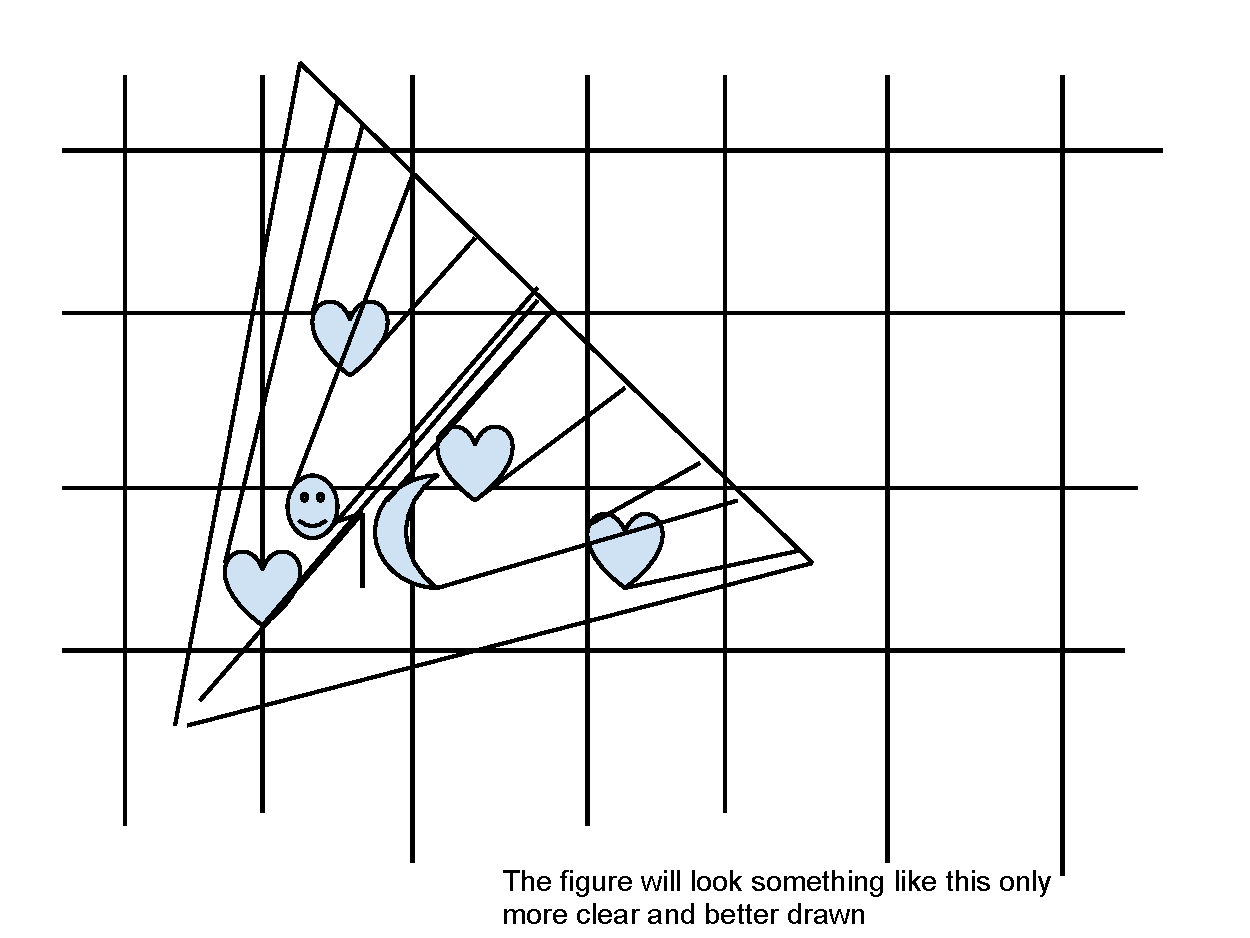
\includegraphics[width=\textwidth]{Images/frustum.pdf}
\captionfonts
\caption[View Frustum and Occluders]{A view frustum, and the objects inside occluding each other.}
\label{fig:vf-and-occluders}
\end{center}
\end{figure}

A true front to back traversal of a grid is very difficult to do well.
One attempt involved traversing out with rays from the center and stopping the traversal when reaching an occluded cell or the far plane as shown in figure \ref{fig:vf-ray-traversal}.
A 3D DDA line rasterizing algorithm would be used to traverse the cells along a ray.\cite{dda-line}
This method was rejected early on.
There was difficulty in figuring out the best way to align the rays so that duplicate cell traversals were minimized and absolutely no cells were ever missed.

\begin{figure}
\begin{center}
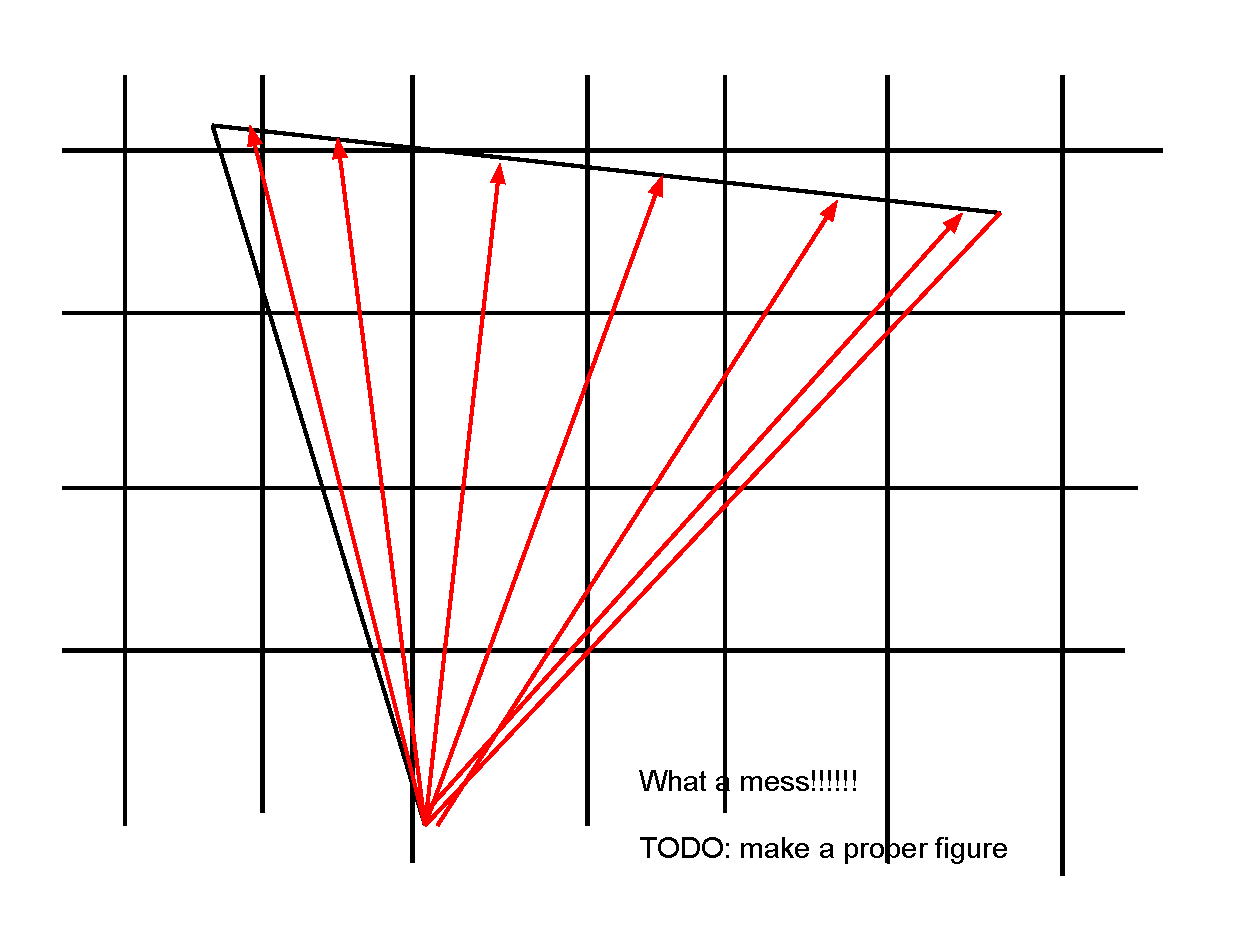
\includegraphics[width=\textwidth]{Images/ray-traversal.pdf}
\captionfonts
\caption[Ray Based Traversal]{Showing an example of ray based frustum traversal.}
\label{fig:vf-ray-traversal}
\end{center}
\end{figure}

Another method for grid traversal uses the chessboard metric.\cite{chess}
Each slice of the frustum is determined by traversing cells that are a certain grid distance away from the origin as shown in figure \ref{fig:chess-metric}.
The distance is increased by 1 each slice.
The view vector itself is rasterized as a line in 3D using the DDA algorithm.
The cells that make up the points of the rasterized line are used as origin points from where traversal should fan out for that slice.
This algorithm made it difficult to avoid traversing cells completely outside of the view frustum.
When the view is at a 45 degree angle, there is a huge space past the far plane that ends up being needlessly traversed.
Modifying the algorithm to avoid this, especially extended to 3D, was too messy.

\begin{figure}
\begin{center}
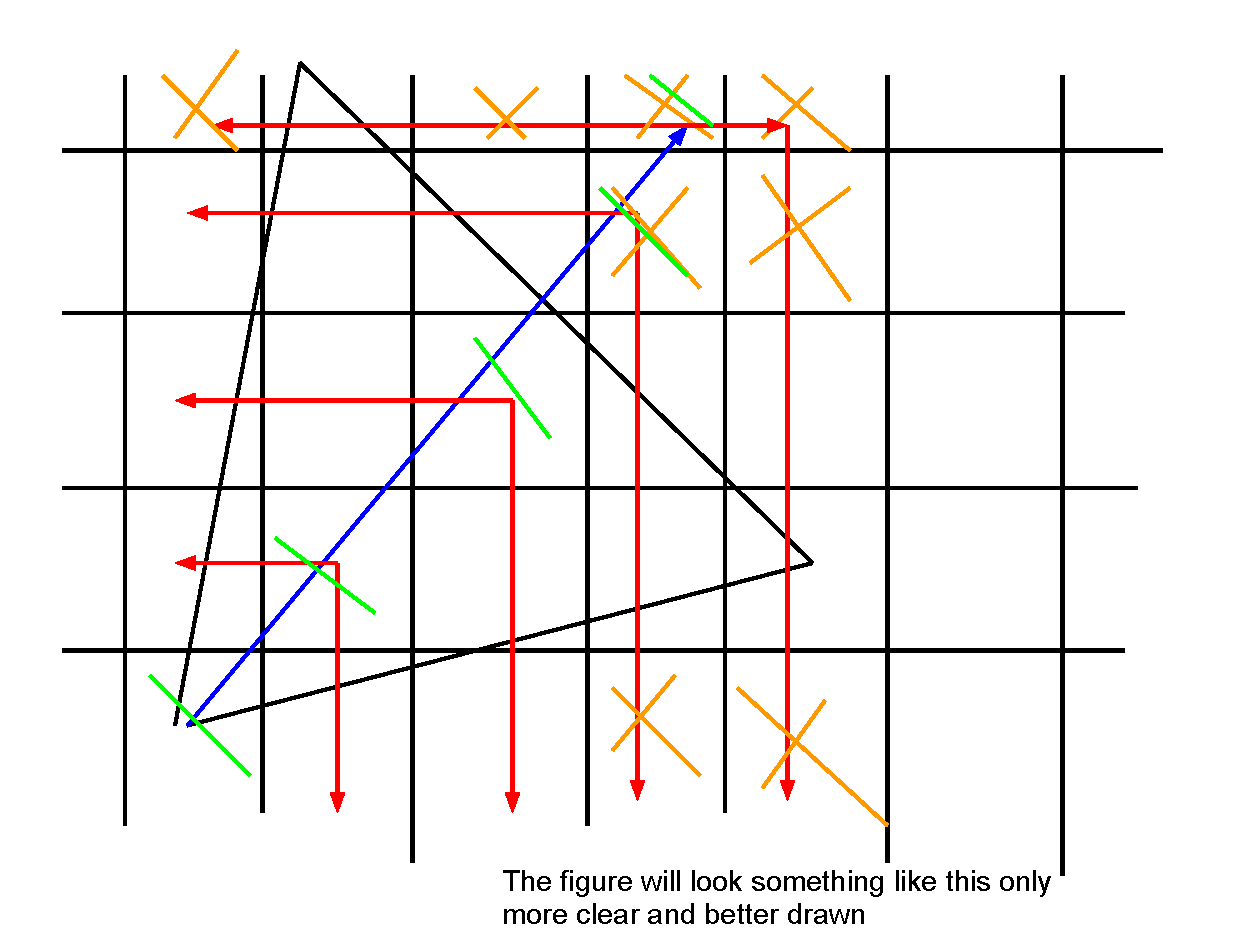
\includegraphics[width=\textwidth]{Images/chess-metric.pdf}
\captionfonts
\caption[Chessboard Metric]{The chessboard metric in action.}
\label{fig:chess-metric}
\end{center}
\end{figure}

The final idea involves taking axis aligned slices of the grid perpendicular to the highest magnitude component of the view vector.
It is a simple algorithm compared to the previously tried solutions and can be based on existing convex polygon rasterization algorithms but extended to 3D.
This is not a true front to back traversal but it provides the needed results.
In figure \ref{fig:frustum-iter}, cell 8 is traversed after cell 7, but cell 8 is closer in distance.
However, cell 7 will never occupy space in front of cell 8, so any objects in cell 7 will never be drawn in front of cell 8.
Cell 8 will be occluded by objects in cell 3 and 0, while cell 7 will most likely by occluded by objects in cells 6, 5, 2, 1, and 0.
As long as a cell is traversed after the cells that could potentially occlude it, the query results will be optimal and not create false positives.
This gives a true occlusion order traversal but not a true depth order traversal.
This same traversal order is also perfect for roughly depth sorting alpha blended objects that will need to be rendered later.
A shorter sub sort per cell rather than sorting over the entire list of objects to render can give the correct rendering order for transparent objects.
This depth sorting can even be parallelized by using a separate thread per cell, however we leave this for future work.

\begin{figure}
\begin{center}
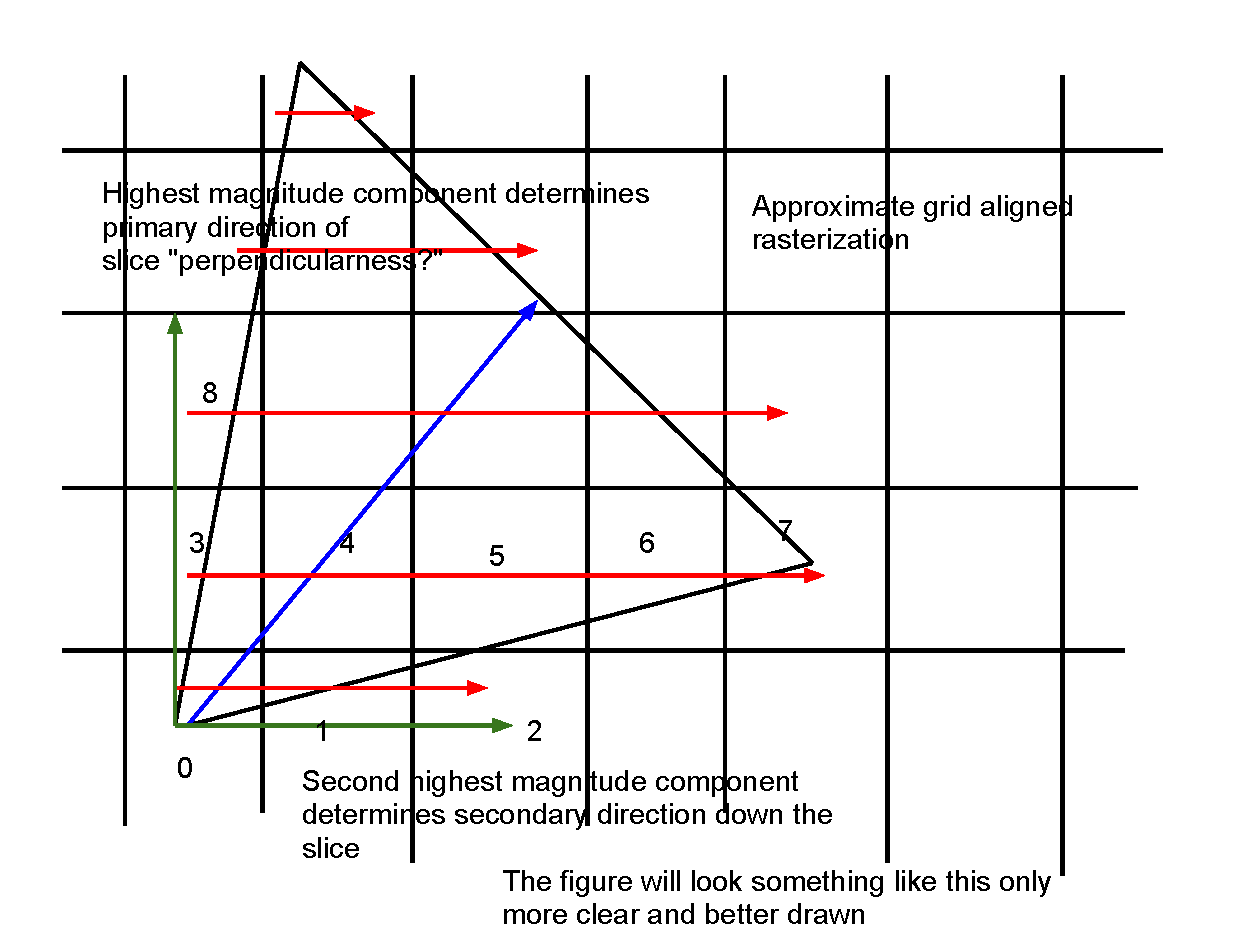
\includegraphics[width=\textwidth]{Images/frustum-iter.pdf}
\captionfonts
\caption[View Frustum Traversal]{Occlusion order traversal.}
\label{fig:frustum-iter}
\end{center}
\end{figure}

\subsection{Handling Wide Fields of View}
\label{handling-wide-fields-of-view}

In practice, view frustums are very wide.
A camera using a standard 90 degree vertical field of view on a 16:9 wide screen monitor will create a horizontal field of about 160 degrees.
Wide frustums cause cells that should have been occluded to be traversed before the cells that occlude them as shown in figure \ref{fig:wide-frustum-iter}.
In this case cell 0 is most likely occluded by cells 3, 4, and 5.
Even if the camera is staring straight at a wall, cells 0, 1, and 2 will falsely pass the occlusion queries because the wall in cell 3 hasn't been rendered to the z buffer yet.

\begin{figure}
\begin{center}
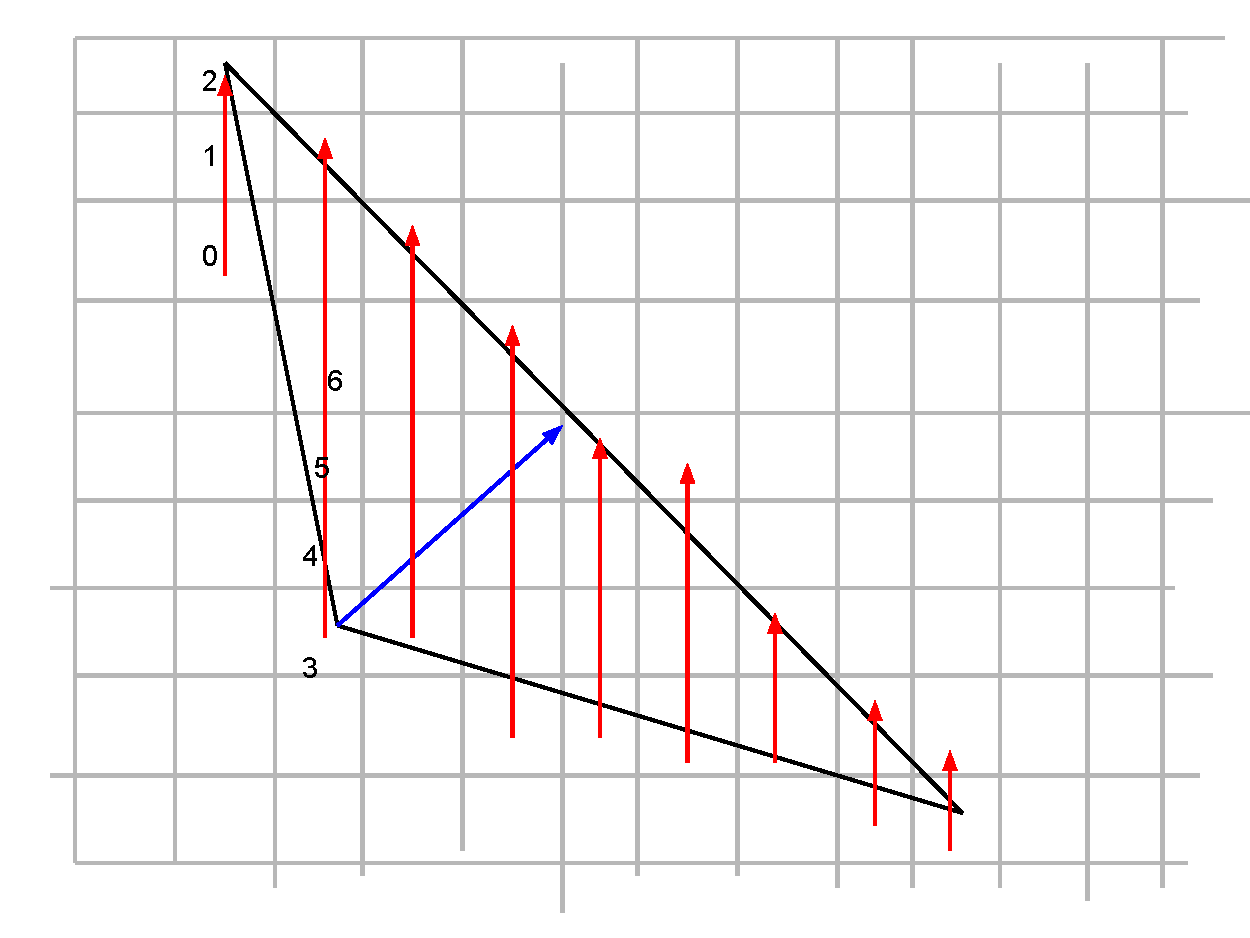
\includegraphics[width=\textwidth]{Images/wide-frustum.pdf}
\captionfonts
\caption[Incorrect Wide View Frustum Traversal]{Incorrect traversal of angled wide view frustum.}
\label{fig:wide-frustum-iter}
\end{center}
\end{figure}

Splitting the frustum into pieces solves this.
The splitting point is centered around the cell where the eye is located as shown in figure \ref{fig:correct-wide-frustum-iter}.
This creates new convex volumes out of the split view frustum.
In 3D, the frustum is split into 8 pieces by the x, y, and z planes.
A convex polygon plane clipping algorithm will do the trick.
The volumes are now traversed in a fan out order around the center cell.
In the figure below, first the central volume is traversed, and then cells 22, 23, and 24 are traversed afterwards.
This keeps the correct occluder order prevents cells from being falseley determined to be visible.

\begin{figure}
\begin{center}
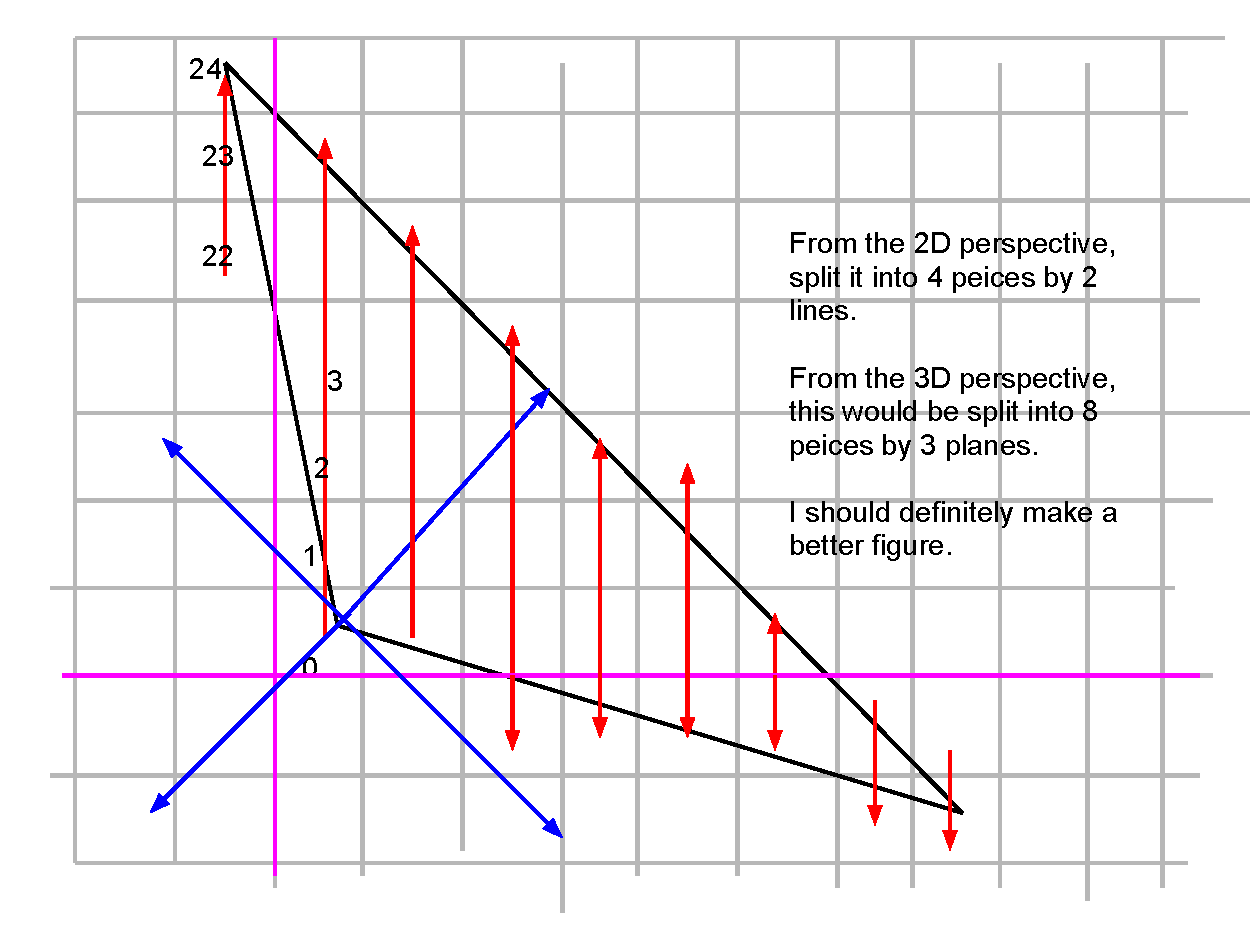
\includegraphics[width=\textwidth]{Images/wide-traversal.pdf}
\captionfonts
\caption[Corret Wide View Frustum]{Correct traversal of split angled wide view frustum.}
\label{fig:correct-wide-frustum-iter}
\end{center}
\end{figure}

\subsection{Objects at Cell Boundaries}
\label{objects-at-cell-boundaries}
When doing spatial queries against a grid, some group of cells gets traversed and all objects in those cells get returned in the query.
If an object occupies multiple cells it can potentially get added multiple times as a query result.
Keeping track of a 64 bit unsigned query id counter can prevent this.
The main scene can store a query counter, and increment it every time a query occurs.
The objects returned by the query can keep a query counter within them as well.
If the object's counter is less than the scene's counter, then the object has not been added to the query results yet.
As the object is added, its counter is set to the scene's counter and any other cells that contain the object will not needlessly duplicate the object in the query.

In a multithreaded engine, when many queries can occur in parallel, a lockless set of query ids per object can work.
If a query id is already in the object's query set, the object can be ignored.
After the query results are done, the query id can be removed from the set, keeping the set from growing.
Lockless sets that are part of Intel Thread Building Blocks do not allow safe lockless removal, so it may be best to clear these sets at some synchronization point such as the end of a frame to prevent them from growing too large.\cite{tbb}

\subsection{The Rasterizing Algorithm}
\label{the-rasterizing-algorithm}
The algorithm does nt handle just frustums, but any convex polygon with any arbitrary amount of points and edges.
This allows the algorithm to handle the frustum being clipped against the level bounds and sliced into 8 peices to handle wide and angled views.

The algorithm is optimized enough that it is able to quickly process very dense grids.
It has been tested on grids of 1,000 x 1,000 x 1,000 cells and the framerate stayed at about 40 FPS in the worst case, and at about 100 in other cases.
It was tested by making OpenGL render a point at the center of what would be a cell in 3D space.
Such a dense grid is not practical for the visibility culling algorithm itself.
It would take over 59 gigabytes in RAM to store one billion 64 bit NULL pointers for a completely empty scene.
Since the hardware must also render a box for each cell, the performance would drop siginificantly rendering that many boxes and later retreiving occlusion query results even if a system had that much memory.
Thus, the CPU is able to rasterize dense grids with relative ease, while memory and GPU power are the bottlenecks requiring the grids to be even less dense in practice.

It is possible to avoid implementing this algorithm and use a simpler axis aligned box rasterizer.
The axis aligned bounding box of the view frutum can be traversed in occlusion order row by row by just using three nested loops, one for each dimension.
In this case cells that are outside of the view frustum get traversed, creating some wasted effort by the CPU as well as requiring either wasted cell queries or to check if each cell is in the view frustum.

The algorithm works by taking a convex polygon as shown in Figure \ref{fig:scene-frust} and processing it slice by slice down the grid as shown in Figure \ref{fig:scene-frust-slice}.
Each slice is now a 2D polygon, so a modified 2D rasterizer is used similar to existing 2D convex polygon rasterizing algorithms.
For each row in the slice, the range of cells to be traversed is computed as shown in Figure \ref{fig:scene-frust-row}.
The full implementation is presented in the appendix.

\begin{figure}
\begin{center}
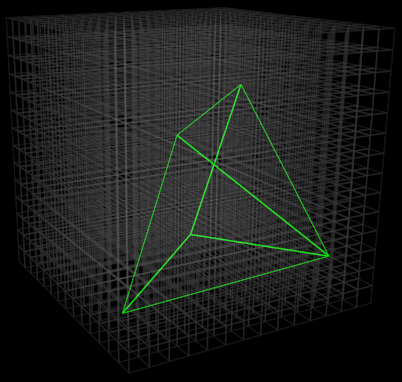
\includegraphics[width=0.5\textwidth]{Images/RasterizingAlgorithm/Final/Frust.png}
\captionfonts
\caption[A Frustum]{A view frustum within the bounds of a scene.}
\label{fig:scene-frust}
\end{center}
\end{figure}

\begin{figure}
\begin{center}
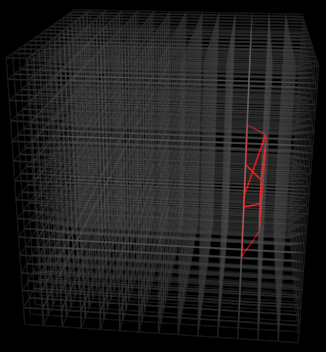
\includegraphics[width=0.5\textwidth]{Images/RasterizingAlgorithm/Final/FrustSlice.png}
\captionfonts
\caption[A Frustum Slice]{A 2D slice of the same frustum seen from the side.}
\label{fig:scene-frust-slice}
\end{center}
\end{figure}

\begin{figure}
\begin{center}
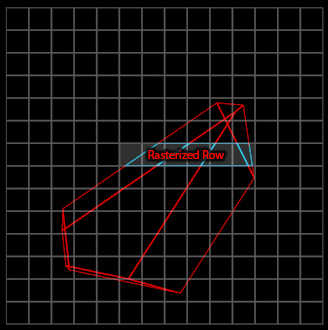
\includegraphics[width=0.5\textwidth]{Images/RasterizingAlgorithm/Final/FrustSliceNRowOrthoLabeled.png}
\captionfonts
\caption[A Frustum Slice And Row]{A row from the slice being rasterized.}
\label{fig:scene-frust-row}
\end{center}
\end{figure}

\section{Rendering}
\label{rendering}

\subsection{Render State Sorting}
\label {render-state-sorting}
Other rendering algorithms that make use of hardware occlusion queries usually benefit from having all objects sorted front to back.
In Figure \ref{fig:a-scene} Tree A should be drawn before the Tank since it can potentially occlude the tank.
After that the Person should be tested against the Tank and Tree A.
Then Tree B gets tested against everything else.
This would require the objects to be drawn in the order, Tree A, Tank, Person, Tree B.

\begin{figure}
\begin{center}
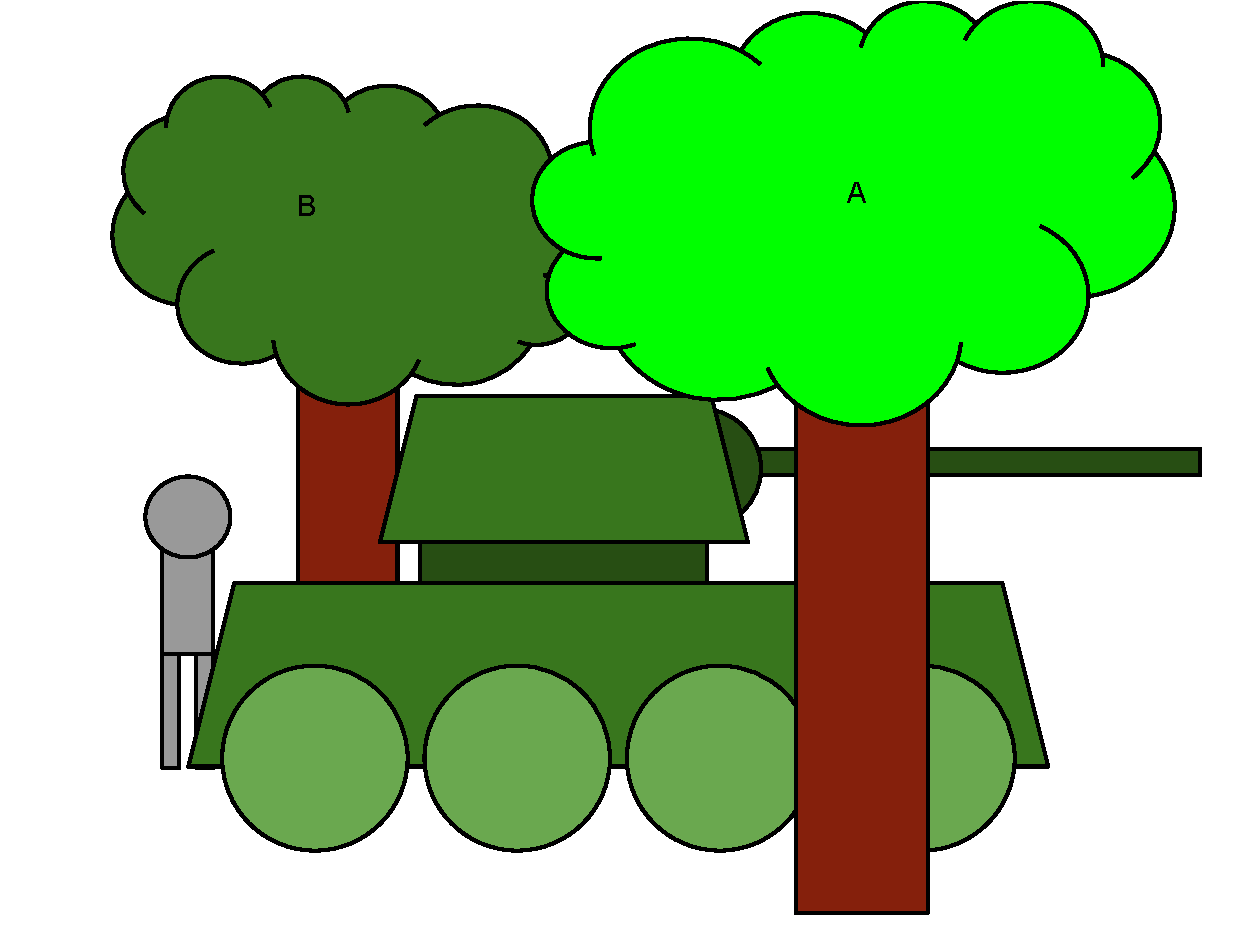
\includegraphics[width=0.75\textwidth]{Images/sample-scene.pdf}
\captionfonts
\caption[A scene]{A scene.}
\label{fig:a-scene}
\end{center}
\end{figure}

Rendering performance would suffer since these objects are not sorted in an optimal render state order, but in occlusion order.
When rendering a large number of objects, they should be sorted in a way that causes the least amount of change in the render state.
It would be better to render Tree A, Tree B, then switch to the shader and textures that render the tank, then do the same for the person.
The algorithm in this paper avoids this problem and allows objects to be queued up and then sorted by their render state.

The renderer used for this project sorts objects first by shader, then textures, then by the instance of mesh.
This is done in order of which changes cause the worst performance hit for the GPU.\cite{d3d10-sys}
It should also be possible to quickly depth sort the meshes being rendered to avoid some overdraw but the objects are already sorted well enough when the view frustum is rasterized front to back.
True depth sort is only needed for alpha blended objects.

\subsection {The Visibility Culling / Depth Pass}
\label{the-visibility-culling-depth-pass}

The first phase involves performing a depth pre pass while performing the occlusion queries.
The depth pre pass renders solid objects to the z buffer with color writing disabled so the complex pixel shaders that compute lighting and color are not run.
This is used for the occlusion queries during this stage as well as for preventing pixel shader overdraw later.
For each unoccluded cell that is traversed during this phase, its objects are rendered to the z buffer as well as being added to the main render queue.

First, the query results from last frame are gathered.
This updates the visibility status of cells for the current frame.
Since the cell query results are used next frame, objects may pop in a frame late.
This is unnoticeable at high frame rates due to how little time this takes, and is a common sacrifice other engines make when using occlusion queries.
This is the part of the algorithm that takes up about 25\% CPU time.
Query results may take upto four frames to be ready in some cases, so even using the results next frame rather than the current frame causes a CPU stall.
The frame rate still remains high, sometimes reaching 300 FPS if running only queries but not rendering anything.
The call to retrieve the query result blocks the CPU until the result is available, but it is possible to first check if the result is available before making the blocking call.
This is avoided to keep the algorithm simpler and avoid rendering frames where the object is not visible yet.
This stall can be inconsequential if a separate thread retrieves the query results while the engine is left to run Physics, AI, sound, and other subsystems.

The cells keep track of their last visible frame by storing a 64 bit unsigned frame counter.
A 64 bit unsigned integer can store more atoms than there are in the universe.
Even if the renderer is running at 500 FPS, it will take 15,768,000,000 years for this counter to roll over.
The scene itself keeps track of the current frame counter in its own 64 bit unsigned integer.
When a cell query is retrieved, it writes the current frame counter of the scene as the last visible frame.
This way it's unnecessary to to iterate over all cells every frame to reset their visibility status.

\begin{lstlisting}
//TODO: fix this
isCellVisibleLastFrame()
	return cell.lastVisibleFrame == scene.currentFrame - 1;
\end{lstlisting}

In order to prevent too much work during the depth pre pass, the artists can specify how the object should be rendered during this phase.
This is one of the only settings artists need to tweak in the environment to push a little extra performance.
The three settings for an object are to always render, sometimes render, and to never render.
An object can be marked as an essential occluder that must always be rendered if its cell is visible.
This is for objects like walls, terrain, or any other objects that keep the world water-tight.
These are objects that must populate the z buffer in order for cells behind to be properly occluded.
The second setting of "sometimes" is reserved for fairly large detail adding objects that would be in the middle of rooms, such as crates, columns, or trees.
The deferred renderer in the game Space Marine limits the depth pre pass to only 75 objects in order to prevent too much work during this phase. %(http://www.slideshare.net/blindrenderer/rendering-tech-of-space-marinekgc-2011)  
This engine only adds objects marked to render sometimes if there are not already 75 objects rendered in the depth pass.
Since the scene is traversed front to back, the objects close to the camera and likely to contribute to occlusion usually make it while the further away objects are avoided.
The third setting of "never" is for the tiny objects that add detail.
In a fully detailed environment it is likely that there will be very many of these objects.
They are likely to not contribute much to the occlusion and rendering them during this phase can be a waste.

\begin{figure}
\begin{center}
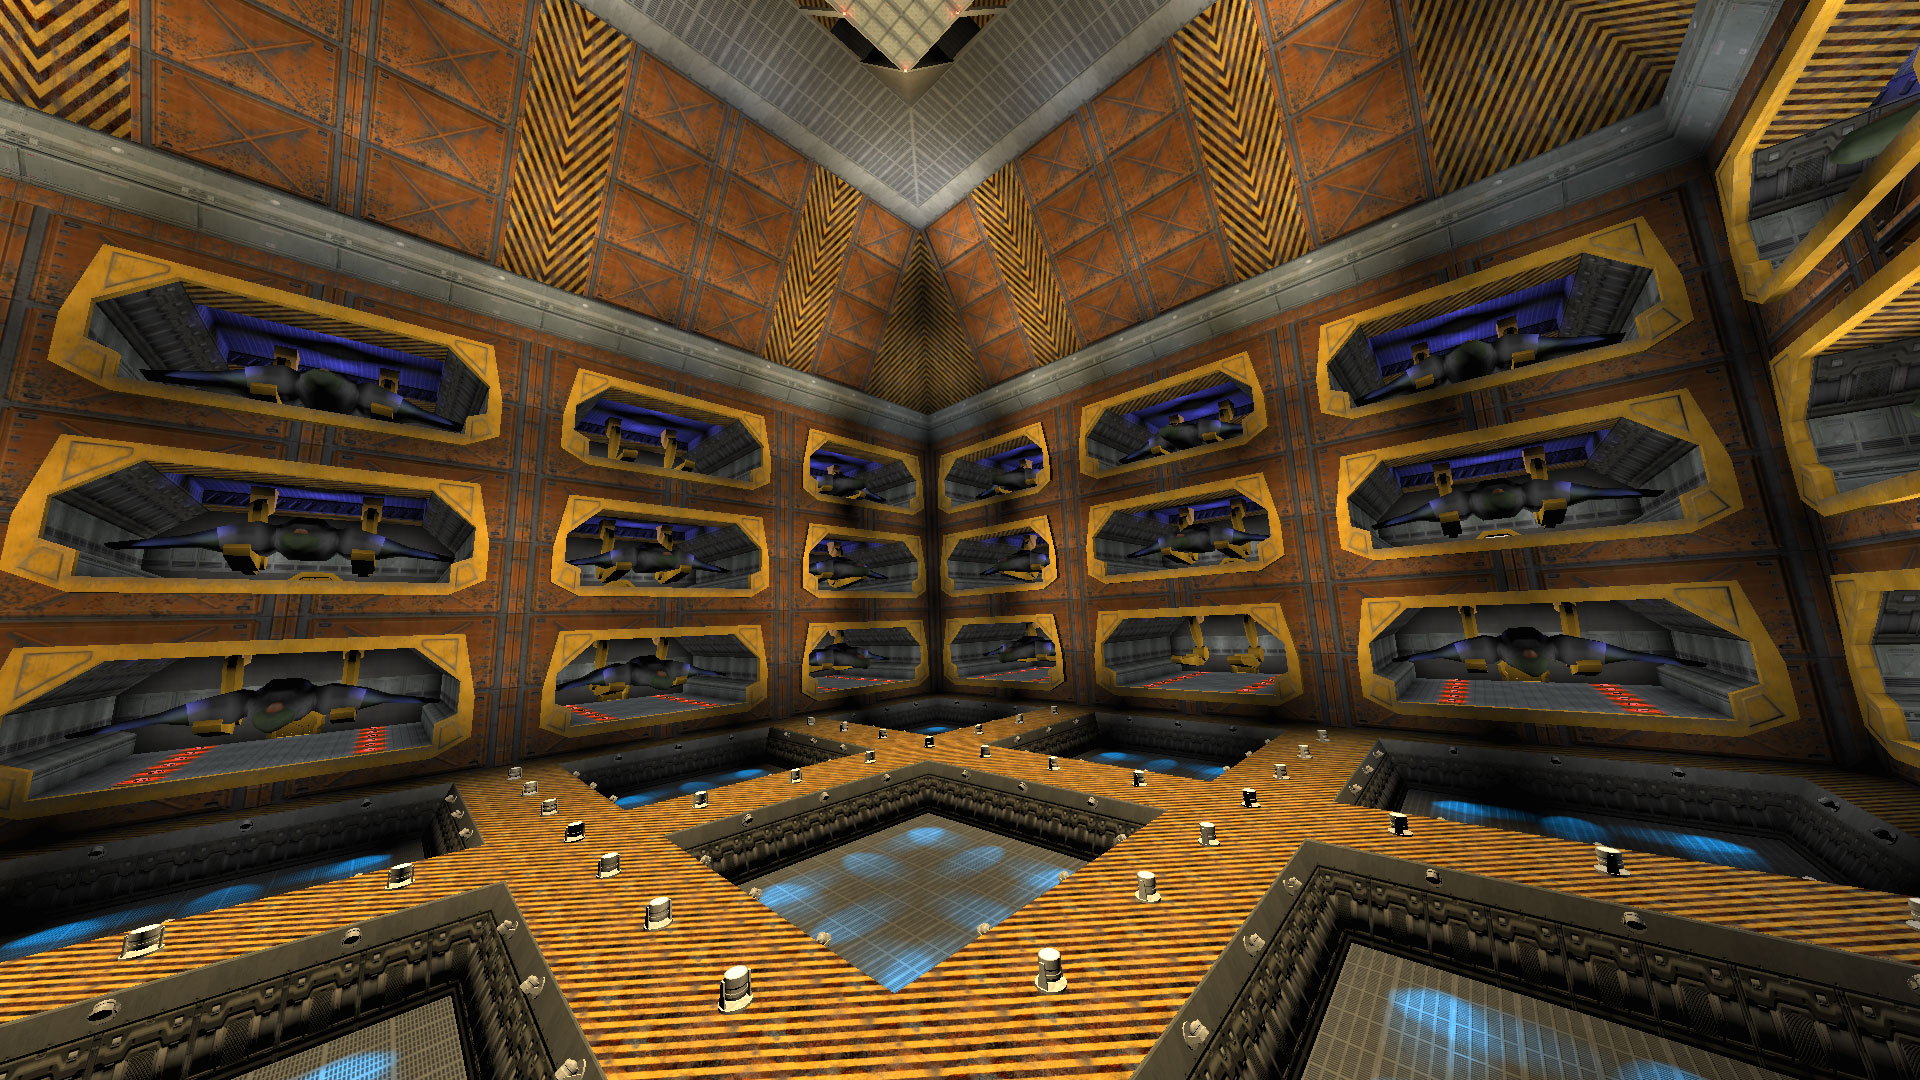
\includegraphics[width=\textwidth]{Images/HangarCorner.jpg}
\captionfonts
\caption[Hangar Corner]{Hangar corner}
\label{fig:hangar-corner}
\end{center}
\end{figure}

In figure \ref{fig:hangar-corner} the walls, ceiling, and floors are marked to always render.
The fighter jets inside the hangars are marked to sometimes render.
The lamps on the floor and clamps holding the jets in place are marked to never render.

\begin{figure}
\begin{center}
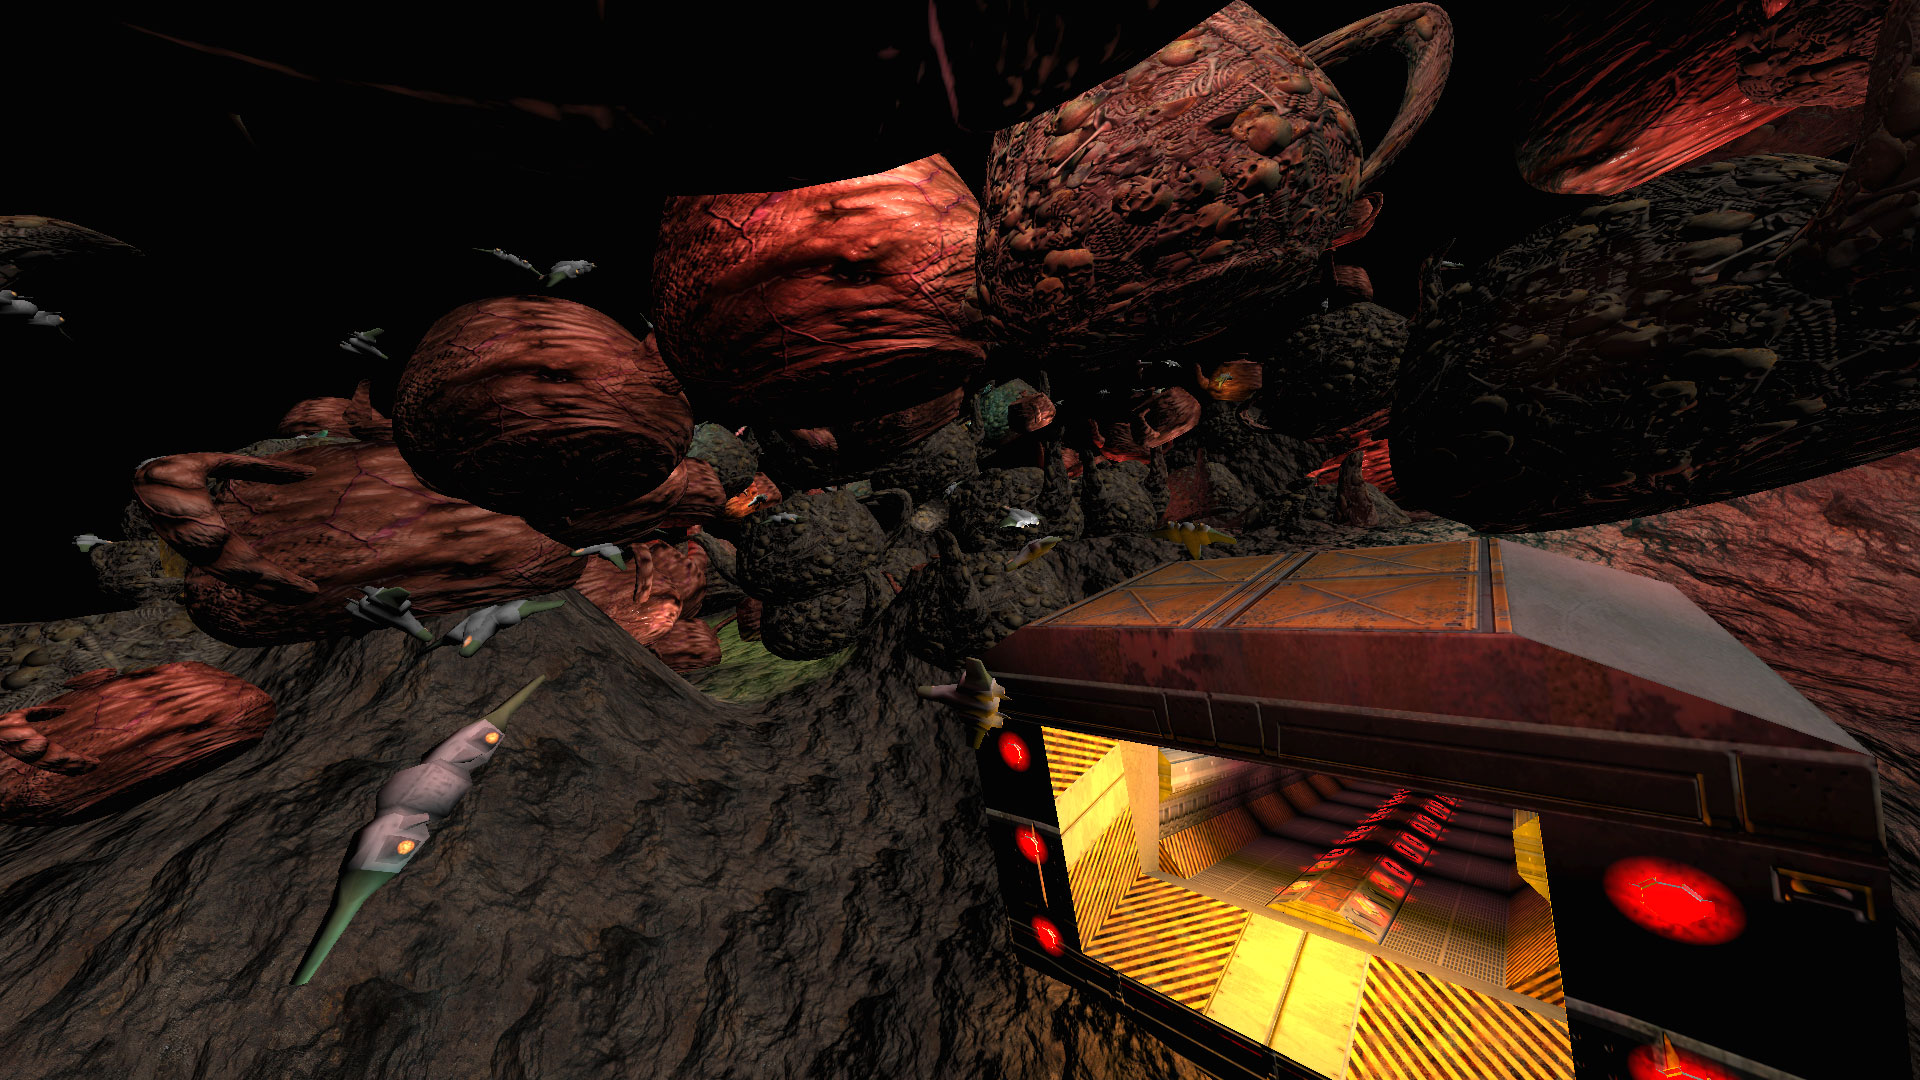
\includegraphics[width=\textwidth]{Images/HangarEntrance.jpg}
\captionfonts
\caption[Hangar Entrance]{Hangar entrance}
\label{fig:hangar-entrance_}
\end{center}
\end{figure}

In the outdoor area of figure \ref{fig:hangar-entrance_}, The building, underground tunnel walls, and the terrain are set to always render.
The teapots and jets are set to sometimes render.
The red lamps on the building are set to never render.

The following pseudocode shows the algorithm.

\begin{lstlisting}
//TODO: make this be some C++ and make it fit horizintally properly
uint64_t frameCounter

//retreive cell queries from last frame
for each query from last frame
	get query result
	if any samples passed
		mark cell as visible for frameCounter

++frameCounter

disable blend
//we don’t need to write colors in this phase, just populate the z buffer
disable color write
enable depth test
depth func less
set cull face to back
						
for each grid cell traversed
	if cell is not empty

disable face cull
		disable depth write
		
//cell is completely invisible, but still tested in queries			
		begin occlusion query
		draw cell
		end occlusion query			
	
if cell was marked visible during frameCounter - 1				
			for each node in cell
				add node to render queue

				if node has a solid unblended material
					if node marked to always render 
or (sometimes render and numRenderedDepthPass < 75)
						add node to depth pass queue
	
			//now that we are drawing the objects, reenable depth write
			enable depth write
			enable face culling
			
			sort depth pass queue by shader, some textures, and mesh
			//if using displacement maps, those will be needed during this phase
			//diffuse, normal, specular maps, etc... not needed here

			begin conditional render using cell query			
				for each mesh in depth pass queue
					draw mesh				
				end conditional render from cell query

			clear depth pass queue
\end{lstlisting}


\subsection {The Rendering}
\label{the-rendering}

Now all objects from cells marked as visible in the previous frame are gathered up and ready to be rendered in color.
They should be sorted by render state as mentioned earlier.
A deferred shading renderer is used for this project, but any kind of renderer can be used.
In this case, solid objects are all queued up in one render state list.
This is a great opportunity to use the batching API available on modern graphics cards to reduce draw calls and render all objects of one type in 1 call.
The depth write and depth test should still be enabled at this time since not all objects were added to the z buffer during the depth pre pass.
The depth test function should be set to less than or equal.  All lights to be rendered during the lighting pass are queued up in another list.
Transparent objects can be queued up in another list in the occlusion order mentioned earlier and rendered using forward rendering.
The same grid that stores objects in the scene can be queried for which lights affect objects to be rendered during forward rendering.

\subsection {Spreading Queries}
\label{spreading-queries}

Tight detailed indoor environments benefit from the scene using a finer grid.
The hallway in \ref{fig:hangar-halls} is built around the hangar pictured in \ref{fig:hangar-bay}.
If the grid is too sparse, large chunks of the hangar get rendered that should be occluded by the walls of the hallway because the cells are too big and contain too many objects.

\begin{figure}
\begin{center}
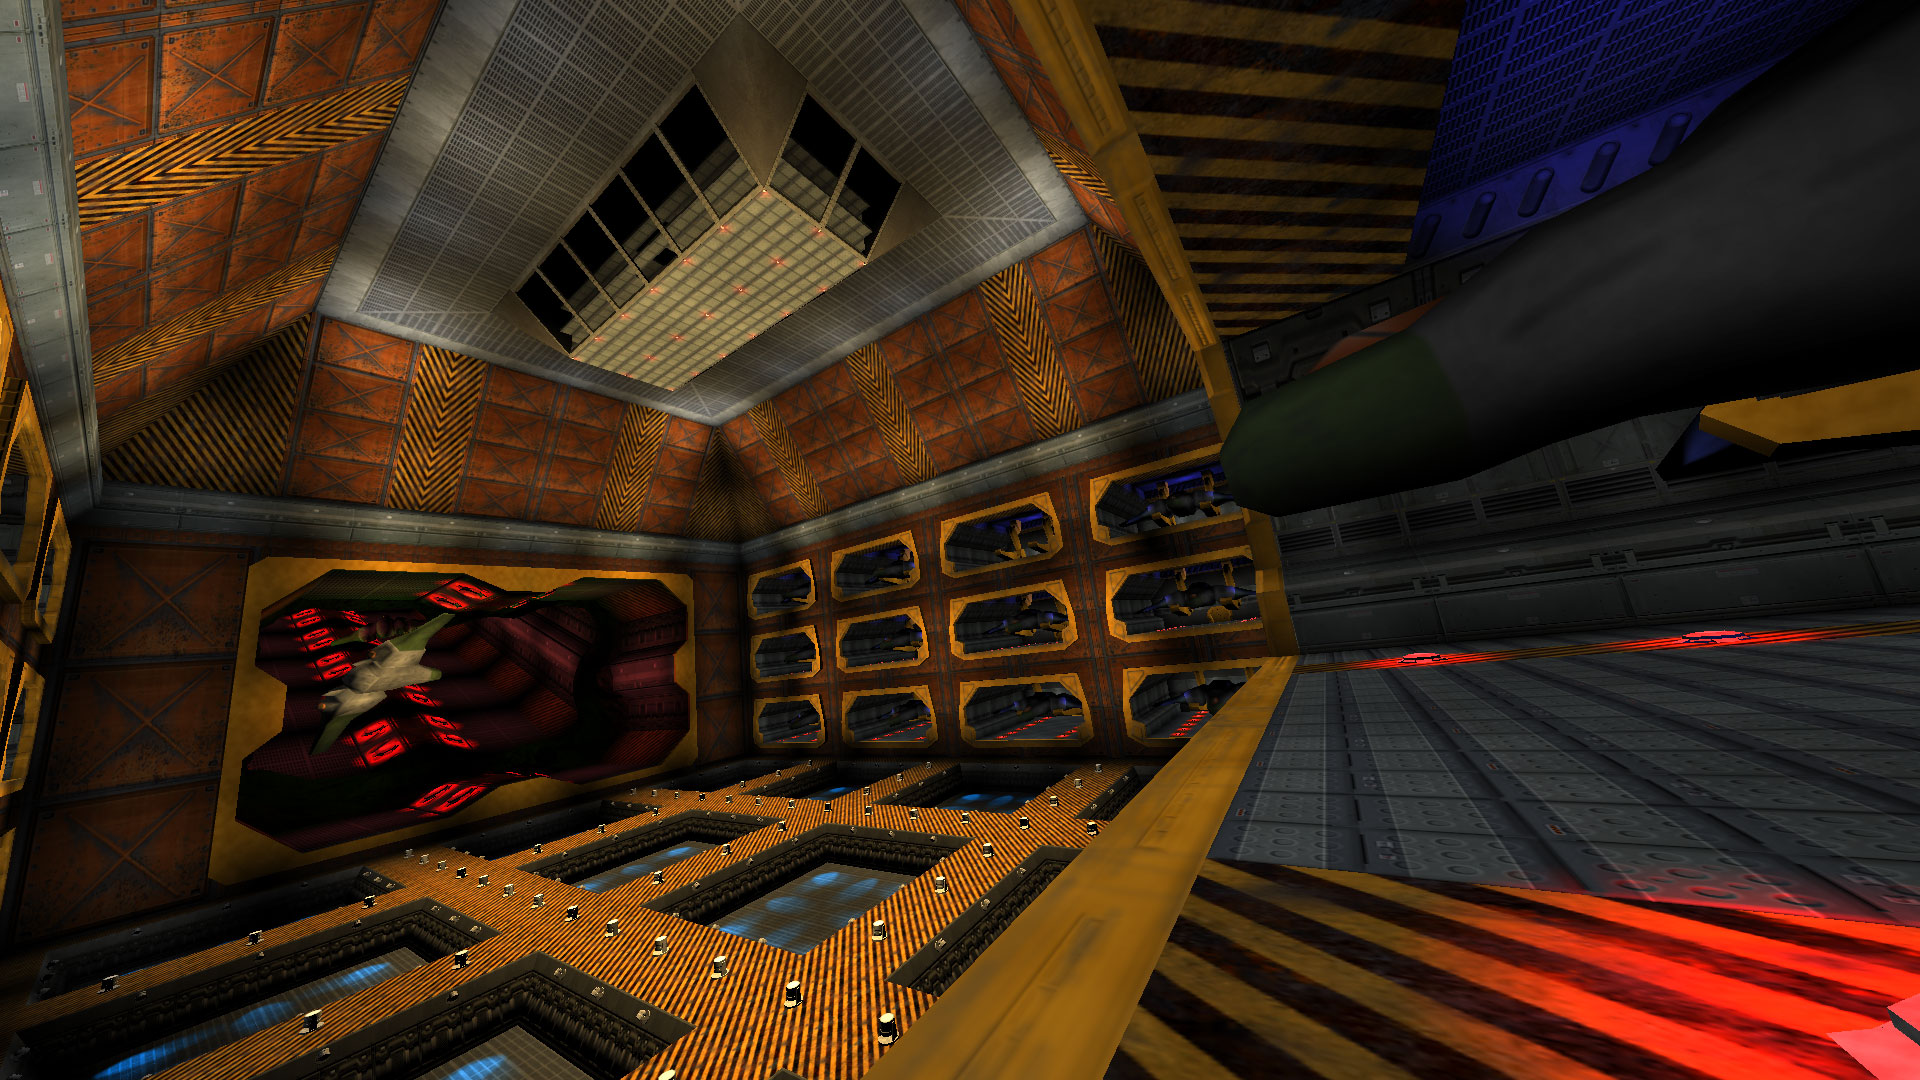
\includegraphics[width=\textwidth]{Images/Hangar.jpg}
\captionfonts
\caption[Hangar Bay]{Hangar halls}
\label{fig:hangar-bay}
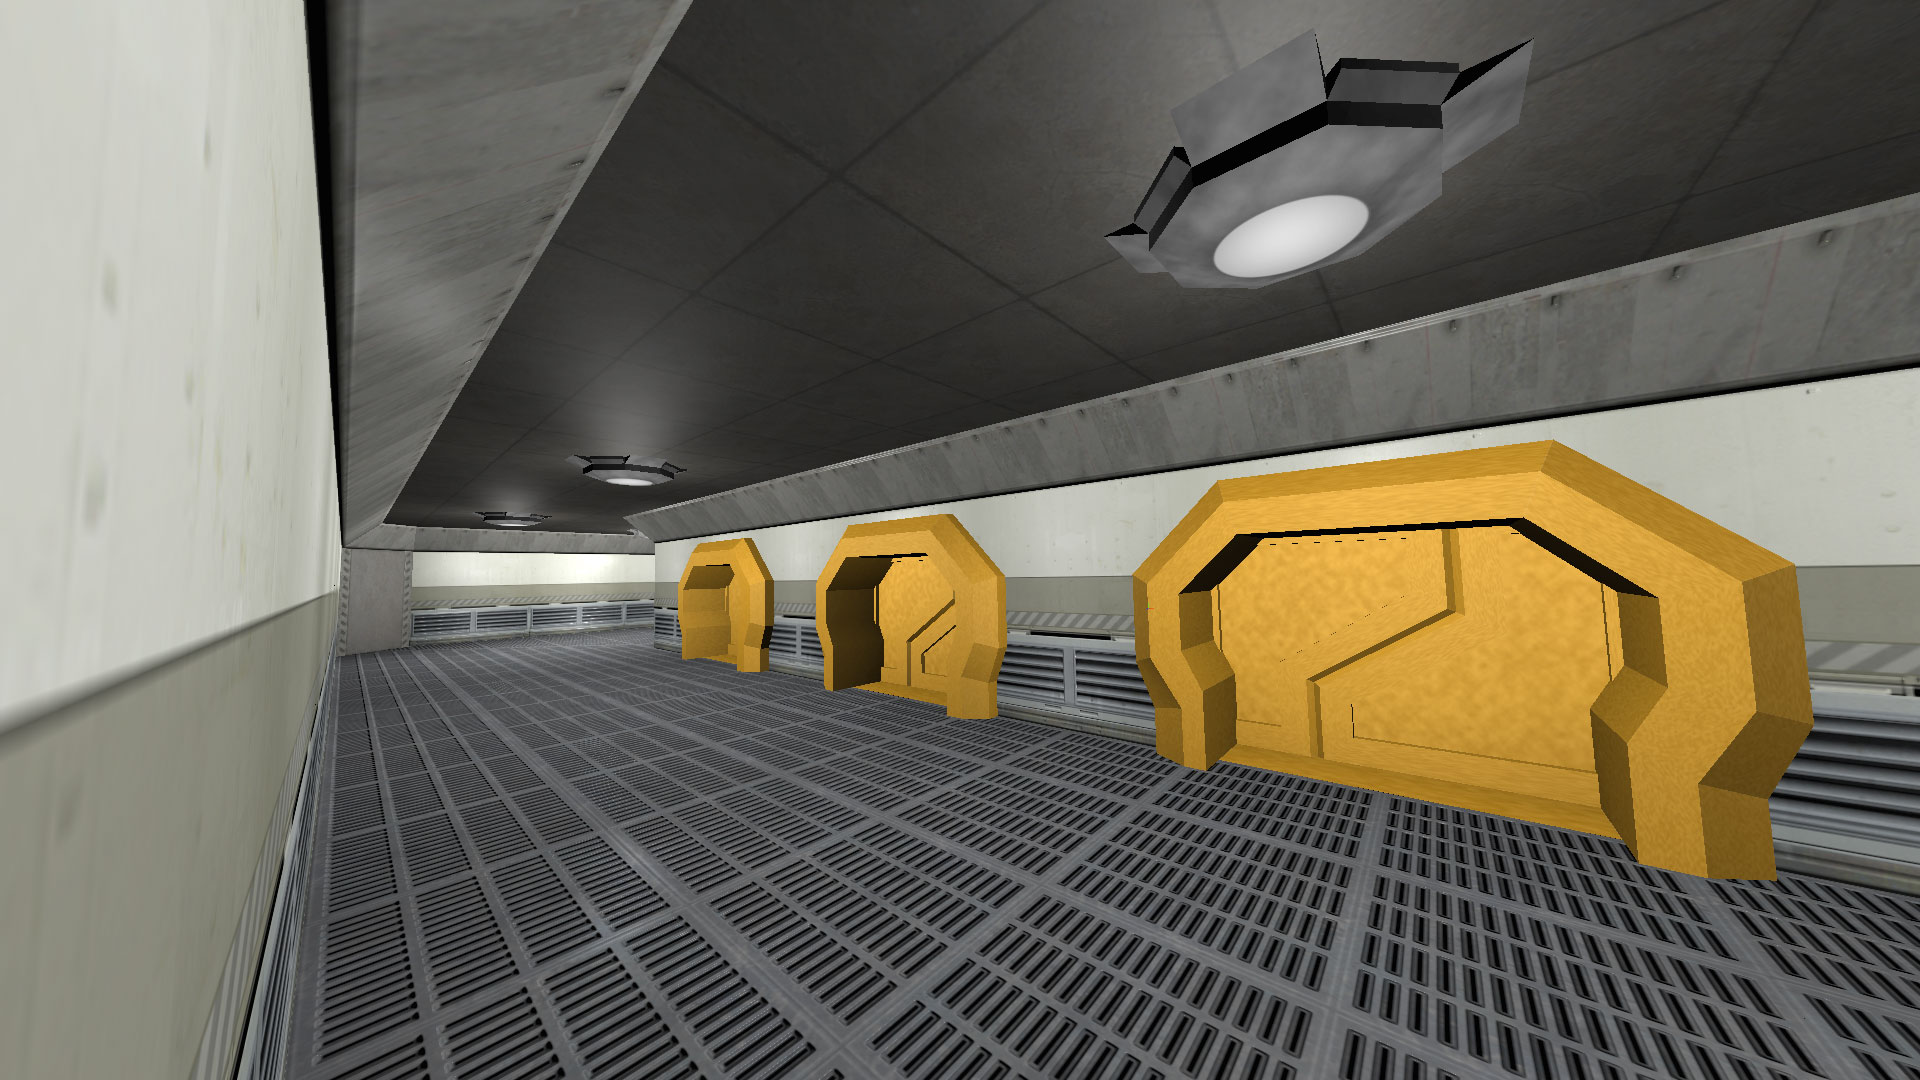
\includegraphics[width=\textwidth]{Images/HallCorner.jpg}
\captionfonts
\caption[Hangar Halls]{Hangar halls}
\label{fig:hangar-halls}
\end{center}
\end{figure}

When inside the hallway of \ref{fig:hangar-halls}, the frame rate is about 60 FPS with a fine grid, and can drop down to 25 FPS with a more sparse grid.
However, having too fine a grid can also be bad for performance overall.
The frustum rasterization algorithm has no problem with traversing grids as large as 1000 x 1000 x 1000 cells.
The querying and rendering of individual cells is the bottleneck.
Depending on the camera position and viewing angle, the number of traversed cells in a fine grid can range from about 500 to 60,000.
There is not a good way to batch all of the cubes that get rendered for the cell queries into a single draw call.
The queries happen in between rendering a group of objects to the depth buffer and there seems to be no way to have a query for each individual object in a batch at the moment.
In the worst case, that many draw calls being made causes severe performance drops down to about 4 FPS.

One solution is to try to group far away cells into one query.
It may be possible to modify the frustum rasterizing algorithm to support this in the future.
The grid could be rasterized more like a hierarchical octree.
Any far way grouped cells that are visible can then be subdivided into finer cells in later frames to filter out the portions of the scene that are not visible.
This would take considerable effort due to the way the rasterizing algorithm is currently built to traverse row by row in the grid.
A simpler solution is to limit the number of queries per frame.
A limit of about 3000 to 4000 produces good results.
Query results now need to last multiple frames.
The algorithm is becoming similar to the Coherent Hierarchical Culling algorithm, in that results of queries are likely to not change too much between frames that are close by in time. 
The current algorithm allows successful visibility queries to last for about 30 frames and failed invisible cell queries to last about 2 frames.
A lower number for invisible cells is needed to avoid waiting too long to let previously invisible cells to have their objects pop in noticeably while moving through the scene.
Now if a query result is still valid, the cell does not need to be re-queried and cells that have not been queried in previous frames have a chance.
This can at cause slightly more noticeable pop in of objects while moving since some cells get queried a few frames later at the cost of keeping the frame rate higher as shown in \ref{fig:hall-doorway}.
The frame rate being high reduces the real time it takes for an object to pop in, making it less noticeable anyway, so this tends to be a good tradeoff.

\begin{figure}
\begin{center}
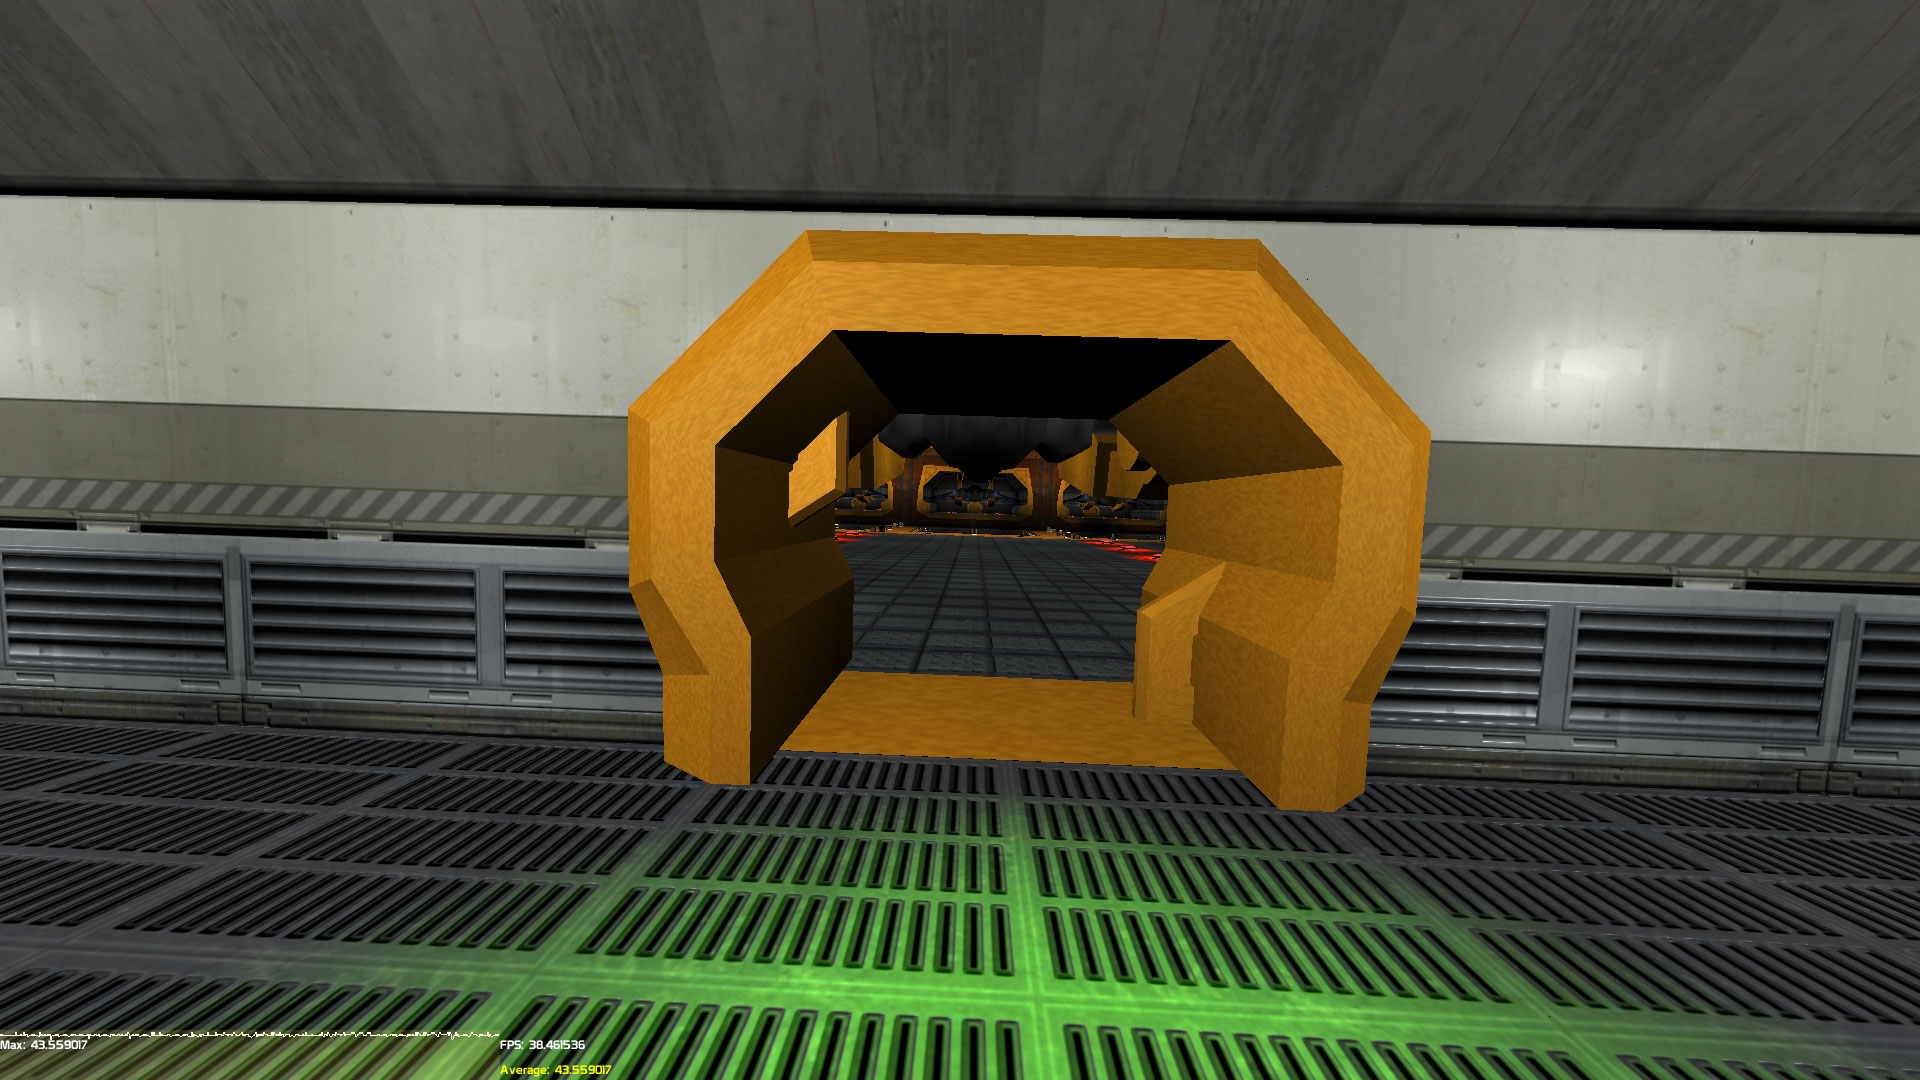
\includegraphics[width=\textwidth]{Images/HallDoorway.jpg}
\captionfonts
\caption[Hall Doorway]{Moving sideways can make far away objects seen through the door sometimes appear to pop in visibly if someone is really paying attention.
A high frame rate and an action packed game help ensure this artifact is hard to notice.}
\label{fig:hall-doorway}
\end{center}
\end{figure}

\subsection {Query Starvation}
\label{query-starvation}

When a large amount of cells needs to be queried, some cells never have a chance and patches of the world go missing \ref{fig:missing-patches}.
Cells early in the frustum traversal whose query results have expired eat up the queries that farther away cells need to become visible.
If 40,000 cells need to be queried, and nonvisible cell results last only 2 frames, those same nonvisible cells will keep executing queries.

\begin{figure}
\begin{center}
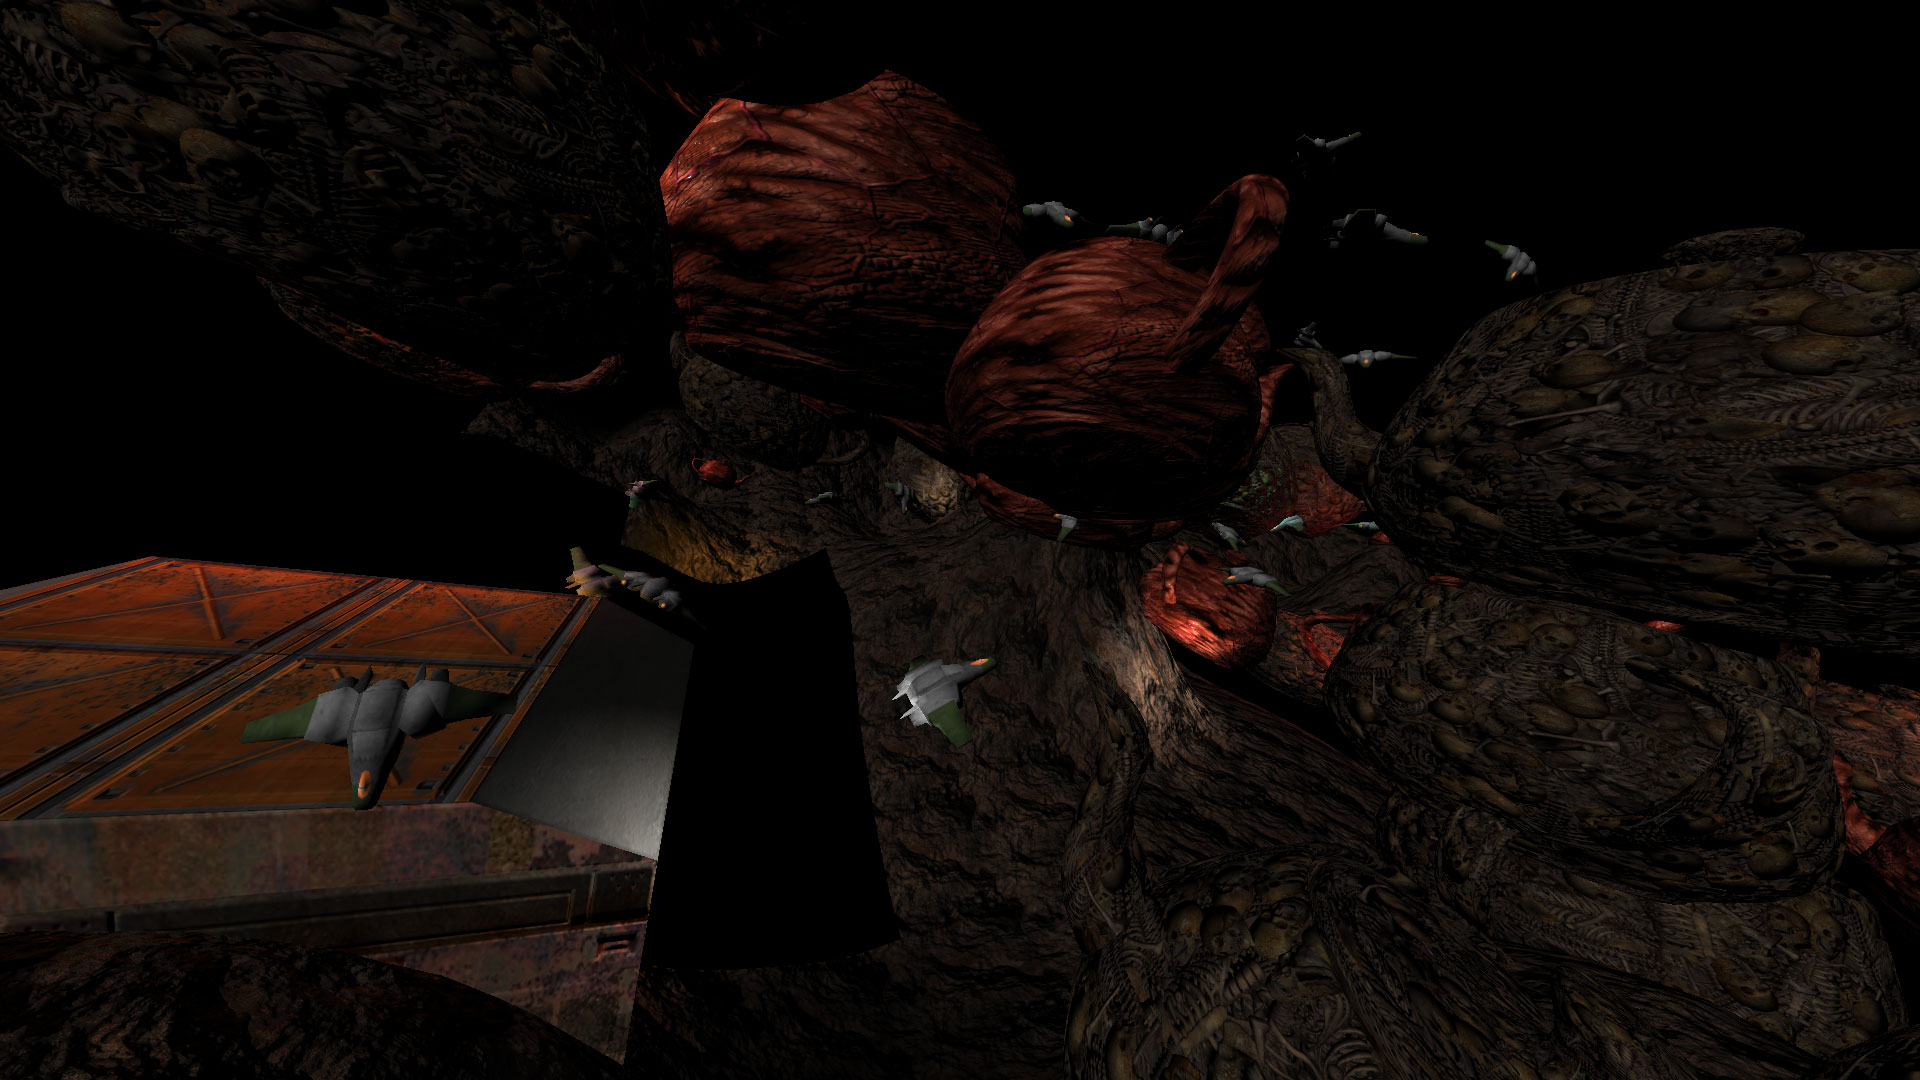
\includegraphics[width=\textwidth]{Images/MissingPatches.jpg}
\captionfonts
\caption[Missing patches]{Missing patches}
\label{fig:missing-patches}
\end{center}
\end{figure}

Extending the duration of query results when the query cap is hit, as well as offsetting the duration by a random amount, helps avoid the problem of query starvation.
It is possible to keep track of how many frames in a row have hit the query cap and base the duration extension on this amount.
After a few frames, all cells that should be visible have had a chance to be queried and the scene looks correct.
The popping artifacts stay relatively unnoticeable.

The following pseudocode shows how the current implementation takes into account the number of frames in a row the query cap was hit.  The invisibilityDurationGrowth variable should be smaller than the visibilityDurationGrowth variable to keep the previously described popping artifacts at a minimum while moving.

\begin{lstlisting}
//TODO: fix this code
for each query from last frame
	get query result
	if any samples passed
		mark cell as visible for frameCounter + (visibilityDuration + visibilityDurationGrowth * numFramesOverflowed) + rand(0, numFramesOverflowed * 2);
	else
		mark cell as invisible for frameCounter + (invisibilityDuration + invisibilityDurationGrowth * numFramesOverflowed) + rand(0, numFramesOverflowed * 2);
++frameCounter
\end{lstlisting}

Sometimes a few random objects can start blinking every couple frames because a visibility query has expired.
This ends up being noticeable even at high frame rates.
This happens when the query cap has been reached so the visible cell is now invisible until next frame when it can be queried.
This is easily avoided by ignoring the visibility cap for visible cells that need to be re-queried.
This happens rarely enough that only about 2 to 30 cells may sometimes need to violate the cap and there is no negative impact on performance.

The following pseudocode shows modifications to the previous algorithm.

\begin{lstlisting}
//TODO: fix this code
uint64_t frameCounter

//retreive cell queries from last frame
for each query from last frame
	get query result
	if any samples passed
		mark cell as visible for frameCounter + (visibilityDuration + visibilityDurationGrowth * numFramesOverflowed) + rand(0, numFramesOverflowed * 2);
	else
		mark cell as invisible for frameCounter + (invisibilityDuration + invisibilityDurationGrowth * numFramesOverflowed) + rand(0, numFramesOverflowed * 2);
++frameCounter

disable blend
//we don’t need to write colors in this phase, just populate the z buffer
disable color write
enable depth test
depth func less
set cull face to back
		
set recordedOverFlow = false
				
for each grid cell traversed
	if cell is not empty

disable face cull
		disable depth write
		
//check if it’s time to requery a cell
if cell marked during frame <= frameCounter
	if numQueries >= queryCap
		if(!recordedOverflow)
			++numFramesOverflowed
			recordedOverflow = true

	if numQueries < queryCap or cell was marked visible
				//cell is completely invisible, but still tested in queries
begin occlusion query
				draw cell
				end occlusion query			
	
		//check if a cell is marked as visible and the result is still valid
if cell was marked visible during frameCounter >= frameCounter		
			for each node in cell
				add node to render queue

				if node has a solid unblended material
					if node marked to always render 
or (sometimes render and numRenderedDepthPass < 75)
						add node to depth pass queue
	
			//now that we are drawing the objects, reenable depth write
			enable depth write
			enable face culling
			
			sort depth pass queue by shader, some textures, and mesh
			//if using displacement maps, those will be needed during this phase
			//diffuse, normal, specular maps, etc... not needed here

			begin conditional render using cell query			
				for each mesh in depth pass queue
					draw mesh				
				end conditional render from cell query

			clear depth pass queue

if numQueries < queryCap
	numFramesOverflowed = 0
\end{lstlisting}


\chapter{Results}
\label{results}

\section{Environment}
\label{environment}

The graphics engine was tested on two machines.
The current implementation doesn't take advantage of multithreading due to the difficulty in trying to have a good multithreaded design while experimenting with different ideas, so the number of cores isn't as much a deciding factor in performance as the speed of the processor itself.

One system is a custom built desktop tower with an Intel i5-750 processor running at 2.67 Ghz and is running Windows 8 64 bit.
It has 6 Gigabytes of RAM.
The graphics card is an EVGA Geforce GTX 480 with Geforce 311.06 drivers installed and 1.5 Gigabytes of video memory.

The other system is a Toshiba Satellite A505-S6035 laptop with an Intel i7-Q720 processor running at 1.60Ghz and is also running Windows 8 64 bit.
It has 4 Gigabytes of RAM.
The GPU is a Geforce GT 330M with Geforce 310.90 drivers installed and 1 Gigabyte of video memory.

SDL 2.0 revision 7140 is used as the window management library.
The glm library was used for all of the 3D math.
DevIL was used to help load various texture formats.
The engine runs with OpenGL 3.3 features while also using deprecated features like immediate mode to make it easier to draw debug visualizations.
GLEW 1.9.0 was used to help with the OpenGL function bindings.
The tested executable is built for 64 bit using Visual Studio 2012.

A limited deferred shading renderer is used to display the scenes.
The renderer is capable of performing normal mapping, specular highlights, and rendering only solid geometry.
It's able to light the scene with point lights, spot lights, and a directional volume light for lighting up large areas.
More features are planned for the future.

\section{Test Scenes}
\label{test-scenes}

The engine treats 1 unit as 1 meter.
The scenes were designed keeping in mind the average height of a person being 1.7 meters or units.
3DS Max 2012 and a custom Max Script were used for exporting the scenes into a format readable by the engine.

The first scene is an indoor scene with tight corridors called The Grid.
The objects in this scene aren't textured due to time constraints, so they are covered in a high specular white shiny material with all the color being derived from colorful lighting.
The scene only makes use of point lights, causing a large number of lights to be needed to light up the interior brightly.
It's an area designed and duplicated in a grid like pattern to simulate a fairly large and sprawling indoor environment.
This scene is approximately 130 x 12 x 210 units in size.

The second scene is a much larger area called Teapot Graveyard.
It combines detailed indoor environments similar to The Grid with large outdoor areas.
This scene makes use of all available features of the renderer.
All objects are textured, causing extra stress to the deferred shading renderer by making it use more demanding shaders and sorting by more render states.
The textures are borrowed from the Perfected Doom 3 mod by Vgames, who made high resolution versions of textures for id Software's game Doom 3.\cite{Perf-Doom3}
A large number of point lights and spot lights are used for the hangar area.
The outdoor area is a combination of several directional volume lights and randomly placed point lights.
There is currently no heightmap terrain rendering system in place, so the terrain is composed of a set of meshes from a model that was split into 100 peices as a temporary solution.
This scene is approximately 1250 x 750 x 1250 units in size.

\begin{figure}
\begin{center}
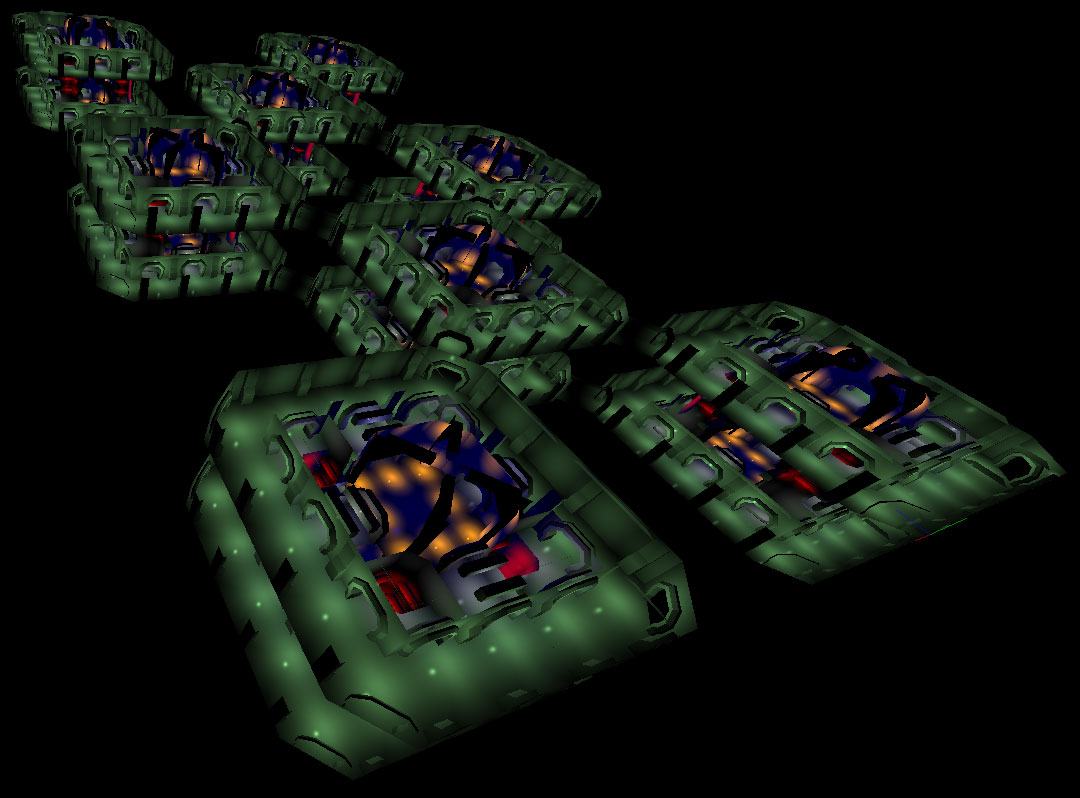
\includegraphics[width=\textwidth]{Images/Grid-Overview.jpg}
\captionfonts
\caption[The Grid Map Overview]{Overview of The Grid.}
\label{fig:grid-overview}

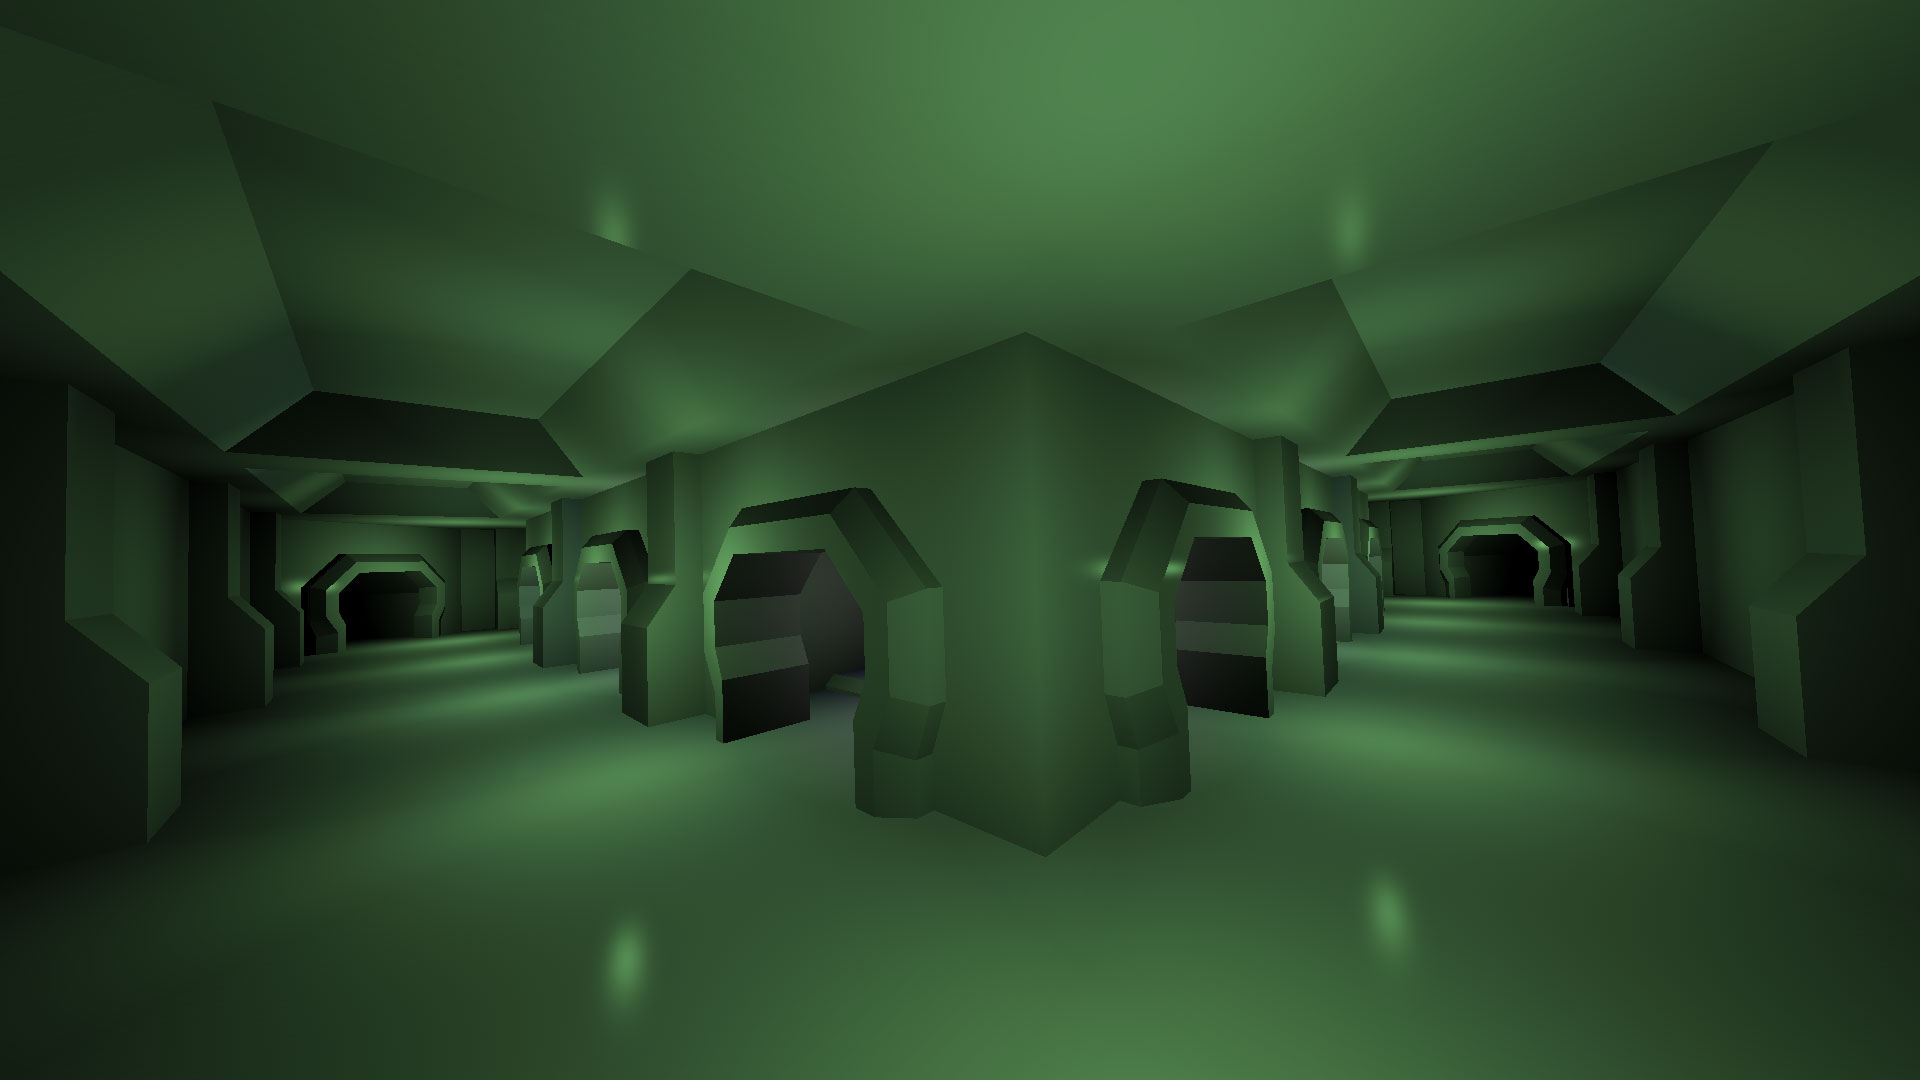
\includegraphics[width=\textwidth]{Images/GridHalls.jpg}
\captionfonts
\caption[Halls of the Grid]{A view of the outer hallways of The Grid.}
\label{fig:grid-halls}
\end{center}
\end{figure}

\begin{figure}
\begin{center}
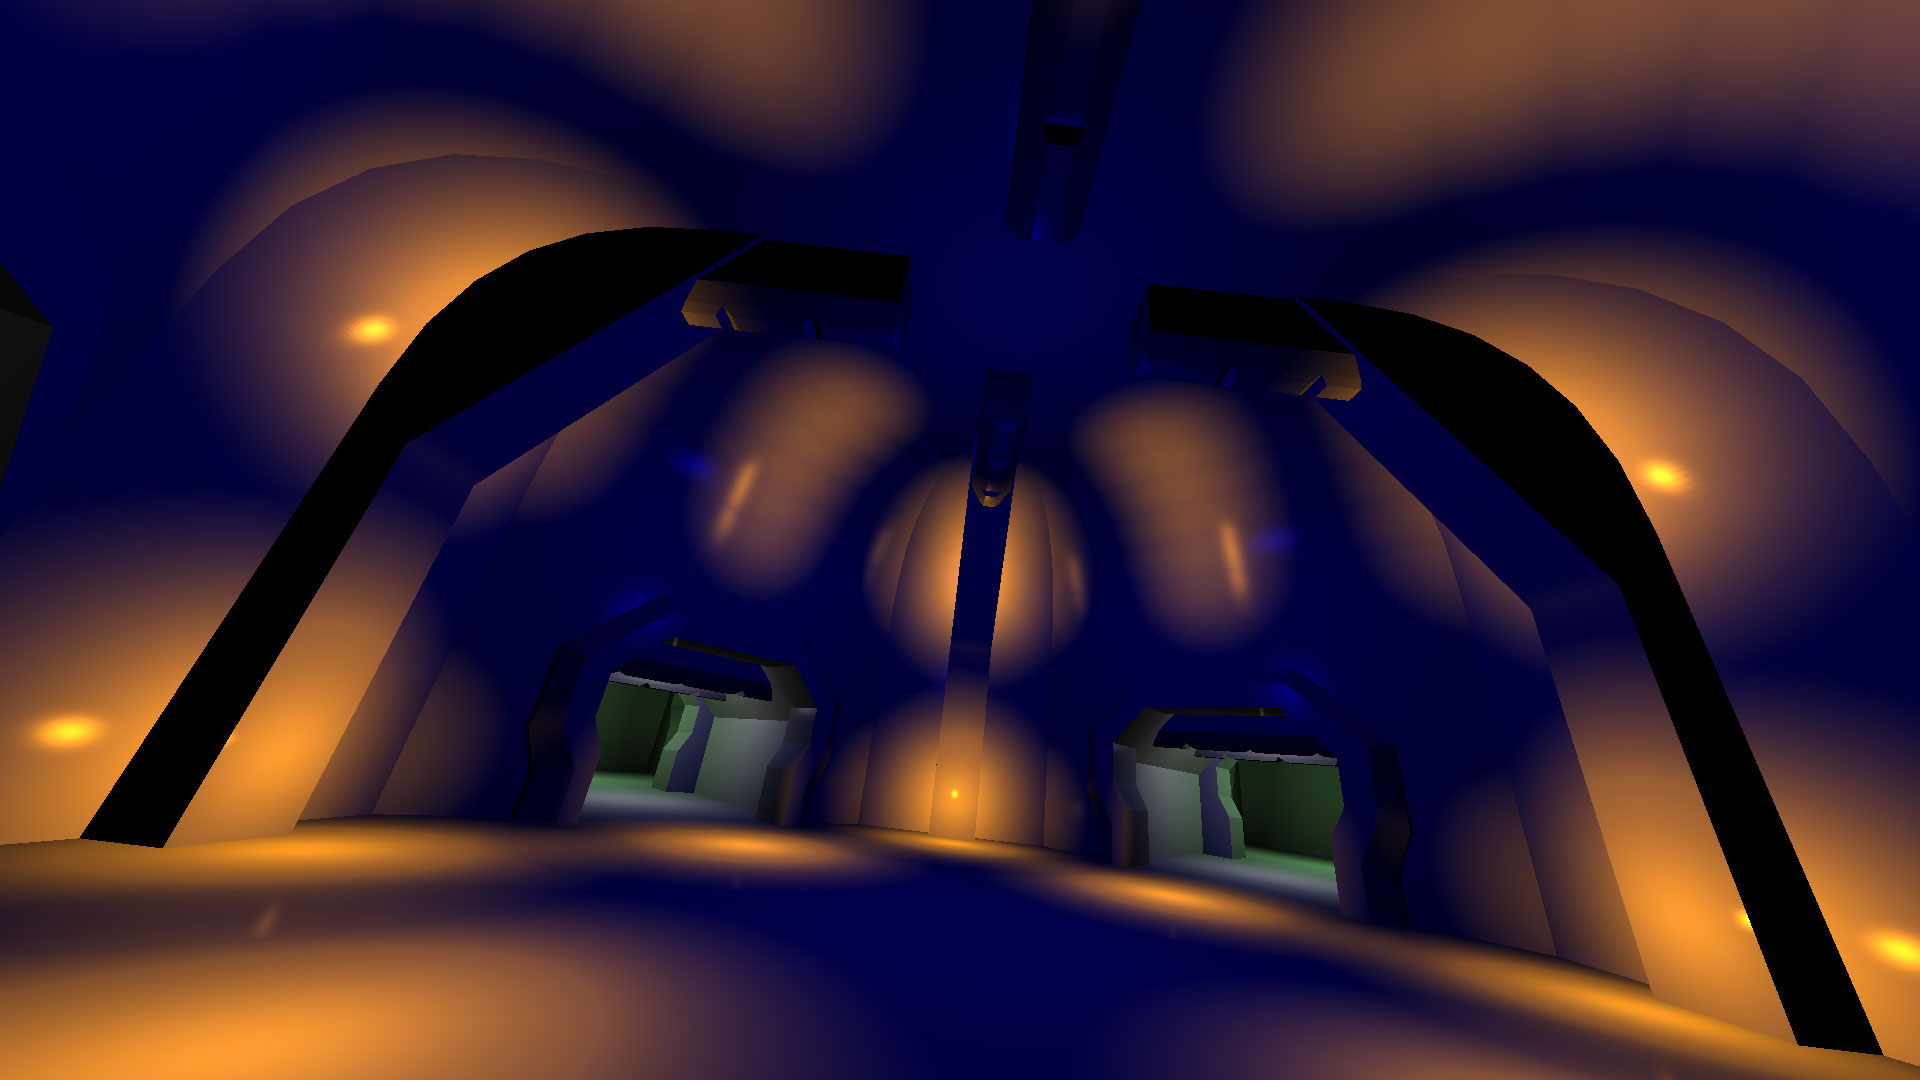
\includegraphics[width=\textwidth]{Images/GridInnerSanctum.jpg}
\captionfonts
\caption[Grid Inner Sanctum]{A view of the inner sanctum center area.}
\label{fig:grid-inner-sanctum}

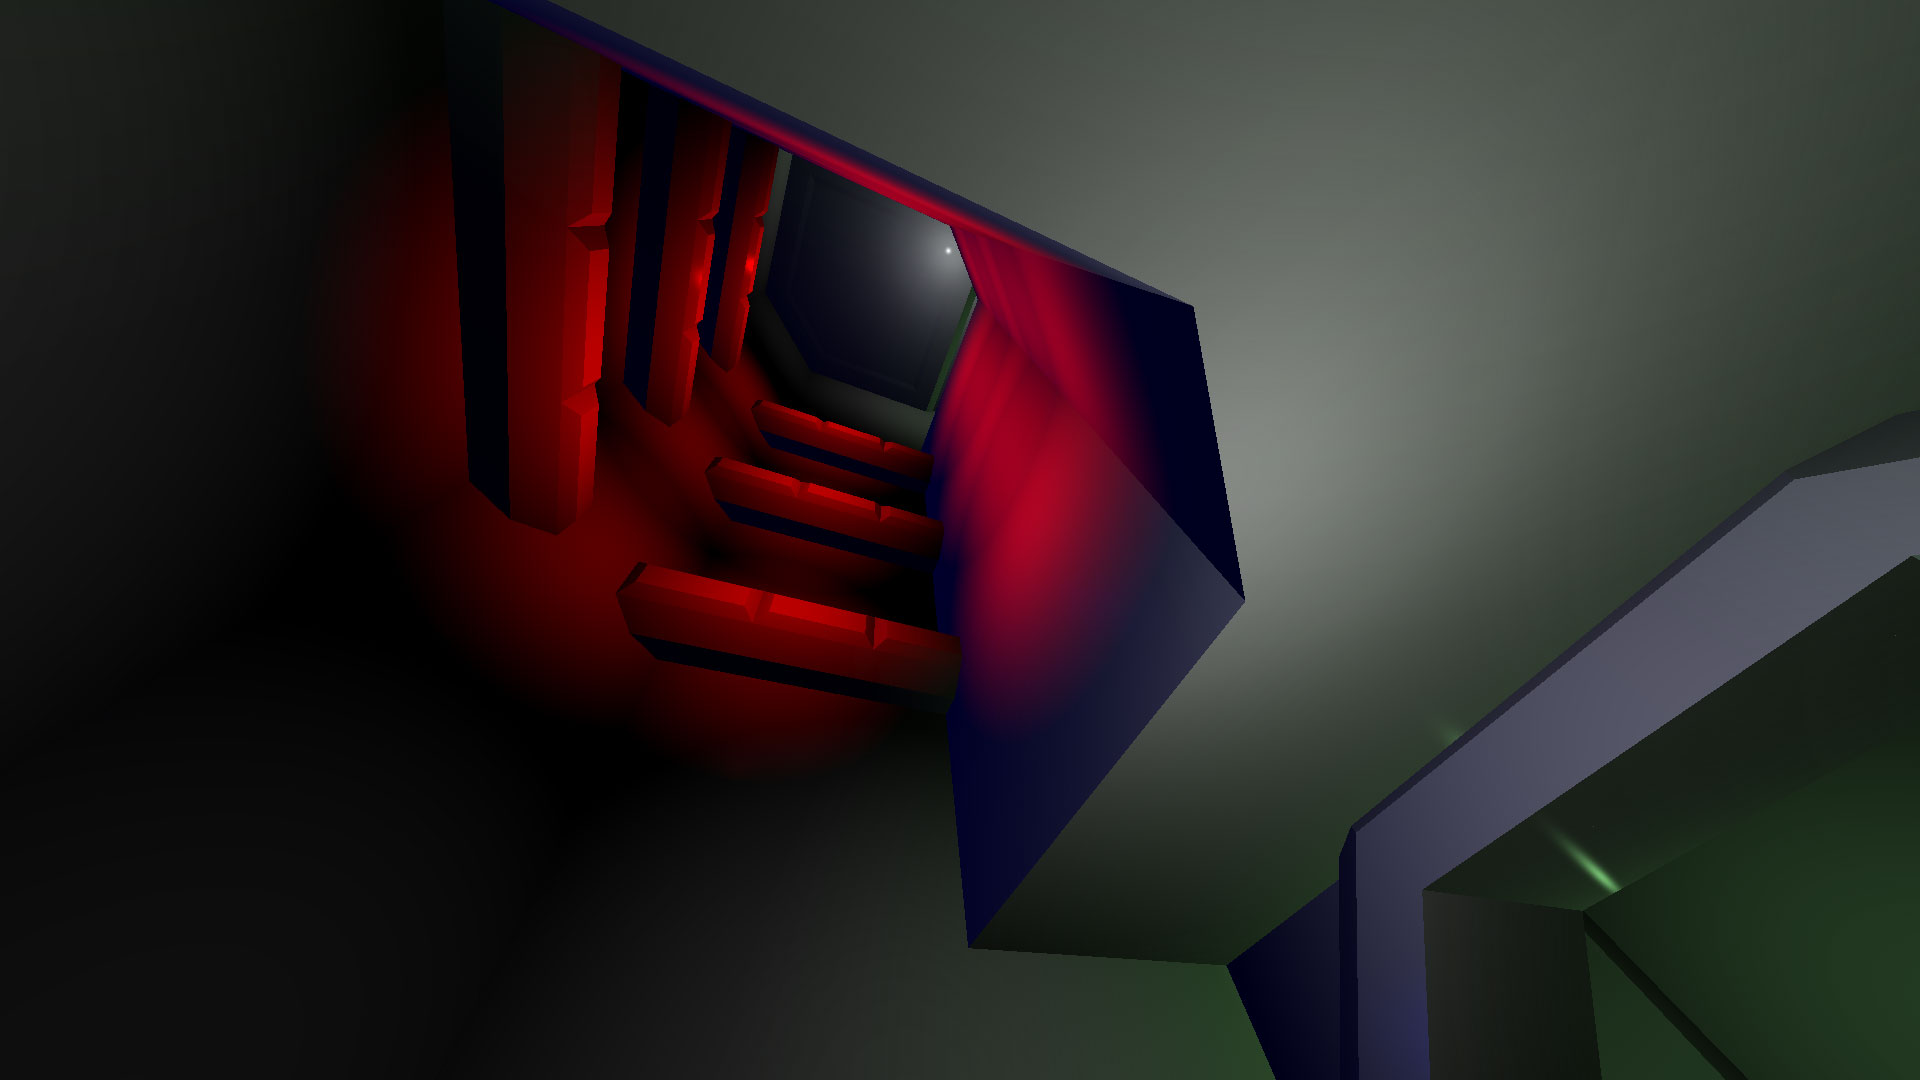
\includegraphics[width=\textwidth]{Images/GridShaft.jpg}
\captionfonts
\caption[Grid Shaft]{A view of the vertical shaft joining the two floors of The Grid.}
\label{fig:grid-shaft}

\end{center}
\end{figure}


\begin{figure}
\begin{center}
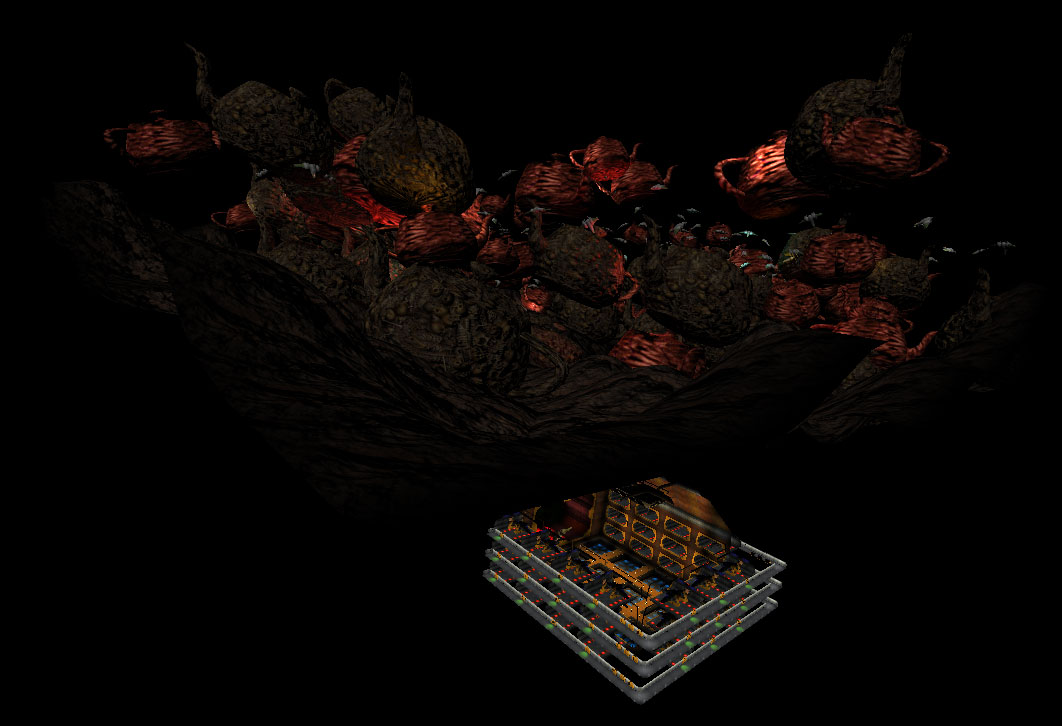
\includegraphics[width=\textwidth]{Images/GraveyardOverview.jpg}
\captionfonts
\caption[Teapot Graveyard Overview]{Overview of Teapot Graveyard.}
\label{fig:fraveyard-overview}

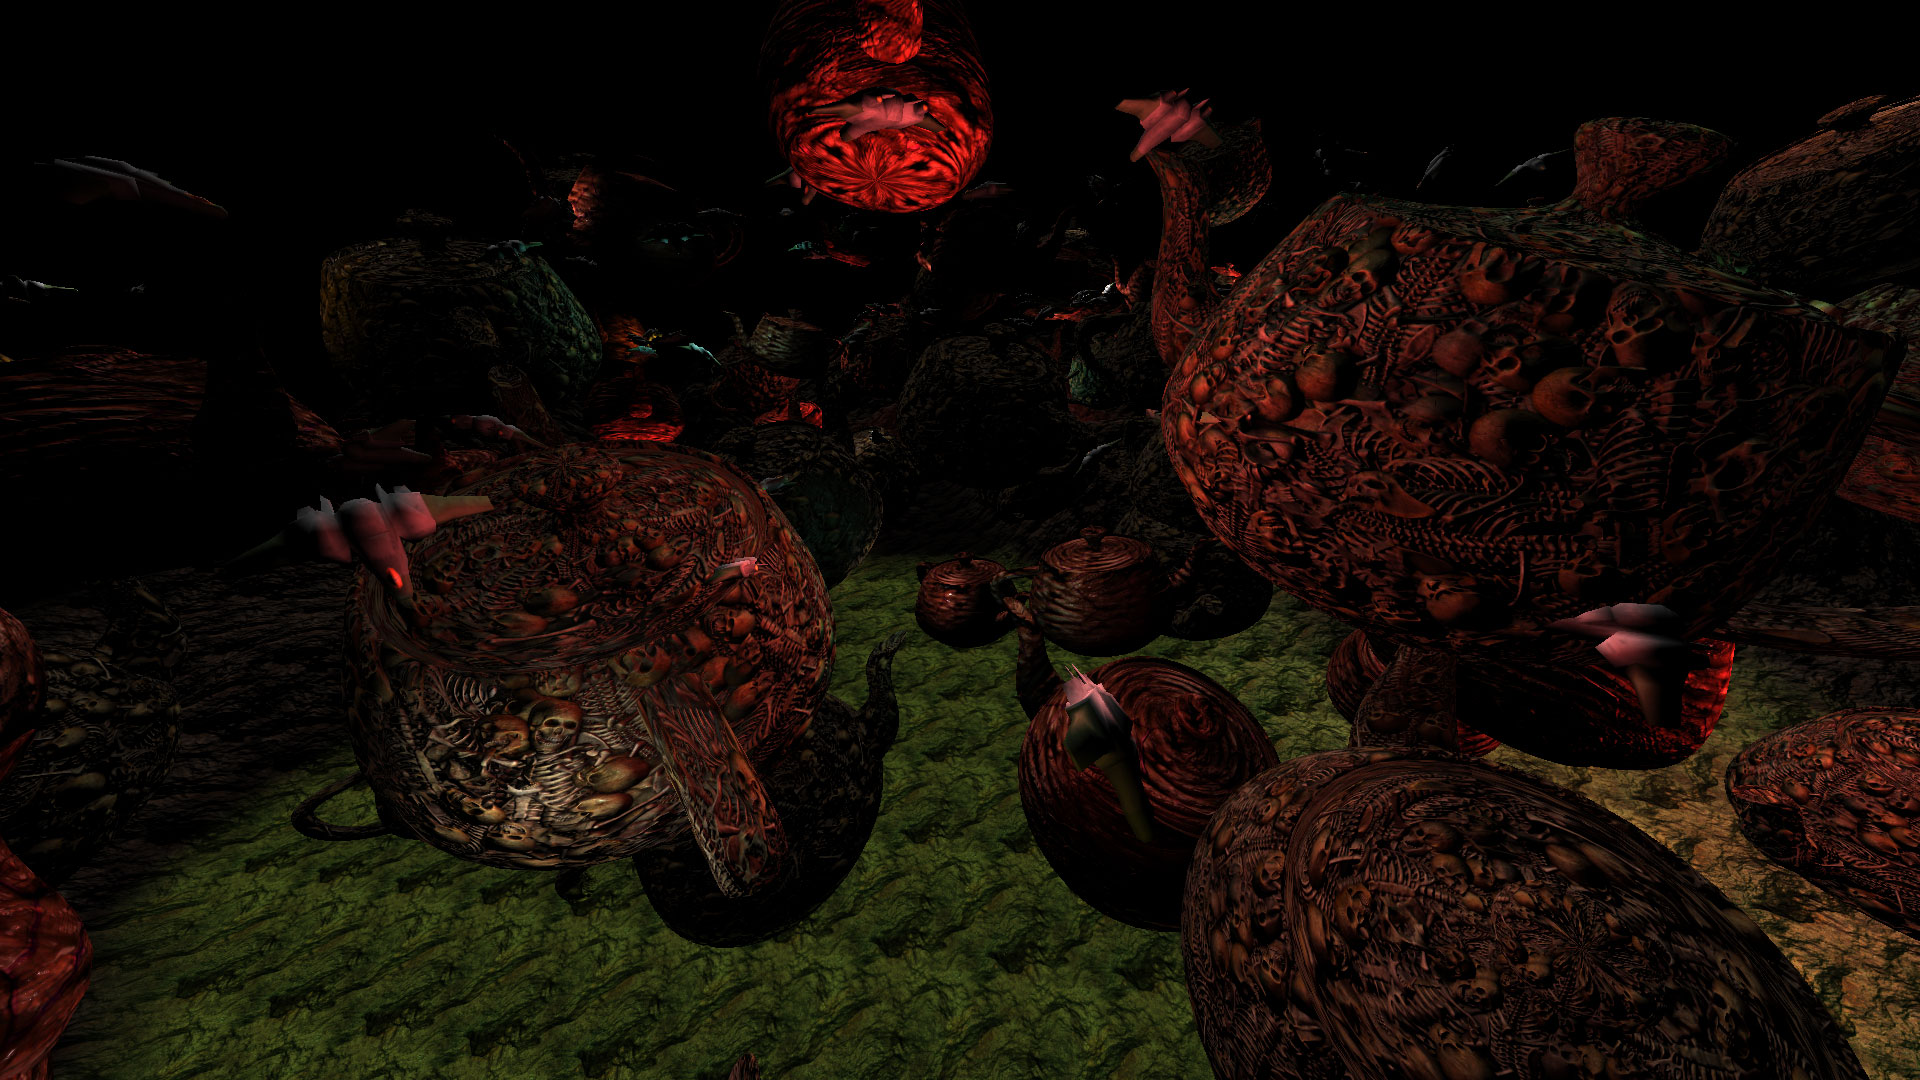
\includegraphics[width=\textwidth]{Images/TeapotGraveyard.jpg}
\captionfonts
\caption[Teapot Graveyard]{A view of the outdoor portion of the Teapot Graveyard map.}
\label{fig:teapot-graveyard}
\end{center}
\end{figure}

\begin{figure}
\begin{center}
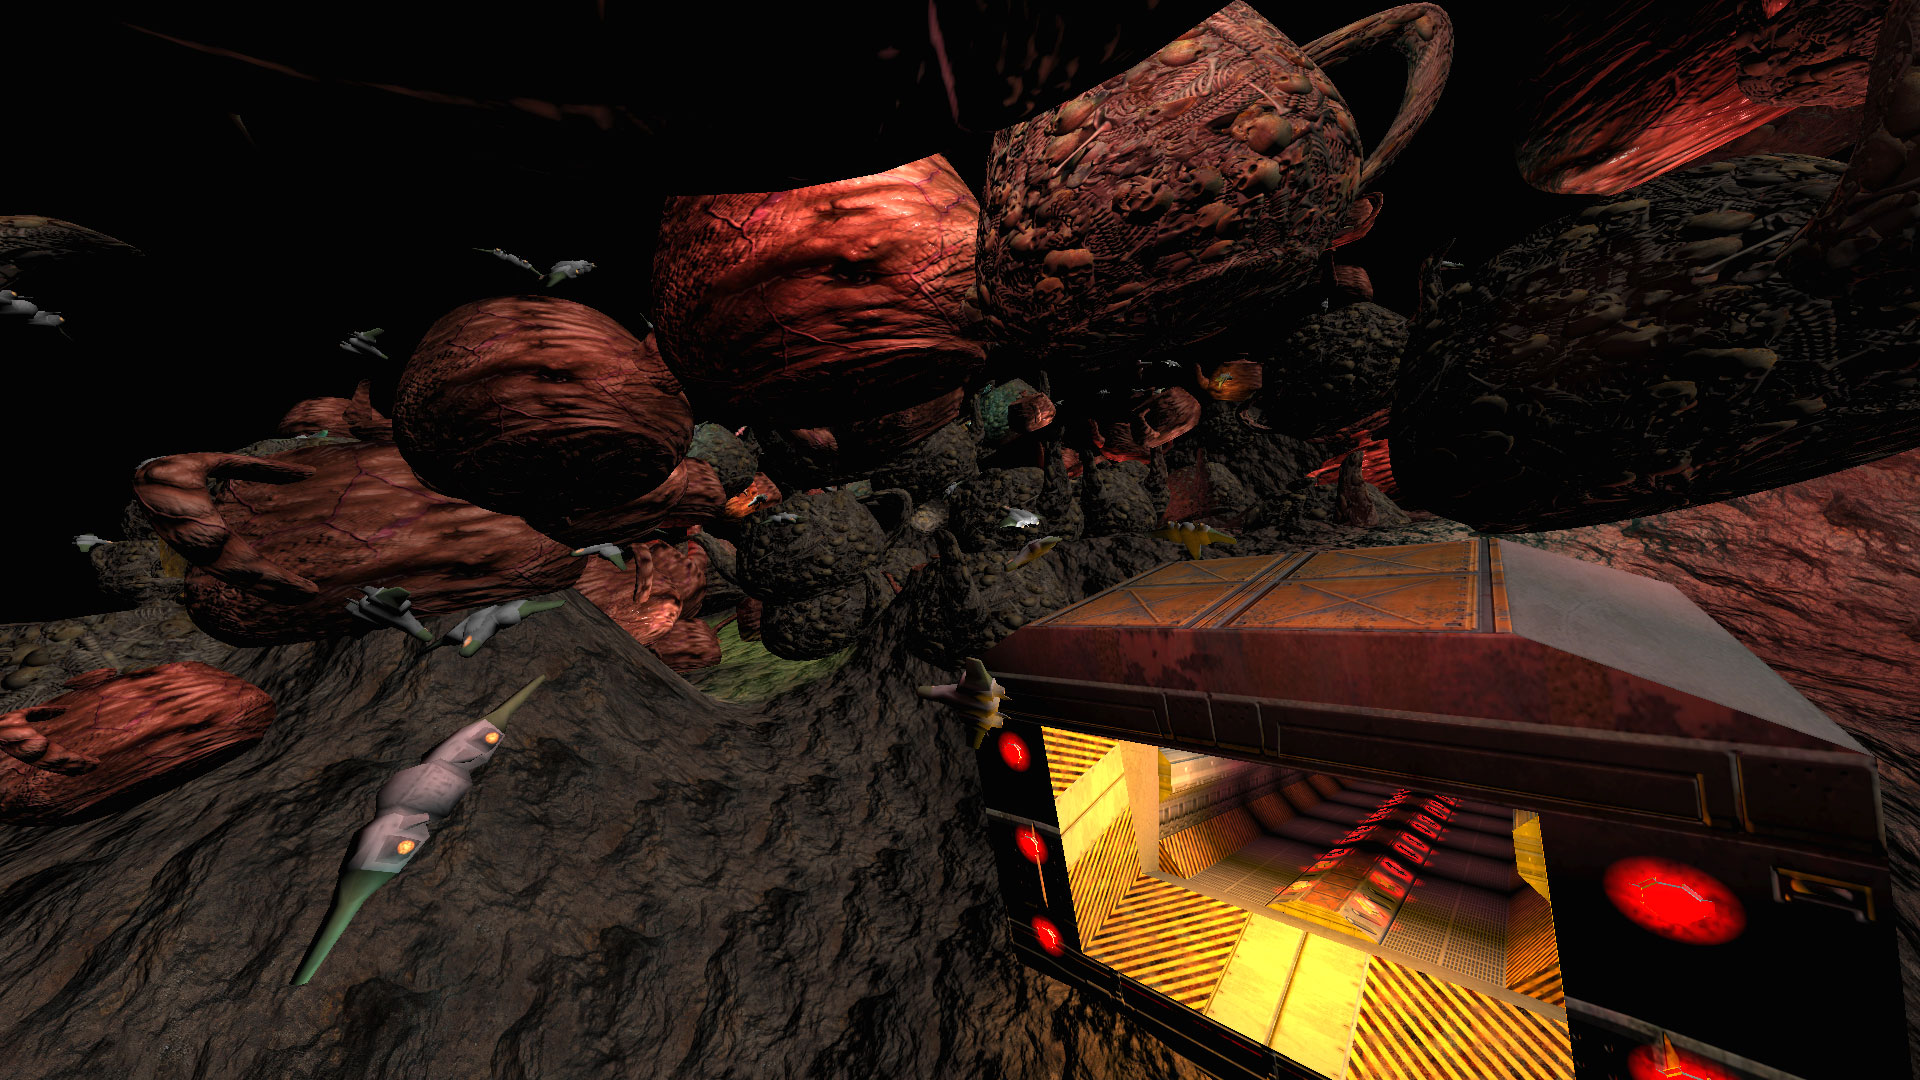
\includegraphics[width=\textwidth]{Images/HangarEntrance.jpg}
\captionfonts
\caption[Hangar Entrance]{Entrance into the Hangar area.}
\label{fig:hangar-entrance}

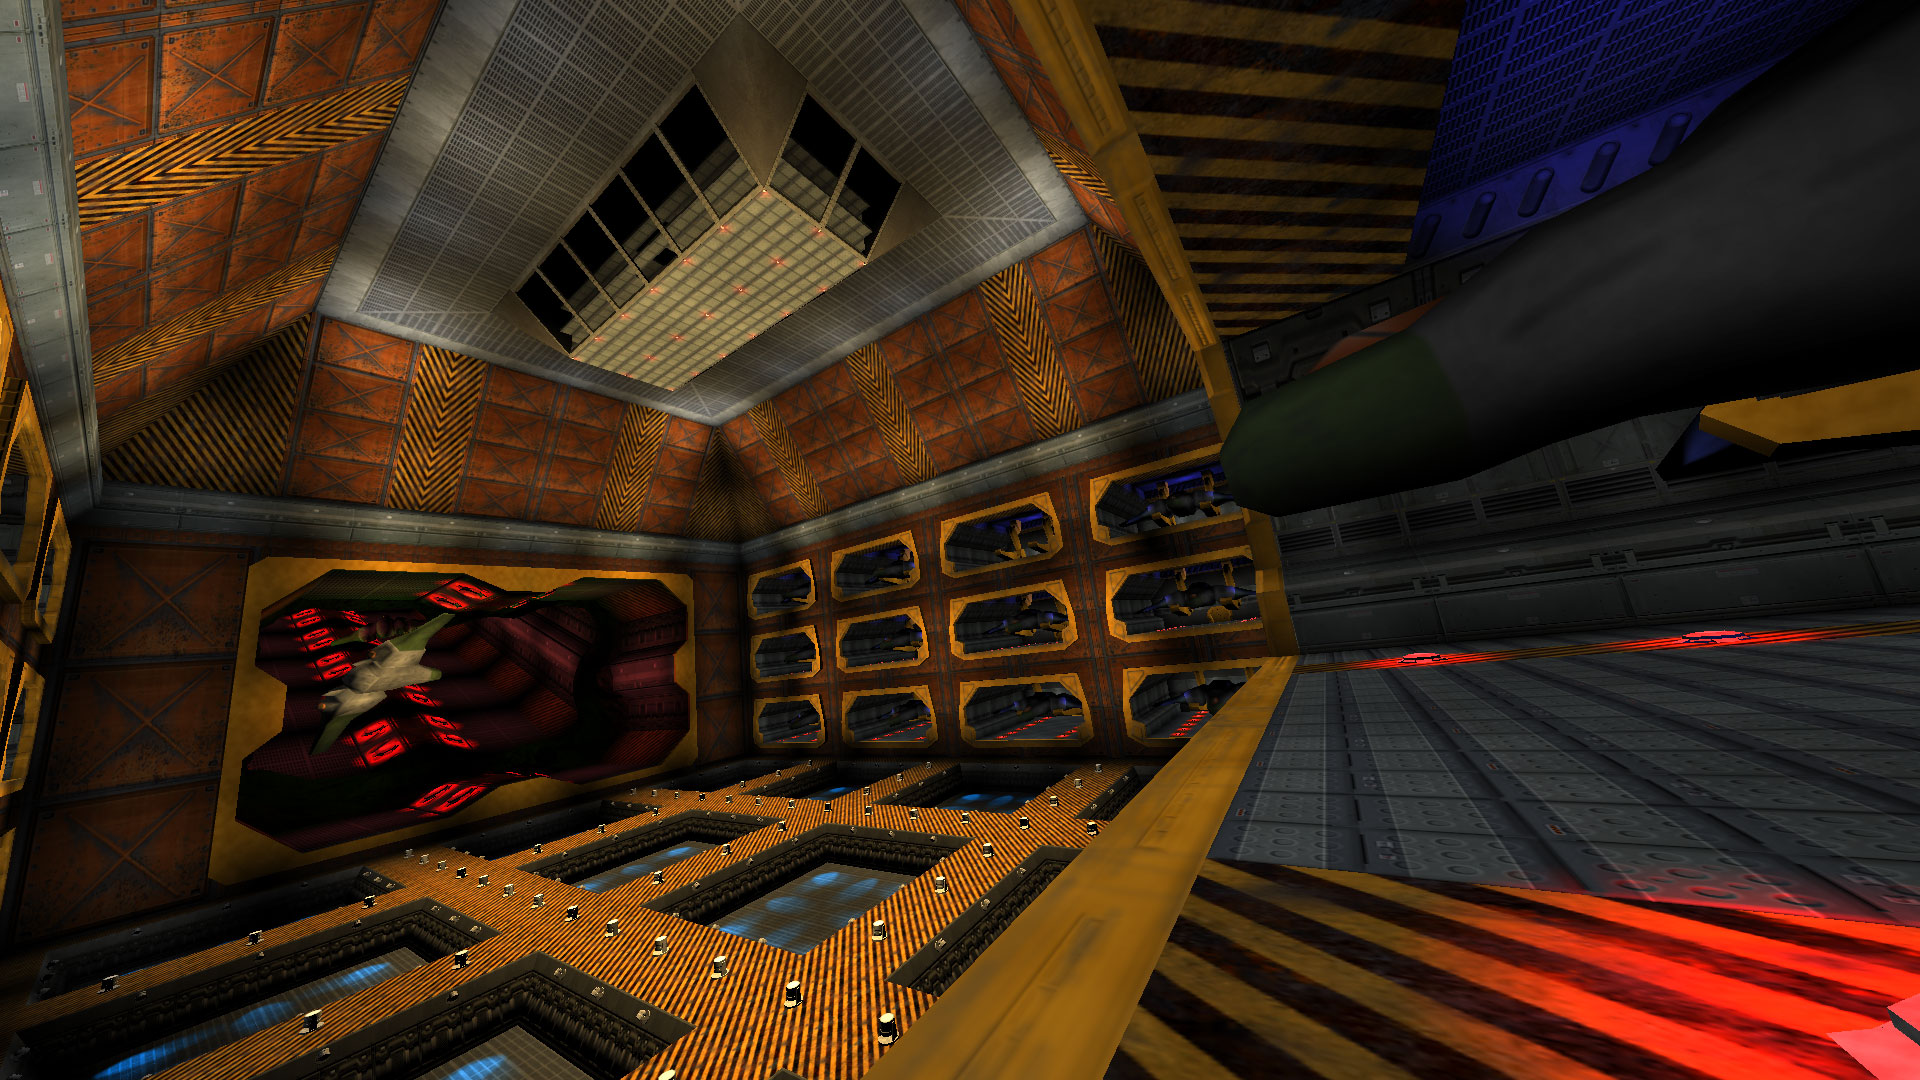
\includegraphics[width=\textwidth]{Images/Hangar.jpg}
\captionfonts
\caption[Hangar]{A view of the underground Hangar of the Teapot Graveyard.}
\label{fig:hangar}

\end{center}
\end{figure}

\begin{figure}
\begin{center}
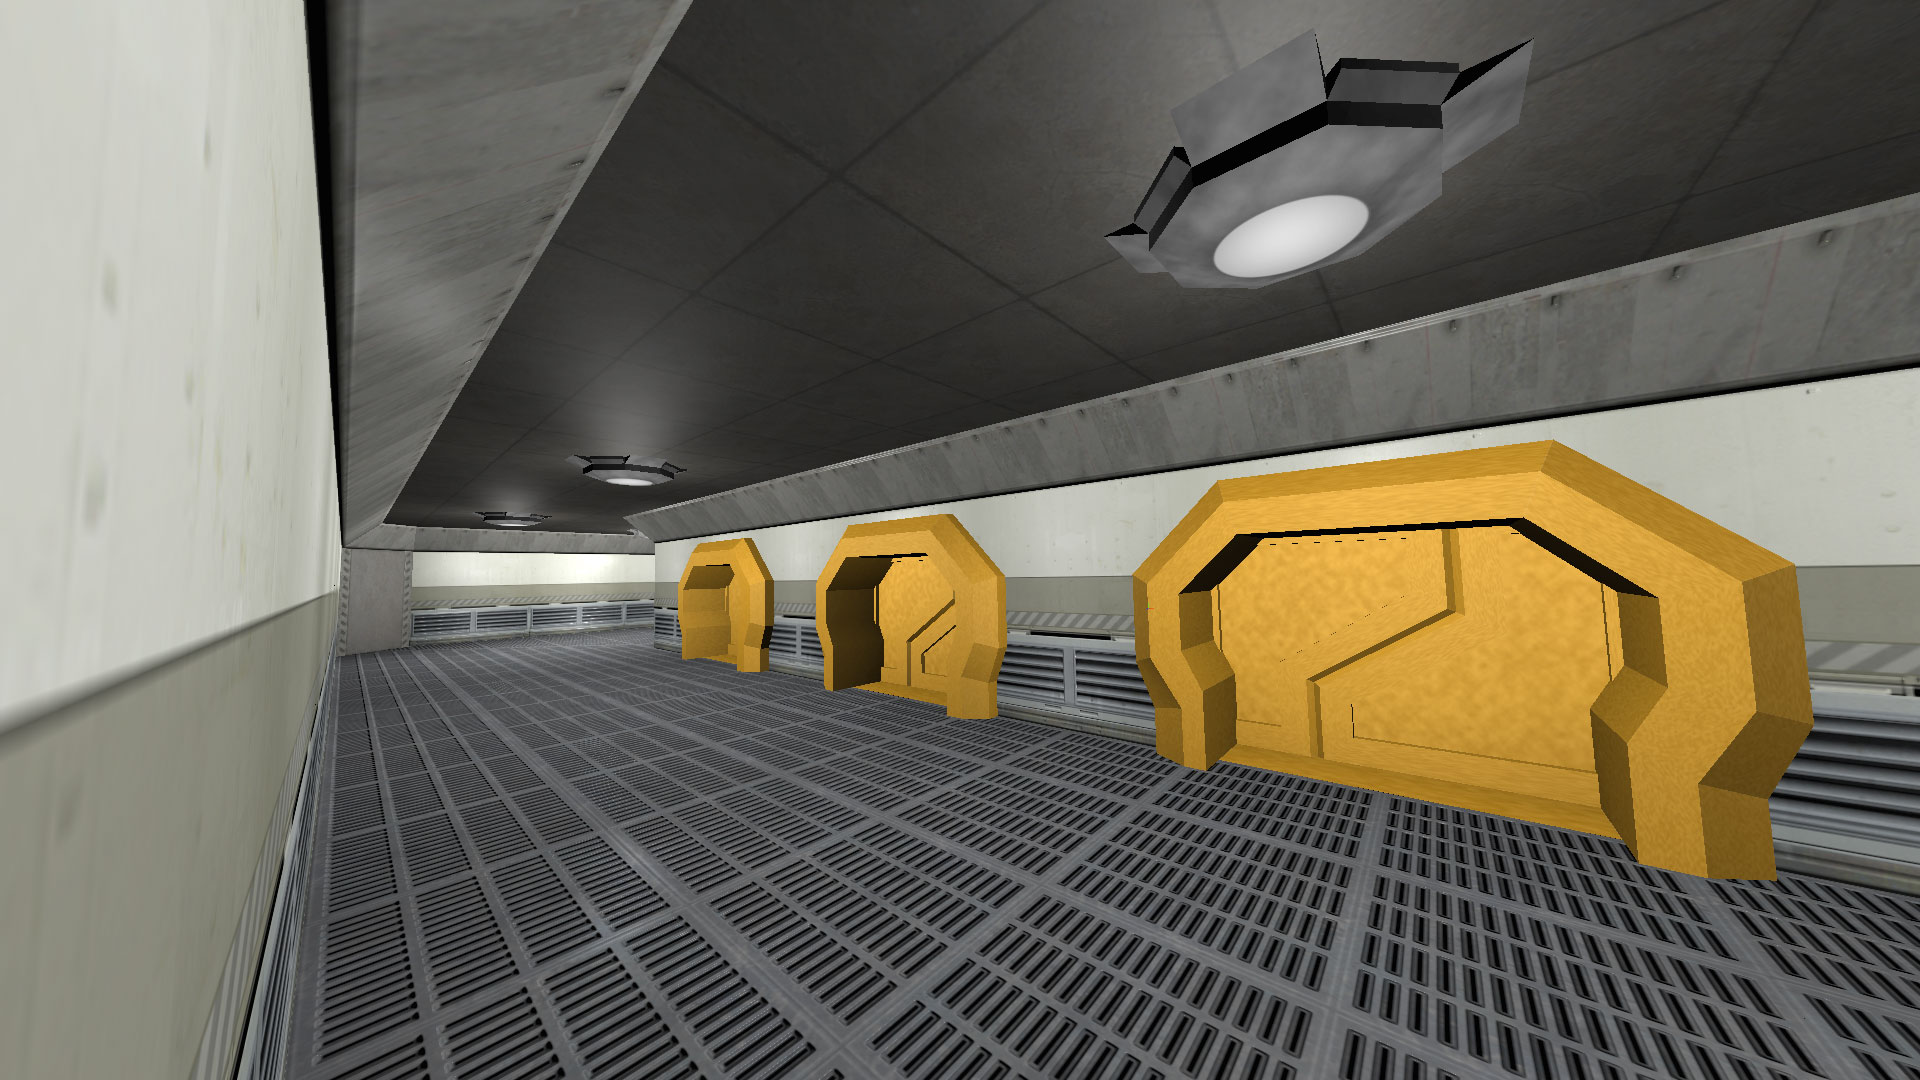
\includegraphics[width=\textwidth]{Images/HallCorner.jpg}
\captionfonts
\caption[Hall Corner]{Side hallways of the Hangar in Teapot Graveyard.}
\label{fig:hall-corner}

\end{center}
\end{figure}

\section {Metrics}
\label{metrics}

The most useful metrics for this engine are the framerate and the perceived popping artifacts.
The framerate is easily measurable and displayed with a graph that makes it easy to find causes of performance drops as the engine is running.
The measurement of popping artifacts directly would negatively affect performance.
A method for computing when an object or cell should be visible versus the amount of time it took for it to become visible would be difficult with the current implementation.
Knowing when an object should be visible is part of the algorithm in the first place, and the query cap causes a slight delay in visibility time of objects farther away.
As a result, measurement of popping artifacts is measured objectively.
The very core of this algorithm is to take advantage of the fact that people would not notice objects popping in too much, so this is the perfect way to measure the effectiveness of the algorithm.
(TODO, in the short amount of time I have, find a group of people to test my engine and report how much they noticed objects popping in.  So far I tested on myself only)
X people were asked to try running the engine with various settings and reported the degree of perceived noticeable pop in as either Not Noticeable, A Tiny Bit Noticeable, Sometimes Noticeable, and Very Noticeable.

%\begin{figure}
%\begin{center}
%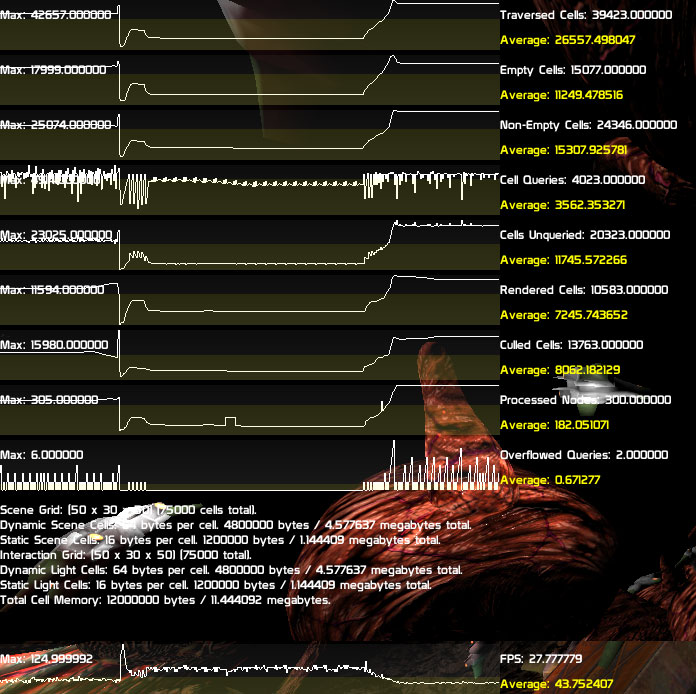
\includegraphics[width=\textwidth]{Images/PerfGraph.jpg}
%\captionfonts
%\caption[Performance Graph]{A graph showing performance statistics on the fly.}
%\label{fig:performance-graph}
%\end{center}
%\end{figure}

The variables are the grid dimensions, maximum queries per frame, validity duration of a visibility query, validity duration of an invisibility query, and the growth of duration for the two query results due to the number of frames in a row the query cap has been reached.

\section {Data}
\label{data}

\subsection {The Grid Map on GTX 480 Desktop PC}
\label{the-grid-gtx-480}

\begin{table}
\begin{center}
\begin{tabular}{|c|c|c|c|c|c|c|}
\hline 
&\multicolumn{2}{c|}{Visibility}&\multicolumn{2}{c|}{Invisibility}&&
\tabularnewline
Max Queries&Duration&Growth&Duration&Growth&FPS&Pop-in
\tabularnewline
\hline
1000 & 15& 4& 1& 1& 60& High
\tabularnewline
& 20& 6& 2& 1& 60& High
\tabularnewline
& 30& 8& 2& 2& 60& High
\tabularnewline \hline
2000 & 15& 4& 1& 1& 60& Medium
\tabularnewline
& 20& 6& 2& 1& 60& Medium
\tabularnewline
& 30& 8& 2& 2& 60& Medium
\tabularnewline \hline
3000 & 15& 4& 1& 1& 60& Low
\tabularnewline
& 20& 6& 2& 1& 60& Low
\tabularnewline
& 30& 8& 2& 2& 60& Low
\tabularnewline \hline 
4000 & 15& 4& 1& 1& 60& Unnoticeable
\tabularnewline 
& 20& 6& 2& 1& 60& Unnoticeable
\tabularnewline
& 30& 8& 2& 2& 60& Unnoticeable
\tabularnewline \hline 
\end{tabular}
\captionfonts
\caption[Performance for The Grid]{Cell dimensions: 5x12x5\\Number of Cells: 26x2x42}
\label{table:the-grid-performance-a}
\end{center}
\end{table}

\begin{table}
\begin{center}
\begin{tabular}{|c|c|c|c|c|c|c|}
\hline 
&\multicolumn{2}{c|}{Visibility}&\multicolumn{2}{c|}{Invisibility}&&
\tabularnewline
Max Queries&Duration&Growth&Duration&Growth&FPS&Pop-in
\tabularnewline
\hline
1000 & 15& 4& 1& 1& 60& High
\tabularnewline
& 20& 6& 2& 1& 60& High
\tabularnewline
& 30& 8& 2& 2& 60& High
\tabularnewline \hline
2000 & 15& 4& 1& 1& 60& Medium
\tabularnewline
& 20& 6& 2& 1& 60& Medium
\tabularnewline
& 30& 8& 2& 2& 60& Medium
\tabularnewline \hline
3000 & 15& 4& 1& 1& 60& Low
\tabularnewline
& 20& 6& 2& 1& 60& Low
\tabularnewline
& 30& 8& 2& 2& 60& Low
\tabularnewline \hline 
4000 & 15& 4& 1& 1& 60& Unnoticeable
\tabularnewline 
& 20& 6& 2& 1& 60& Unnoticeable
\tabularnewline
& 30& 8& 2& 2& 60& Unnoticeable
\tabularnewline \hline 
\end{tabular}
\captionfonts
\caption[Performance for The Grid]{The Grid map.\\Cell dimensions: 5x12x5\\Number of Cells: 26x2x42}
\label{table:the-grid-performance-b}
\end{center}
\end{table}

\begin{table}
\begin{center}
\begin{tabular}{|c|c|c|c|c|c|c|}
\hline 
&\multicolumn{2}{c|}{Visibility}&\multicolumn{2}{c|}{Invisibility}&&
\tabularnewline
Max Queries&Duration&Growth&Duration&Growth&FPS&Pop-in
\tabularnewline
\hline
1000 & 15& 4& 1& 1& 60& High
\tabularnewline
& 20& 6& 2& 1& 60& High
\tabularnewline
& 30& 8& 2& 2& 60& High
\tabularnewline \hline
2000 & 15& 4& 1& 1& 60& Medium
\tabularnewline
& 20& 6& 2& 1& 60& Medium
\tabularnewline
& 30& 8& 2& 2& 60& Medium
\tabularnewline \hline
3000 & 15& 4& 1& 1& 60& Low
\tabularnewline
& 20& 6& 2& 1& 60& Low
\tabularnewline
& 30& 8& 2& 2& 60& Low
\tabularnewline \hline 
4000 & 15& 4& 1& 1& 60& Unnoticeable
\tabularnewline 
& 20& 6& 2& 1& 60& Unnoticeable
\tabularnewline
& 30& 8& 2& 2& 60& Unnoticeable
\tabularnewline \hline 
\end{tabular}
\captionfonts
\caption[Performance for The Grid]{The Grid map.\\Cell dimensions: 5x12x5\\Number of Cells: 26x2x42}
\label{table:the-grid-performance-c}
\end{center}
\end{table}

\begin{table}
\begin{center}
\begin{tabular}{|c|c|c|c|c|c|c|}
\hline 
&\multicolumn{2}{c|}{Visibility}&\multicolumn{2}{c|}{Invisibility}&&
\tabularnewline
Max Queries&Duration&Growth&Duration&Growth&FPS&Pop-in
\tabularnewline
\hline
1000 & 15& 4& 1& 1& 60& High
\tabularnewline
& 20& 6& 2& 1& 60& High
\tabularnewline
& 30& 8& 2& 2& 60& High
\tabularnewline \hline
2000 & 15& 4& 1& 1& 60& Medium
\tabularnewline
& 20& 6& 2& 1& 60& Medium
\tabularnewline
& 30& 8& 2& 2& 60& Medium
\tabularnewline \hline
3000 & 15& 4& 1& 1& 60& Low
\tabularnewline
& 20& 6& 2& 1& 60& Low
\tabularnewline
& 30& 8& 2& 2& 60& Low
\tabularnewline \hline 
4000 & 15& 4& 1& 1& 60& Unnoticeable
\tabularnewline 
& 20& 6& 2& 1& 60& Unnoticeable
\tabularnewline
& 30& 8& 2& 2& 60& Unnoticeable
\tabularnewline \hline 
\end{tabular}
\captionfonts
\caption[Performance for Teapot Graveyard]{Teapot Graveyard map.\\Cell dimensions: 5x12x5\\Number of Cells: 26x2x42}
\label{table:teapot-performance-a}
\end{center}
\end{table}

\begin{table}
\begin{center}
\begin{tabular}{|c|c|c|c|c|c|c|}
\hline 
&\multicolumn{2}{c|}{Visibility}&\multicolumn{2}{c|}{Invisibility}&&
\tabularnewline
Max Queries&Duration&Growth&Duration&Growth&FPS&Pop-in
\tabularnewline
\hline
1000 & 15& 4& 1& 1& 60& High
\tabularnewline
& 20& 6& 2& 1& 60& High
\tabularnewline
& 30& 8& 2& 2& 60& High
\tabularnewline \hline
2000 & 15& 4& 1& 1& 60& Medium
\tabularnewline
& 20& 6& 2& 1& 60& Medium
\tabularnewline
& 30& 8& 2& 2& 60& Medium
\tabularnewline \hline
3000 & 15& 4& 1& 1& 60& Low
\tabularnewline
& 20& 6& 2& 1& 60& Low
\tabularnewline
& 30& 8& 2& 2& 60& Low
\tabularnewline \hline 
4000 & 15& 4& 1& 1& 60& Unnoticeable
\tabularnewline 
& 20& 6& 2& 1& 60& Unnoticeable
\tabularnewline
& 30& 8& 2& 2& 60& Unnoticeable
\tabularnewline \hline 
\end{tabular}
\captionfonts
\caption[Performance for Teapot Graveyard]{Teapot Graveyard map.\\Cell dimensions: 5x12x5\\Number of Cells: 26x2x42}
\label{table:teapot-performance-b}
\end{center}
\end{table}

\begin{table}
\begin{center}
\begin{tabular}{|c|c|c|c|c|c|c|}
\hline 
&\multicolumn{2}{c|}{Visibility}&\multicolumn{2}{c|}{Invisibility}&&
\tabularnewline
Max Queries&Duration&Growth&Duration&Growth&FPS&Pop-in
\tabularnewline
\hline
1000 & 15& 4& 1& 1& 60& High
\tabularnewline
& 20& 6& 2& 1& 60& High
\tabularnewline
& 30& 8& 2& 2& 60& High
\tabularnewline \hline
2000 & 15& 4& 1& 1& 60& Medium
\tabularnewline
& 20& 6& 2& 1& 60& Medium
\tabularnewline
& 30& 8& 2& 2& 60& Medium
\tabularnewline \hline
3000 & 15& 4& 1& 1& 60& Low
\tabularnewline
& 20& 6& 2& 1& 60& Low
\tabularnewline
& 30& 8& 2& 2& 60& Low
\tabularnewline \hline 
4000 & 15& 4& 1& 1& 60& Unnoticeable
\tabularnewline 
& 20& 6& 2& 1& 60& Unnoticeable
\tabularnewline
& 30& 8& 2& 2& 60& Unnoticeable
\tabularnewline \hline 
\end{tabular}
\captionfonts
\caption[Performance for Teapot Graveyard]{Teapot Graveyard map.\\Cell dimensions: 5x12x5\\Number of Cells: 26x2x42}
\label{table:teapot-performance-c}
\end{center}
\end{table}

\section{Conclusions}
\label{conclusions}
These results show that a maximum of about 3000 to 4000 queries gives the best balance between performance and perceived object pop in.
The large outdoor Teapot Graveyard map benefits from a denser grid when exploring the underground hangar area.
This section contains tight indoor corridors, and having a denser grid allows the engine to avoid rendering more objects behind walls.
The outdoor portion doesn't show benefit from a denser grid, so maps that are exclusively outdoors should stick to using sparser grids.

The indoor map, The Grid, doesn't hit the query maximum as much.
Even with a more dense grid than Teapot Graveyard, there are less grid cells to rasterize since the map dimensions are smaller.
This map tends to keep up a high framerate at all times, showing how well this algorithm performs in the kinds of environments that are usually rendered with portal culling and other static indoor environment techniques.

These tests have shown that the visibility culling algorithm presented in this paper is effective for both indoor and outdoor environments.
Although hardware occlusion queries can cause CPU stalls, using them wisely can be very beneficial.
By taking advantage of spatial and temporal coherence, we were able to push performance out of an often overlooked feature of the graphics pipeline.

\chapter{Future Work}
\label{future-work}
As mentioned earlier, the current deferred shading renderer is limited to rendering only solid objects.
Static multimaterial triangle meshes are the only type of object renderable, which was enough to create the detailed scenes used for testing the algorithm.
Transparent objects would require a forward shading renderer.
The approximate front to back frustum traversal algorithm would work great for sorting alpha blended objects in the correct order since only occlusion order is needed, not true depth order.
Skeletal animations, particle systems, shadows, and various post processing effects would add even more stress to the engine, giving more opportunity to find ways to optimize the algorithm.

Cascaded shadow maps are often used for large outdoor environments to cast shadows from sunlight or other global outdoor sources.\cite{ms-cascaded-shadow}
The paper mentioned earlier a method for supporting multiple viewports for split screen multiplayer.
A viewport can be created for the point of view of the outdoor global light source since a large portion of the scene needs to be rendered to the shadow map.
For smaller light volumes, it's best to avoid using the hardware occlusion queries and to just render objects that are within the view frustum from the light's point of view.
The bookkeeping required for each viewport that uses this algorithm would be impractical for that many lights.

The graphics engine was originally a fully featured multi threaded game engine.
It was driven by a combination of Nvidia PhysX 3.0 and Intel Thread Building Blocks.
Those features were stripped out for the current implementation in favor of a single threaded graphics only engine in order to avoid being distracted by other features.
Seeing a fully functional world with moving objects being driven by this graphics engine would be a great stress test.
Being in an action packed world would likely reduce how noticeable popping is.
The CPU stall from gathering query results from last frame mentioned earlier would be less impactful since the engine has more work to do.
The query results would likely be ready by the time the engine is done updating the rest of the game.
There may also be room for parallelizing some portions of this algorithm, such as the sorting of alpha blended objects mentioned earlier.

% ------------- End main chapters ----------------------

\clearpage
\bibliography{bibliography}
\bibliographystyle{plain}
%\addcontentsline{toc}{chapter}{Bibliography}

\end{document}